\documentclass[a4paper,11pt]{article}

\usepackage{amsfonts}
\usepackage{amsmath}
\usepackage{amssymb}
\usepackage{graphicx}
\usepackage[utf8]{inputenc}
\usepackage[polish]{babel}
\usepackage[T1]{fontenc}
\usepackage[margin=.9in, footskip=.25in, bottom=0.5in]{geometry}

\setlength{\abovecaptionskip}{-5pt plus 5pt minus 0pt}  

%----------------------
\def\\{\hfill\break}
%----------------------

\title{Projekt Egzaminacyjny}
\author{Marcin Wojciechowski, Szymon Wierzejski}
\date{Listopad 2023 -- Styczeń 2024}

\begin{document}

\maketitle
\newpage

\tableofcontents
\newpage

\vspace*{4cm}
\section{Wstęp}
\textbf{Warner Music Group (WMG.US)} to jedna z czterech wielkich wytwórni płytowych branży muzycznej. Według raportu Nielson SoundScan z 2012r. miała ona udział 19,15\% w światowym rynku muzycznym. Do najważniejszych wytwórni należących do WMG należą: Atlantic Records - wytwórnia muzyki rhytm and blues, Elektra Records - wytwórnia muzyki folkowej, Bad Boy Records - hip-hop i Warner Records. Na giełdzie spółka debiutowała w 2005 roku na New York Stock Exchange (Nyse). Stan ten utrzymał się do 2011 roku, kiedy została ona sprywatyzowana i sprzedana Access Industries. Drugi debiut nastąpił w 2020 roku na Nasdaq Stock Market i od tego czasu spółka jest tam nieprzerwanie notowana do dziś.

\smallskip

\textbf{11 Bit Studios (11B)} to polskie przedsiębiorstwo z siedzibą w Warszawie zajmujące się produkcją i wydawaniem gier komputerowych. Założone w 2009 roku i już w 2010 debiutowało na alternatywnym rynku Giełdy Papierów Wartościowych, na rynku NewConnect. Pod koniec roku 2015 spółki firmy były już dostępne na głównym parkiecie Giełdy Papierów Wartościowych. Studio 11 Bit zasłynęło z gier Anomaly: Warzone Earth (2011), This War of Mine (2014) i Frostpunk (2018). Szczególnie wyróżnia się fakt, że produkt tego studia jest pierwszą grą cyfrową, w historii polskiej edukacji, wpisaną w rejestr lektur szkolnych i jest nią "This War of Mine".

\newpage
\section {Analiza cen spółek WMG.US i 11B}
Projekt egazminacyjny z modelowania matematycznego, chcielibyśmy zacząć od analizy cen spółek WMG.US i 11B. Analiza obejmować będzie kolejno: statystiki opisowe, wykresy diagnostyczne, a także testowanie hipotezy o równości rozkładów

\smallskip

\subsection{Spółka WMG.US}
Rozpoczniemy od analizy cen akcji spółki WMG.US. Pierwszym krokiem będzie przyjrzenie się statystykom opisowym.
\subsubsection{Wykres cen zamknięcia akcji i histogram}
Poniżej znajdują się wykres kursów zamknięcia pokazujący zmiany w czasie oraz histogram gęstości dla cen spółki WMG.US

\begin{figure}[h]
\centering
\begin{minipage}[b]{0.40\textwidth}
\centering
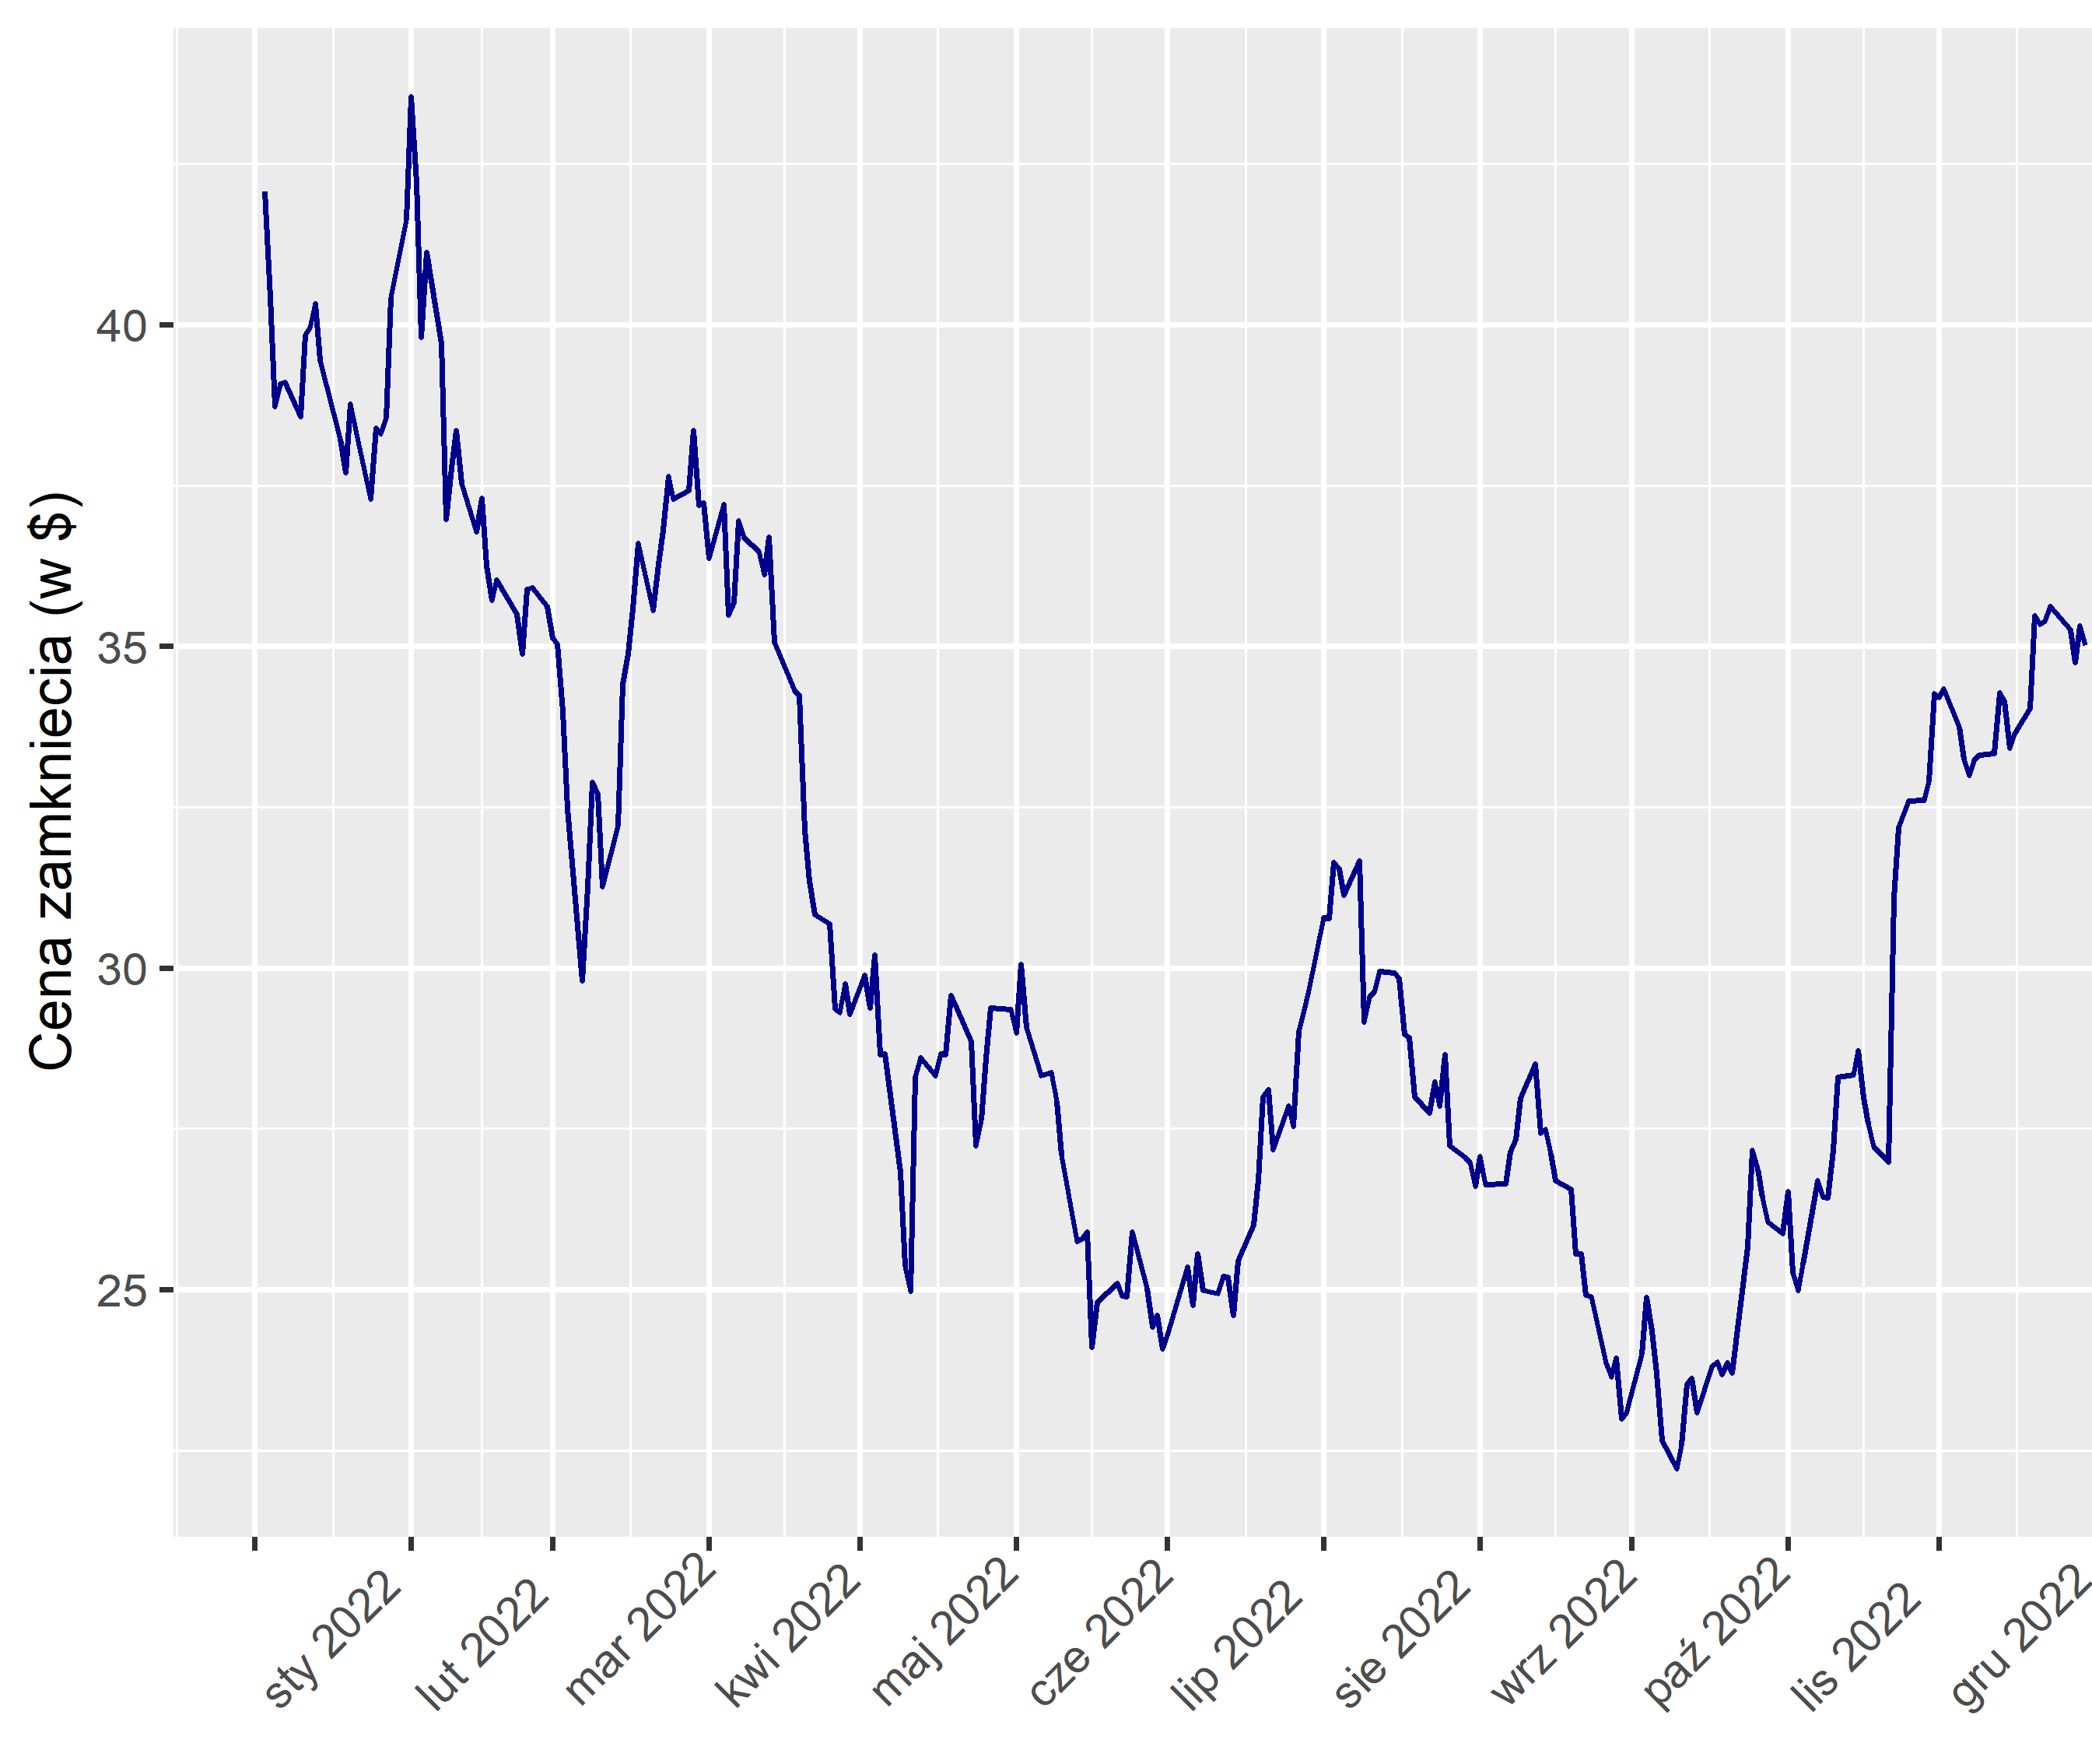
\includegraphics[width=\textwidth, height=5.2cm, width = 7cm]{img/Wykres_cen_akcji_WMG.png}
\caption{Wykres cen zamknięcia akcji pokazujący zmiany w czasie - WMG.US}
\label{fig:r3}
\end{minipage}
\hfill
\begin{minipage}[b]{0.40\textwidth}
\centering
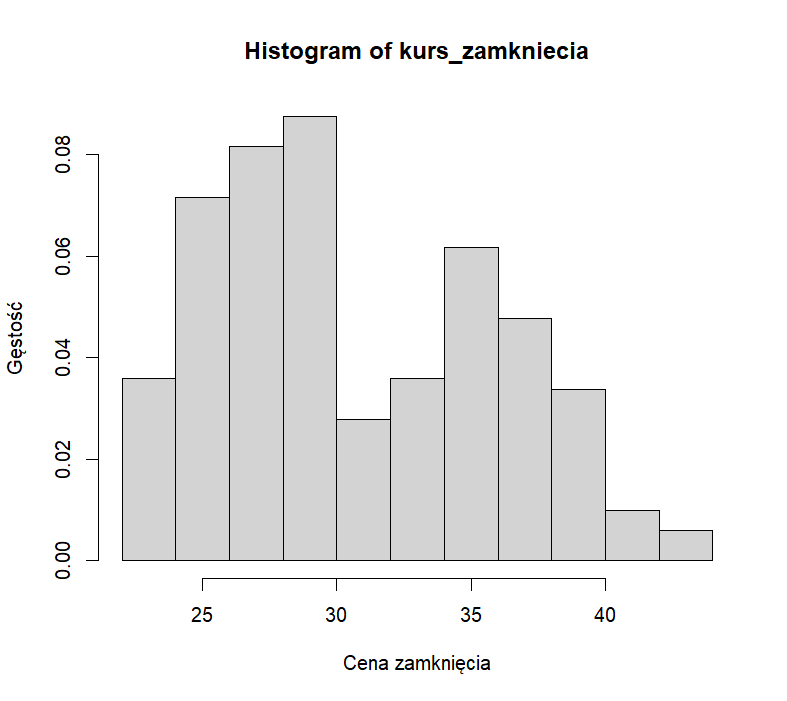
\includegraphics[width=\textwidth, height=5.25cm, width = 7cm]{img/Histogram_kursu_zamkniecia_WMG.png}
\caption{Histogram cen zamknięcia - WMG.US}
\label{fig:r4}
\end{minipage}
\end{figure}

\subsubsection{Statystyki opisowe}

Obliczone statystki opisowe:
\vspace*{0.2cm}

\centerline{\begin{tabular}{|c|c|c|c|c|}
\hline
 & $\bar{x}$ & odch. st. & skośność & kurtoza \\
\hline
Akcja & 30.701 & 5.104 & 0.386 & -0.991 \\
\hline
\end{tabular}}

\vspace*{0.5cm}

Interpretacja statystyk:

- Średnia z przedstawionych danych wynosi 30.7

- Stosunkowo duża wartość odchylenia standardowego świadczy o dużym rozproszeniu danych, można to zauważyć na przedstawionym powyżej histogramie

- Dodatnia skośność wskazuje na prawostronną asymetrię rozkładu, a co za tym idzie, wydłużony prawy ogon, w kierunku wyższych cen zamknięcia. Więcej danych jest skupionych wokół niższych wartości.

- Ujemna kurtoza wskazuje, że w danych istnieje mniej dodatnich wartości odstających niż w przypadku rozkładu normalnego, co oznacza, że wartości występujące w ogonach są mniej prawdopodobne w porównaniu do ich prawdopodobieństwa w rozkładzie normalnym

\subsubsection{Estymacja parametrów rozkładów}

W kontekście analizy danych, dokonana została estymacja parametrów trzech różnych rozkładów: rozkładu normalnego, log-normalnego oraz gamma. Poniższa tabela przedstawia uzyskane wyniki:
\vspace*{0.3cm}

\centerline{\begin{tabular}{|c|cc|cc|cc|}
\hline
& \multicolumn{2}{c|}{\textbf{r. normalny}} 
& \multicolumn{2}{c|}{\textbf{r. log-normalny}}                        
& \multicolumn{2}{c|}{\textbf{r. gamma}} \\ \hline
parametr & mean & sd & meanlog & sdlog & shape & rate \\ \hline
estymacja & 30.7 & 5.09 & 3.41 & 0.16 & 37.12 & 1.21 \\ \hline
std. bląd & 0.32 & 0.23 & 0.01 & 0.01 & 3.3 & 0.11 \\ \hline
\end{tabular}}

\vspace*{0.5cm}

Dla rozkładu normalnego "mean" oznacza przesunięcie rozkładu bez zmiany jego kształtu, natomiast "sd" oznacza jak bardzo "położony" jest wykres, w tym przypadku jest ono znacznie większe, od domyślnego rozkładu normalnego.

Dla rozkładu log-normalnego "meanlog" przyjmuje to samo znaczenie, co dla rozkładu normalnego "mean", natomiast "sdlog" różni się tym, że jest to odchylenie standardowe od normalnego logarytmu, a nie od samego X.

Dla rozkładu gamma "shape" jest parametrem kształtu, czyli wpływa on zarówno na przesunięcie, wielkość, ale także kształt rozkładu, natomiast "rate" jest odwrotnością parametru skali, jednego z dwóch parametrów rozkładu gamma.

Wyniki estymacji rozkładów pokazują, że rozkład log-normalny ma niskie wartości parametrów i najniższą wartość błędu standardowego w porównaniu z innymi analizowanymi rozkładami. Natomiast wyestymowane parametry i błąd standardowy rozkładu gamma przyjmują bardzo wysokie wartości.

\subsubsection{Wykresy diagnostyczne. Analiza wartości statystyk.}
Poniżej przedstawiony jest zbiór wybranych wykresów diagnostycznych; histogram z rokładami teoretycznymi, wykres kwantylowy, dystrybuanta i wykres P-P
\begin{figure}[h]
\centering
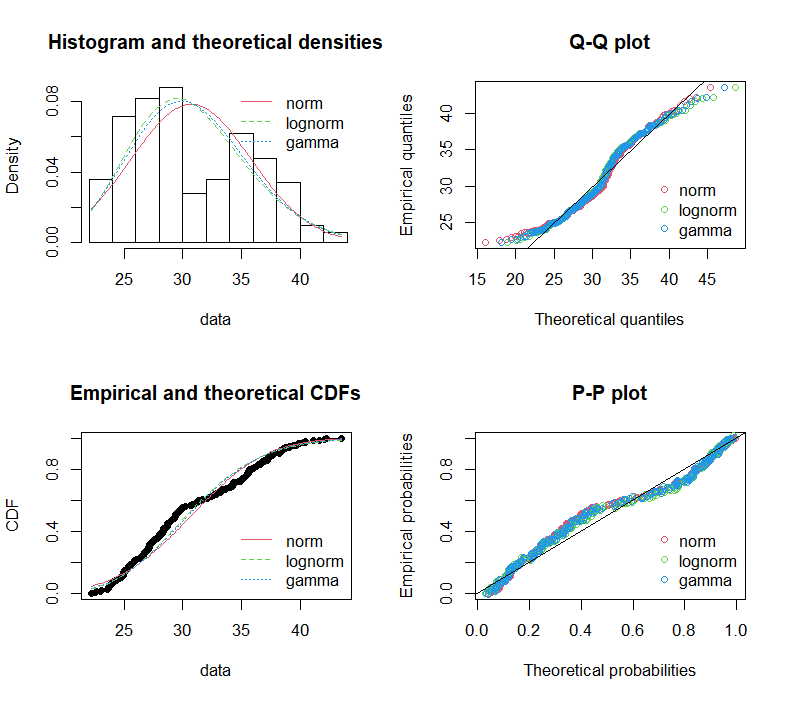
\includegraphics[width=12cm, height=12cm]{img/Wykresy_diagnostyczne_WMG.png}
\caption{Wykresy diagnostyczne - WMG.US}
\end{figure}

\textbf{Rozkłady prawdopodobieństwa} naniesione na histogram gęstości danych. Wykres przedstawia trzy rozkłady teoretyczne (normalny, log-normalny, gamma) dopasowane parametrami do histogramu gęstości danych. 

\textbf{Wykres kwantylowy QQ-plot} to graficzne narzędzie, które porównuje rozkłady prawdopodobieństwa przez wykreślenie ich kwantyli na przeciwnych osiach (x,y). W przypadku, gdy dane są zgodne z danym rozkładem teoretycznym, punkty na wykresie układają się wzdłuż prostej \(y = x\).

\textbf{CDF}, czyli \textbf{Cumulative Distribution Function} (Dystrybuanta), to funkcja rzeczywista wyznaczająca rozkład prawdopodobieństwa. Przyporządkowuje każdej możliwej wartości zmiennej losowej pewne prawdopodobieństwo, że ta wartość jest mniejsza lub równa danej liczbie. Maksymalnie dystrybuanta wynosi 1 a minimalnie 0. CDF określa, jak prawdopodobieństwo rozkłada się względem konkretnych wartości zmiennych losowych.

\textbf{Wykres PP-plot} to narzędzie, które działa na podobnej zasadzie co QQ-plot, z tą różnicą, że zamiast kwantyli porónywane są prawdopodobieństwa kumulacyjne, czyli dystrybuanty; empiryczna i teoretyczna. W przypadku, gdy dane są zgodne z danym rozkładem teoretycznym, punkty na wykresie układają się wzdłuż prostej \(y = x\).

Wykresy diagnostyczne w kontekście statystyki i analizy danych służą do oceny adekwatności dopasowania modelu do danych i do znalezienia potencjalnych problemów określonego rozkładu.

Na powyższych wykresach widać, że wykresy przedstawiają się podobnie. Dla histogramu i P-P plot najlepiej przedstawia się rozkład log-normalny. Dla Q-Q plot - rozkład normalny. Natomiast dla wykresu dystrybuanty - rozkład gamma. W celu jednoznacznego określenia, który z rozkładów najbardziej pokrywa się z cenami spółki WMG.US wykorzystam analizę statystyk KS, CM i AD oraz kryteriów informacyjnych AIC i BIC

\vspace*{0.5cm}

\textbf{Analiza matematyczna}

Statystyki te służą do sprawdzania, czy dane zgadzają się z rozkładami: normalnym, log-normalnym i gamma, poprzez analizę różnic między empiryczną dystrybuantą danych a dystrybuantą rozkładów teoretycznych.

Za pomocą tych statystyk możemy precyzyjniej określić, który rozkład najlepiej odpowiada danym, porównując je dla różnych rozkładów w ramach każdej statystyki. Wybieramy ten rozkład, który charakteryzuje się najmniejszą wartością statystyki testowej w większości przypadków, co oznacza, że jego dystrybuanta jest najbardziej zbliżona do empirycznej dystrybuanty danych.

Test \textbf{Kołmogorowa-Smirnowa} jest oparty o największą odległość pomiędzy dystrybuantami empiryczną \(F_n\) i teoretyczną \(F\)

Statystyka \textbf{Craméra-von Misesa} pozwala na ocenę, na ile dane empiryczne zgadzają się z przyjętym teoretycznym rozkładem na przestrzeni całego rozkładu, a nie jak w przypadku KS - punktowej wartości maksymalnej

Test \textbf{Andersona-Darlinga} jest oparty o ważoną odległość Cramera von Misesa pomiędzy dystrybuantami empiryczną \(F_n\) i teoretyczną \(F\) z wagami odpowiadającymi odwrotności wariancji dystrybuanty empirycznej

\vspace*{0.5cm}
\centerline{Statystyki:}
\vspace*{0.2cm}
\centerline{\begin{tabular}{|l|c|c|c|}
\hline
& r. normalny & r. log-normalny & r. gamma  \\
\hline
KS & 0.113 & 0.085 & 0.095  \\
\hline
CM & 0.822 & 0.605 & 0.666  \\
\hline
AD & 4.567 & 3.467 & 3.760  \\
\hline
\end{tabular}}

\vspace*{0.5cm}
\centerline{Kryteria informacyjne:}
\vspace*{0.2cm}

\centerline{\begin{tabular}{|l|c|c|c|}
\hline
& r. normalny & r. log-normalny & r. gamma  \\
\hline
AIC & 1533.568 & 1520.641 & 1523.555  \\
\hline
BIC & 1540.619 & 1527.692 & 1530.606  \\
\hline
\end{tabular}}

\vspace*{1cm}

\newpage
Analizując podane statystyki i kryteria informacyjne, wyniki wskazują, że najniższe wartości statystyk są dla rozkładu log-normalnego, czyli jest on najlepszym modelem opisującym kursy zamknięcia. W każdym kryterium informacyjnym, rozkład log-normalny również osiąga najniższe wartości. Oznacza to, że zdecydowanie ma on najlepsze dopasowanie do danych kursów zamknięcia.


\subsubsection{Hipoteza o równości rozkładów}
Następnym przedmiotem analizy dotyczącym spółki WMG.US jest badanie hipotezy o równości rozkładów. Test Kołmogorowa-Smirnowa (KS) jest używany do porównania dwóch rozkładów prawdopodobieństwa i określenia, jaka jest maksymalna odległość między tymi rozkładami na podanych danych. Przedsawione poniżej są wyniki tego testu wraz z histogramem gęstości wyników testu KS przeprowadzonego 10000 razy na próbkach 100 elementowych generowanych z rozkładu log-normalnego opisującego według hipotezy zerowej ceny spółki WMG.US.
\begin{figure}[h]
\centering
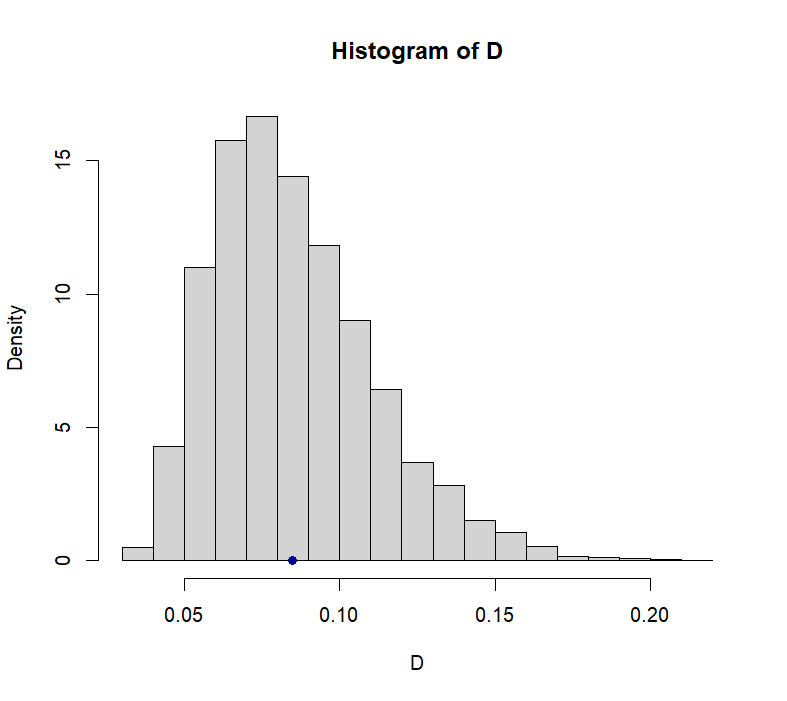
\includegraphics[width=12cm, height=11cm]{img/Histogram_of_D_WMG.png}
\caption{Histogram gęstości wyników testu KS próbek metody Monte-Carlo - WMG.US}
\end{figure}

Hipoteza zerowa \(H_0\) zakłada, że za pomocą rozkładu log-normalnego(o parametrze 3.41) można opisywać ceny spółki WMG.US. Hipoteza alternatywna \(H_1\) ma przeciwne założenia: za pomocą rozkładu log-normalnego (o parametrze 3.41) nie można opisywać cen WMG.US.

Metoda Monte-Carlo, którą testujemy hipotezę zerową polega na wielokrotnym (w tym przypadku 10000-krotnym) generowaniu próbek n-elementowych (tutaj: n=100) z określonego rozkładu  (log-normalny(3.41)), a następnie poddaniu każdorazowo próbki określonemu testowi (KS). 

P-value, czyli procent danych otrzymanych metodą MC, które są większe od testu KS dla oryginalnych danych wynosi 44\%. Test sugeruje, że na danym poziomie istotności, wynoszącym 5\% nie ma podstaw do odrzucenia hipotezy zerowej, zakładającej, że badane dane mają rozkład log-normalny.


\newpage
\subsection{Spółka 11 Bit}
W tym rozdziale przechodzimy do analizy cen akcji spółki 11 Bit Studios. Pierwszym krokiem będzie przyjrzenie się statystykom opisowym.
\subsubsection{Wykres kursów zamknięcia i histogram}
Poniżej znajdują się wykres kursów zamknięcia pokazujący zmiany w czasie oraz histogram dla cen spółki 11 Bit Studios

\begin{figure}[h]
\centering
\begin{minipage}[b]{0.40\textwidth}
\centering
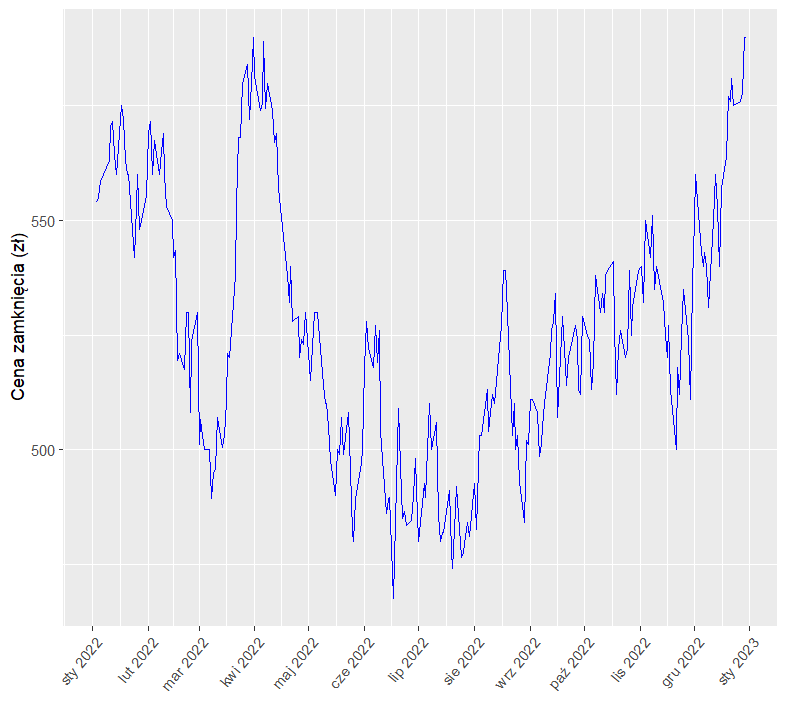
\includegraphics[width=\textwidth, height=5.2cm, width = 7cm]{img/Wykres_cen_akcji_11B.png}
\caption{Wykres cen akcji na zamknięcie dnia przez rok 2022 - 11B}
\label{fig:r3}
\end{minipage}
\hfill
\begin{minipage}[b]{0.40\textwidth}
\centering
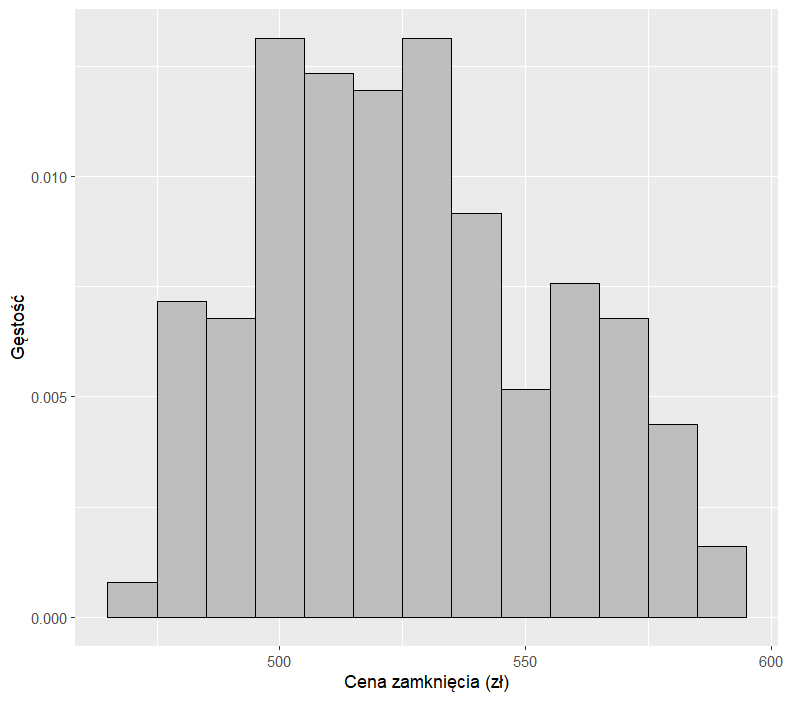
\includegraphics[width=\textwidth, height=5.25cm, width = 7cm]{img/Histogram_kursu_zamkniecia_11B.png}
\caption{Histogram cen zamknięcia - 11B}
\label{fig:r4}
\end{minipage}
\end{figure}

\subsubsection{Statystyki opisowe}
W celu lepszego zrozumienia charakterystyki danych, poniżej są przedstawione podstawowe statystyki opisowe. Te liczby stanowią podsumowanie rozkładu wartości w danej kategorii i pozwalają lepiej zrozumieć centralne tendencje oraz rozbieżności.

\vspace*{0.2cm}
\centerline{\begin{tabular}{|c|c|c|c|c|}
\hline
 & $\bar{x}$ & odch. st. & skośność & kurtoza \\
\hline
Akcja & 536.20 & 29.16 & 0.28 & -0.82 \\
\hline
\end{tabular}}

\vspace*{0.5cm}

Interpretacja statystyk:
\begin{itemize}
    \item Dane są skupione wokół średniej równej 536,20.

    \item Odchylenie standardowe mierzy, jak bardzo dane są rozproszone wokół średniej. Im wyższa wartość odchylenia standardowego, tym większa zmienność danych. W tym przypadku 29,16 wskazuje na pewną rozbieżność danych wokół średniej.

    \item Wartość dodatnia (0,28) sugeruje, że rozkład może być nieco przesunięty w prawo (więcej wartości skrajnych po prawej stronie średniej). Jednak skośność ta jest bliska zeru, co oznacza, że asymetria jest niewielka.

    \item Wartość ujemna (-0,82) wskazuje na lekko spłaszczony rozkład w porównaniu do rozkładu normalnego.

\end{itemize}

Podsumowując, analiza statystyczna wskazuje na to, że dane mają średnią wartość 536,20, są nieco rozproszone wokół średniej (odchylenie standardowe 29,16), mają niewielką asymetrię w prawo (skośność 0,28) i lekko spłaszczone ogony w porównaniu do rozkładu normalnego (kurtoza -0,82).

\subsubsection{Esytymacja parametrów trzech rozkładów}
W celu pełniejszego zrozumienia charakterystyki danych, można przeprowadzić estymację parametrów trzech różnych rozkładów: rozkładu normalnego, log-normalnego oraz gamma.

\vspace*{0.2cm}
\centerline{\begin{tabular}{|c|cc|cc|cc|}
\hline
& \multicolumn{2}{c|}{\textbf{r. normalny}} 
& \multicolumn{2}{c|}{\textbf{r. log-normalny}}                        
& \multicolumn{2}{c|}{\textbf{r. gamma}} \\ \hline
parametr & mean & sd & meanlog & sdlog & shape & rate \\ \hline
estimate & 526,20 & 29,10 & 6,26 & 0,06 & 329,61 & 0,63 \\ \hline
std. error & 1,84 & 1,30 & 0,003 & 0,002 & 29,38 & 0,06 \\ \hline
\end{tabular}}



Analizując przedstawione wyniki estymacji dla trzech różnych rozkładów (to znaczy; normalny, log-normalny oraz gamma), można uzyskać istotne informacje dotyczące charakterystyki badanych danych.
\begin{description}
    \item[Rozkład normalny] Dane wydają się być skoncentrowane wokół średniej 526,20, a odchylenie standardowe 29,10 wskazuje na pewną zmienność, ale nie jest ona zbyt duża. To sugeruje, że dane mają kształt zbliżony do rozkładu normalnego.
    \item[Rozkład log-normalny] Niskie odchylenie standardowe logarytmiczne 0,06 sugeruje, że dane mogą mieć tendencję do skupiania się wokół pewnej wartości centralnej.
    \item[Rozkład gamma] E(x) w tym wypadku wynosi 526,19, który to wynik jest bardzo zbliżony do średnij z rozkładu normalnego. Wysoki kształt i stosunkowo niskie tempo sugerują, że dane są zróżnicowane z dłuższymi ogonami.
\end{description}


\subsubsection{Analiza statystyk}
\textbf{Analiza wzrokowa}

Poniżej przedstawiony jest zbiór wybranych wykresów diagnostycznych; histogram z rokładami teoretycznymi, wykres kwantylowy, dystrybuanta i wykres P-P
\begin{figure}[h]
\centering
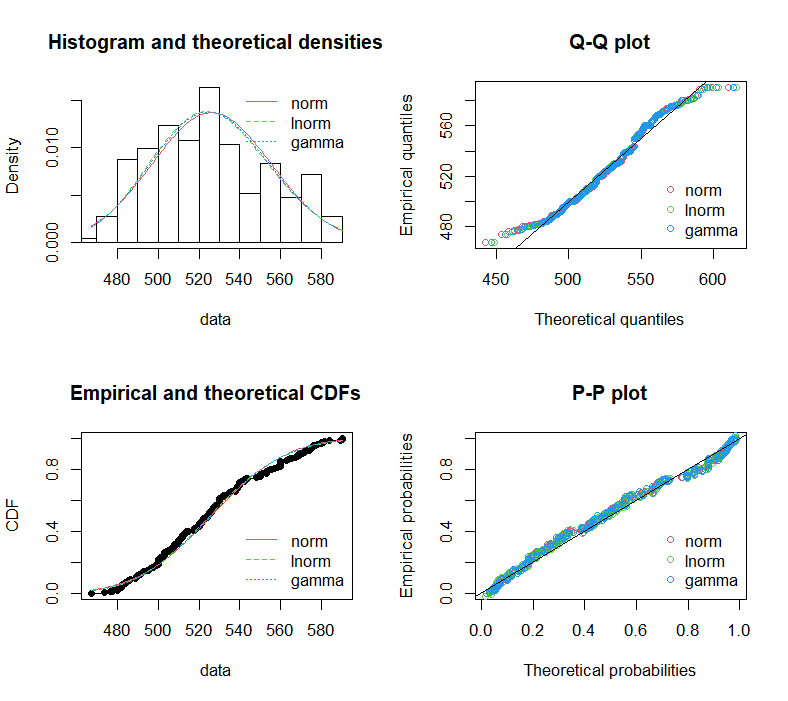
\includegraphics[width=12cm, height=12cm]{img/Wykresy_diagnostyczne_11B.png}
\caption{Wykresy diagnostyczne - 11B}
\end{figure}

\textbf{Rozkłady prawdopodobieństwa} naniesione na histogram gęstości danych. Wykres przedstawia trzy rozkłady teoretyczne (normalny, log-normalny, gamma) dopasowane parametrami do histogramu gęstości danych. 

\textbf{Wykres kwantylowy QQ-plot} to graficzne narzędzie, które porównuje rozkłady prawdopodobieństwa przez wykreślenie ich kwantyli na przeciwnych osiach (x,y). W przypadku, gdy dane są zgodne z danym rozkładem teoretycznym, punkty na wykresie układają się wzdłuż prostej \(y = x\).

\textbf{CDF}, czyli \textbf{Cumulative Distribution Function} (Dystrybuanta), to funkcja rzeczywista wyznaczająca rozkład prawdopodobieństwa. Przyporządkowuje każdej możliwej wartości zmiennej losowej pewne prawdopodobieństwo, że ta wartość jest mniejsza lub równa danej liczbie. Maksymalnie dystrybuanta wynosi 1 a minimalnie 0. CDF określa, jak prawdopodobieństwo rozkłada się względem konkretnych wartości zmiennych losowych.

\textbf{Wykres PP-plot} to narzędzie, które działa na podobnej zasadzie co QQ-plot, z tą różnicą, że zamiast kwantyli porónywane są prawdopodobieństwa kumulacyjne, czyli dystrybuanty; empiryczna i teoretyczna. W przypadku, gdy dane są zgodne z danym rozkładem teoretycznym, punkty na wykresie układają się wzdłuż prostej \(y = x\).

Wykresy diagnostyczne w kontekście statystyki i analizy danych służą do oceny adekwatności dopasowania modelu do danych i do znalezienia potencjalnych problemów określonego rozkładu.

Analiza graficzna rozkładów kursów zamknięcia nie pozwala jednoznacznie określić, który z rozkładów - normalny, log-normalny czy gamma - najlepiej opisuje dane. Dlatego trzeba wykorzystać dodatkowe statystyki i kryteria informacyjne, takie jak KS (test Kołmogorowa-Smirnowa), CM (test Craméra-von Misesa), AD (test Andersona-Darlinga) oraz kryteria informacyjne AIC i BIC.

\vspace*{0.5cm}
\textbf{Analiza matematyczna}

Statystyki te służą do sprawdzania, czy dane zgadzają się z rozkładami: normalnym, log-normalnym i gamma, poprzez analizę różnic między empiryczną dystrybuantą danych a dystrybuantą rozkładów teoretycznych.

Za pomocą tych statystyk możemy precyzyjniej określić, który rozkład najlepiej odpowiada danym, porównując je dla różnych rozkładów w ramach każdej statystyki. Wybieramy ten rozkład, który charakteryzuje się najmniejszą wartością statystyki testowej w większości przypadków, co oznacza, że jego dystrybuanta jest najbardziej zbliżona do empirycznej dystrybuanty danych.

Test \textbf{Kołmogorowa-Smirnowa} jest oparty o największą odległość pomiędzy dystrybuantami empiryczną \(F_n\) i teoretyczną \(F\)

Statystyka \textbf{Craméra-von Misesa} pozwala na ocenę, na ile dane empiryczne zgadzają się z przyjętym teoretycznym rozkładem na przestrzeni całego rozkładu, a nie jak w przypadku KS - punktowej wartości maksymalnej

Test \textbf{Andersona-Darlinga} jest oparty o ważoną odległość Cramera von Misesa pomiędzy dystrybuantami empiryczną \(F_n\) i teoretyczną \(F\) z wagami odpowiadającymi odwrotności wariancji dystrybuanty empirycznej



\vspace*{0.2cm}
\centerline{Statystyki:}
\vspace*{0.2cm}

\centerline{\begin{tabular}{|l|c|c|c|}
\hline
& r. normalny & r. log-normalny & r. gamma  \\
\hline
KS & 0,0653 & 0,0640 & 0,0643  \\
\hline
CM & 0,2665 & 0,2037 & 0,2228  \\
\hline
AD & 1,863 & 1,503 & 1,612  \\
\hline
\end{tabular}}

\vspace*{0.5cm}
\centerline{Kryteria informacyjne:}
\vspace*{0.2cm}

\centerline{\begin{tabular}{|l|c|c|c|}
\hline
& r. normalny & r. log-normalny & r. gamma  \\
\hline
AIC & 274.74 & 223.55 & 238.35  \\
\hline
BIC & 281.73 & 230.54 & 245.35  \\
\hline
\end{tabular}}

\vspace*{0.5cm}


Analizując podane statystyki i kryteria informacyjne, wyniki wskazują, że najniższe wartości statystyk są dla rozkładu log-normalnego, czyli jest on najlepszym modelem opisującym kursy zamknięcia. W każdym kryterium informacyjnym, rozkład log-normalny również osiąga najniższe wartości. Oznacza to, że zdecydowanie ma on najlepsze dopasowanie do danych kursów zamknięcia.

\newpage
\subsubsection{Hipoteza o równości rozkładów}
Następnym przedmiotem analizy dotyczącym spółki WMG.US jest badanie hipotezy o równości rozkładów. Test Kołmogorowa-Smirnowa (KS) jest używany do porównania dwóch rozkładów prawdopodobieństwa i określenia, jaka jest maksymalna odległość między tymi rozkładami na podanych danych.

Hiptotezą zerową jest, że dystrybuanty \(F\) i \(F0\) są równe, to znaczy, brak istotnej różnicy pomiędzy dystrybuantą empiryczną a dystrybuantą teoretyczną. Za poziom istotności, \(\alpha\), najczęściej przyjmuje się 5\%. W tym wypadku jest tylko jedna hipoteza alternatywna, że jednak nie są - \(F \neq F0\).


\begin{figure}[h]
\centering
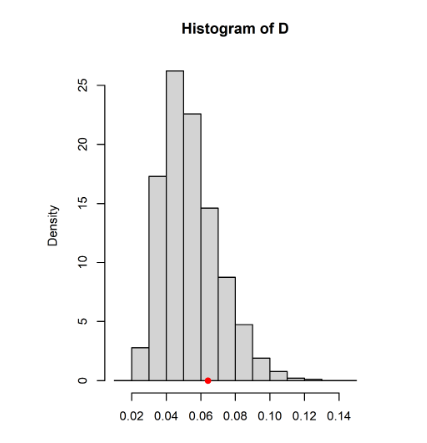
\includegraphics[width=9cm, height=12cm]{img/Histogram_of_D_11B.png}
\caption{ Histogram gęstości wyników testu KS próbek metody Monte-Carlo - 11B}
\end{figure}
Test Kołmogorowa-Smirnowa, służy do weryfikacji hipotezy o nieistotności różnicy badanego rozkładu zmiennej (rozkładu empirycznego) z rozkładem normalnym (rozkładem teoretycznym).

Metoda Monte-Carlo, którą testujemy hipotezę zerową polega na wielokrotnym generowaniu próbek n-elementowych z określonego rozkładu, a następnie poddaniu każdorazowo próbki określonemu testowi (KS).

Na wykresie jako histogram zaznaczona jest gęstość z estymowanych rozkładów na podstawie 10.000 próbek, a w każdej z nich 100 próbek przy prawdopodobieństwie zgodnym z testowanym rozkładem. Czerwonym punktem zaznaczona jest wartość jaką otrzymaliśmy dzięki metodzie KS dla kursów zamknięcia i testowanego rozkładu.

Obliczając ilość danych większych od wartości statystyki testu KS dla oryginalnych danych zostaje otrzymany wynik około 25\%. Test wskazuje, że na danym poziomie istotności nie można odrzucić hipotezy zerowej, o tym, że analizowane dane przedstawiają rozkład log-normalny.


\newpage
\section{Analiza łącznego rozkładu log-zwrotów}
Po analizie każdej ze spółek osobono, następnym zadaniem jest aby porównać je między sobą. Ze względu na różnice w cenach akcji analiza będzie dotyczych logarytmicznych zwrotów (różnic dziennych między cenami danej spółki). Analiza została podzielona na następujące części: rozkłady brzegowe, estymacja parametrów rozkładu dwuwymiarowego normalnego oraz analiza dobroci dopasowania i analiza dopasowania rozkładu normalnego
\subsection{Analiza rozkładów brzegowych}
W kolejnych podrozdziałach opisane zostaną log-zwroty kolejno WMG.US i 11B. Do każdego opisu dołączone zostanie test równości rozkładów metodą MC.
\subsubsection{Log-zwroty spółki WMG.US}
Poniżej przedstawione są wykres oraz histogram log-zwrotów, które dostarczają wizualnej reprezentacji tego rozkładu.

\begin{figure}[h]
\centering
\begin{minipage}[b]{0.45\textwidth}
\centering
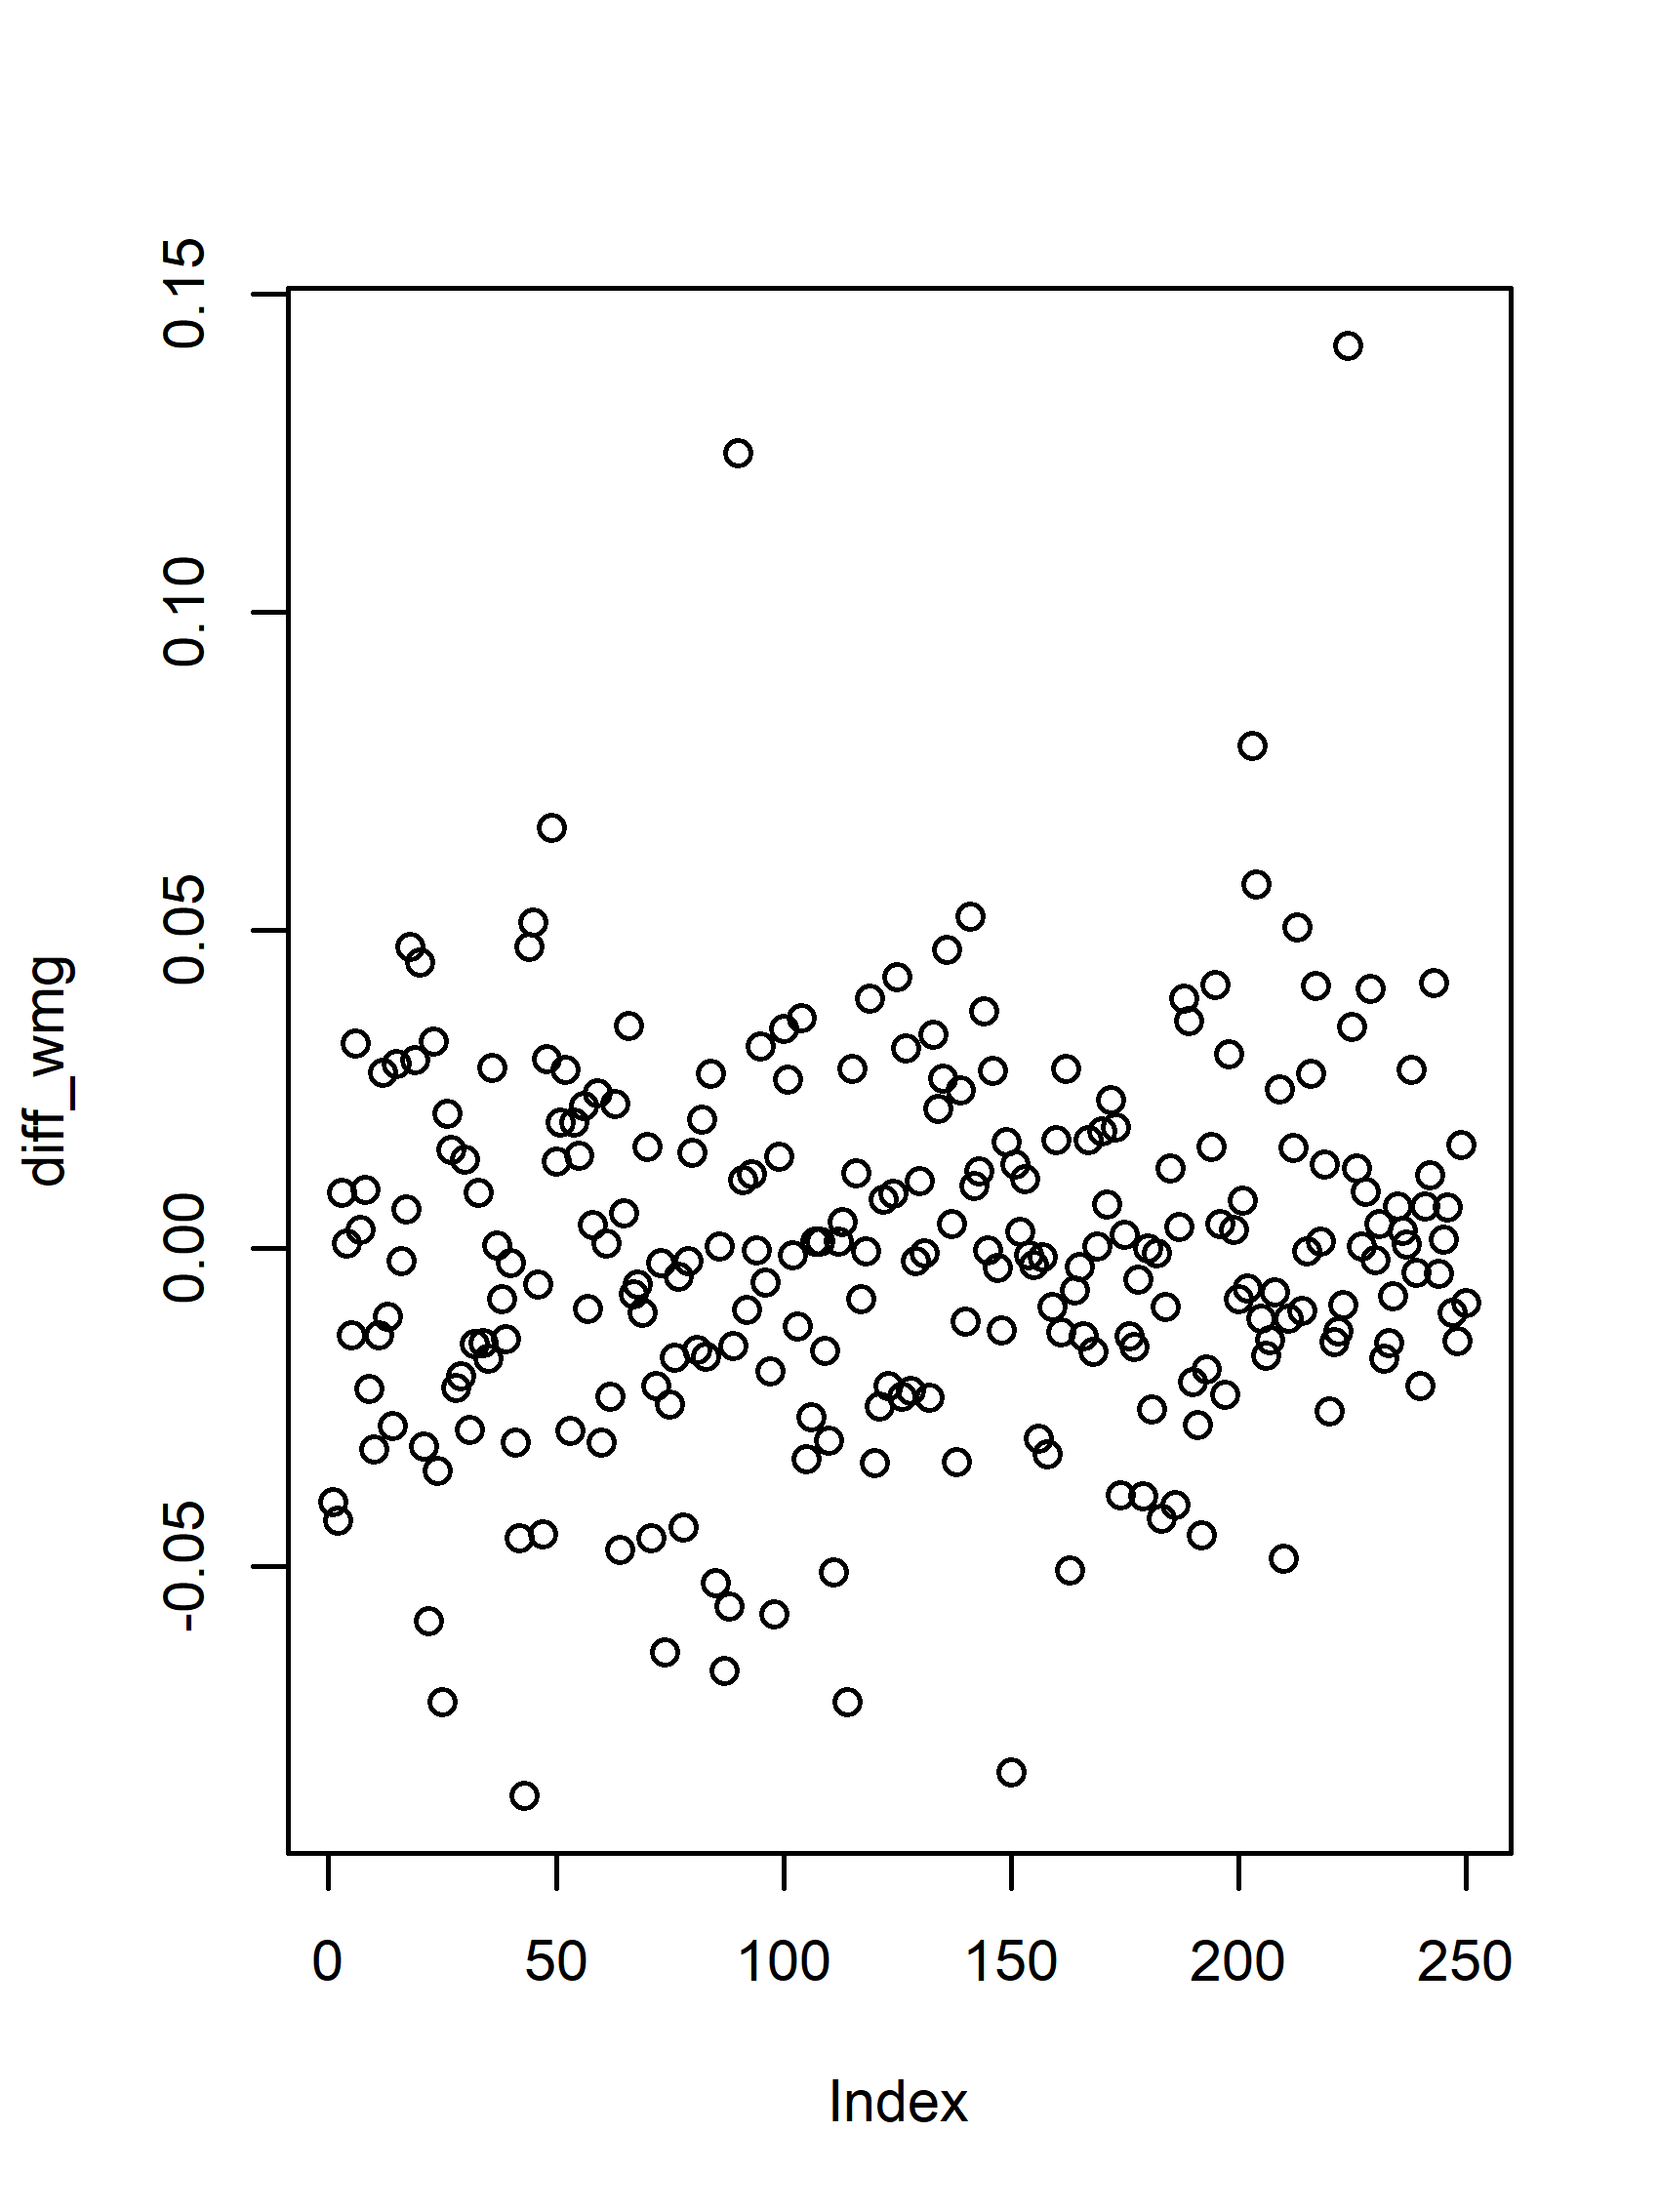
\includegraphics[width=\textwidth, height=7cm, width = 5.25cm]{img/diff_wmg.png}
\caption{Wykres log-zwrotów WMG.US}
\label{fig:r1}
\end{minipage}
\hfill
\begin{minipage}[b]{0.45\textwidth}
\centering
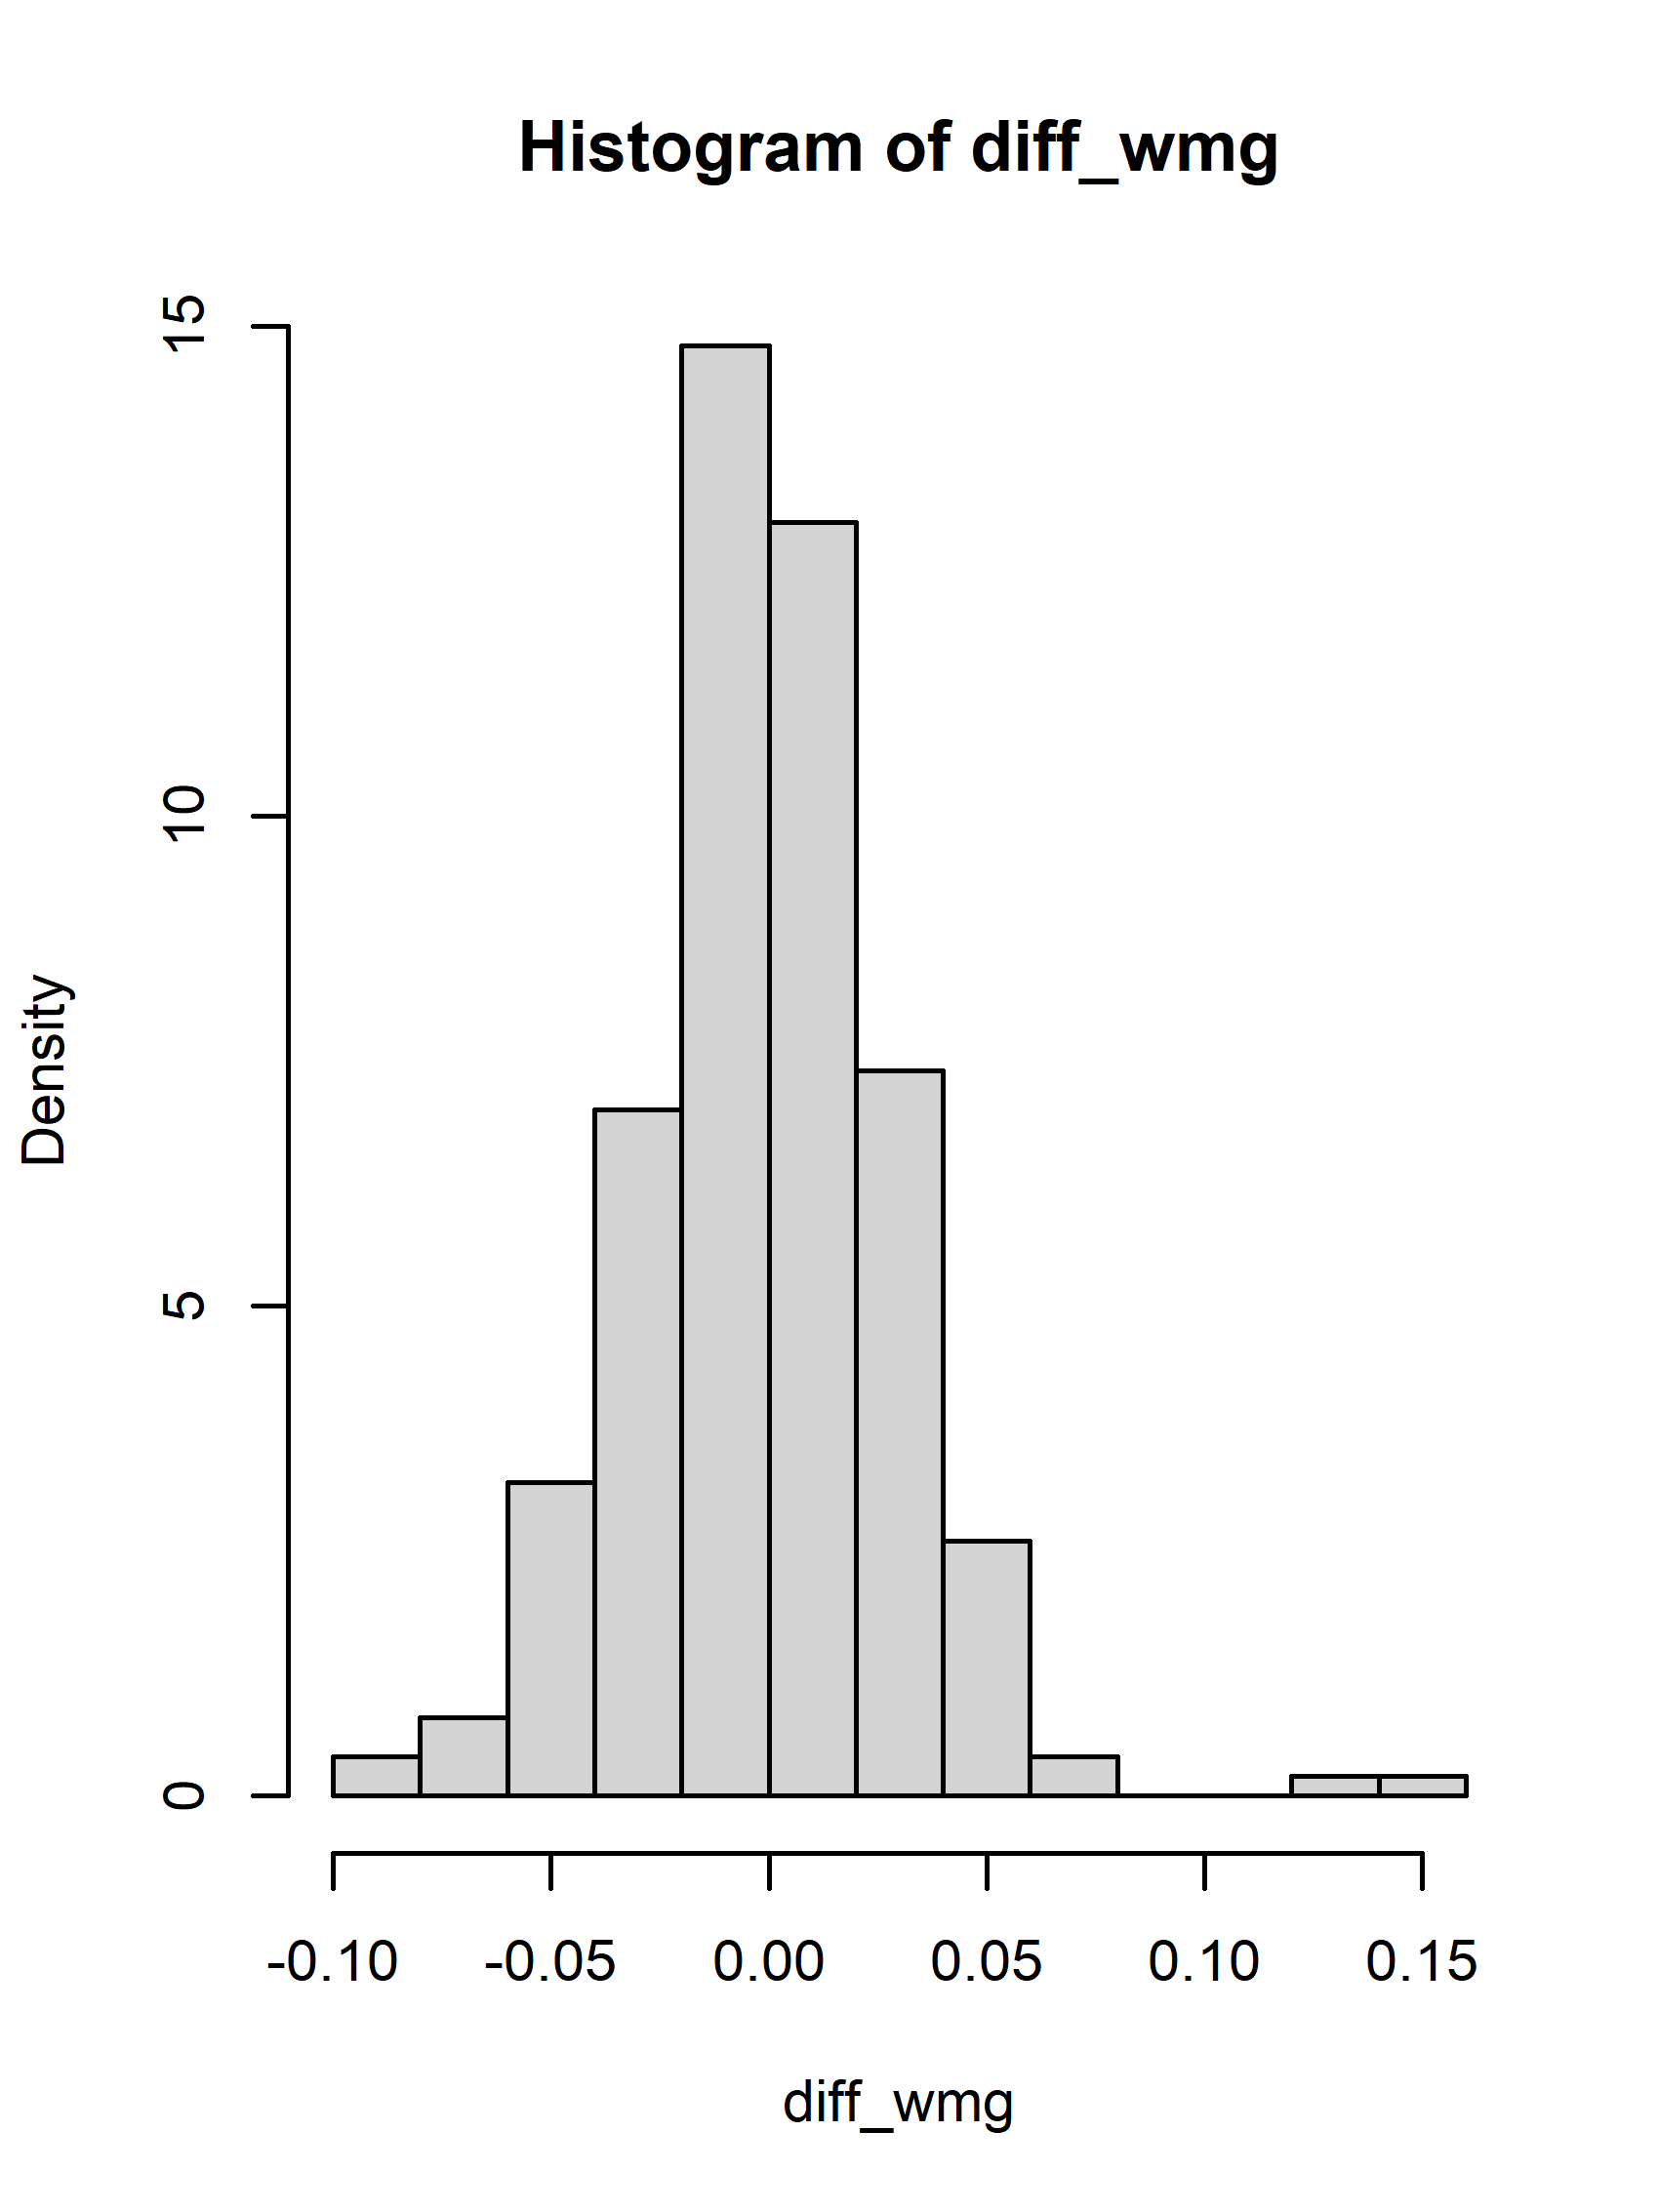
\includegraphics[width=\textwidth, height=7cm, width = 5.25cm]{img/diff_wmg_histogram.png}
\caption{Histogram log-zwrotów WMG.US}
\label{fig:r2}
\end{minipage}
\end{figure}

Z analizy wzrokowej można zuważyc, że przedstawione dane występują w układzie wartości zbliżonym do rozkładu normalnego. 

\newpage
W celu zweryfikowanie tego spostrzeżenia można wykorzystac wykresy diagnostyczne przedstawione poniżej.

\begin{figure}[h]
\centering
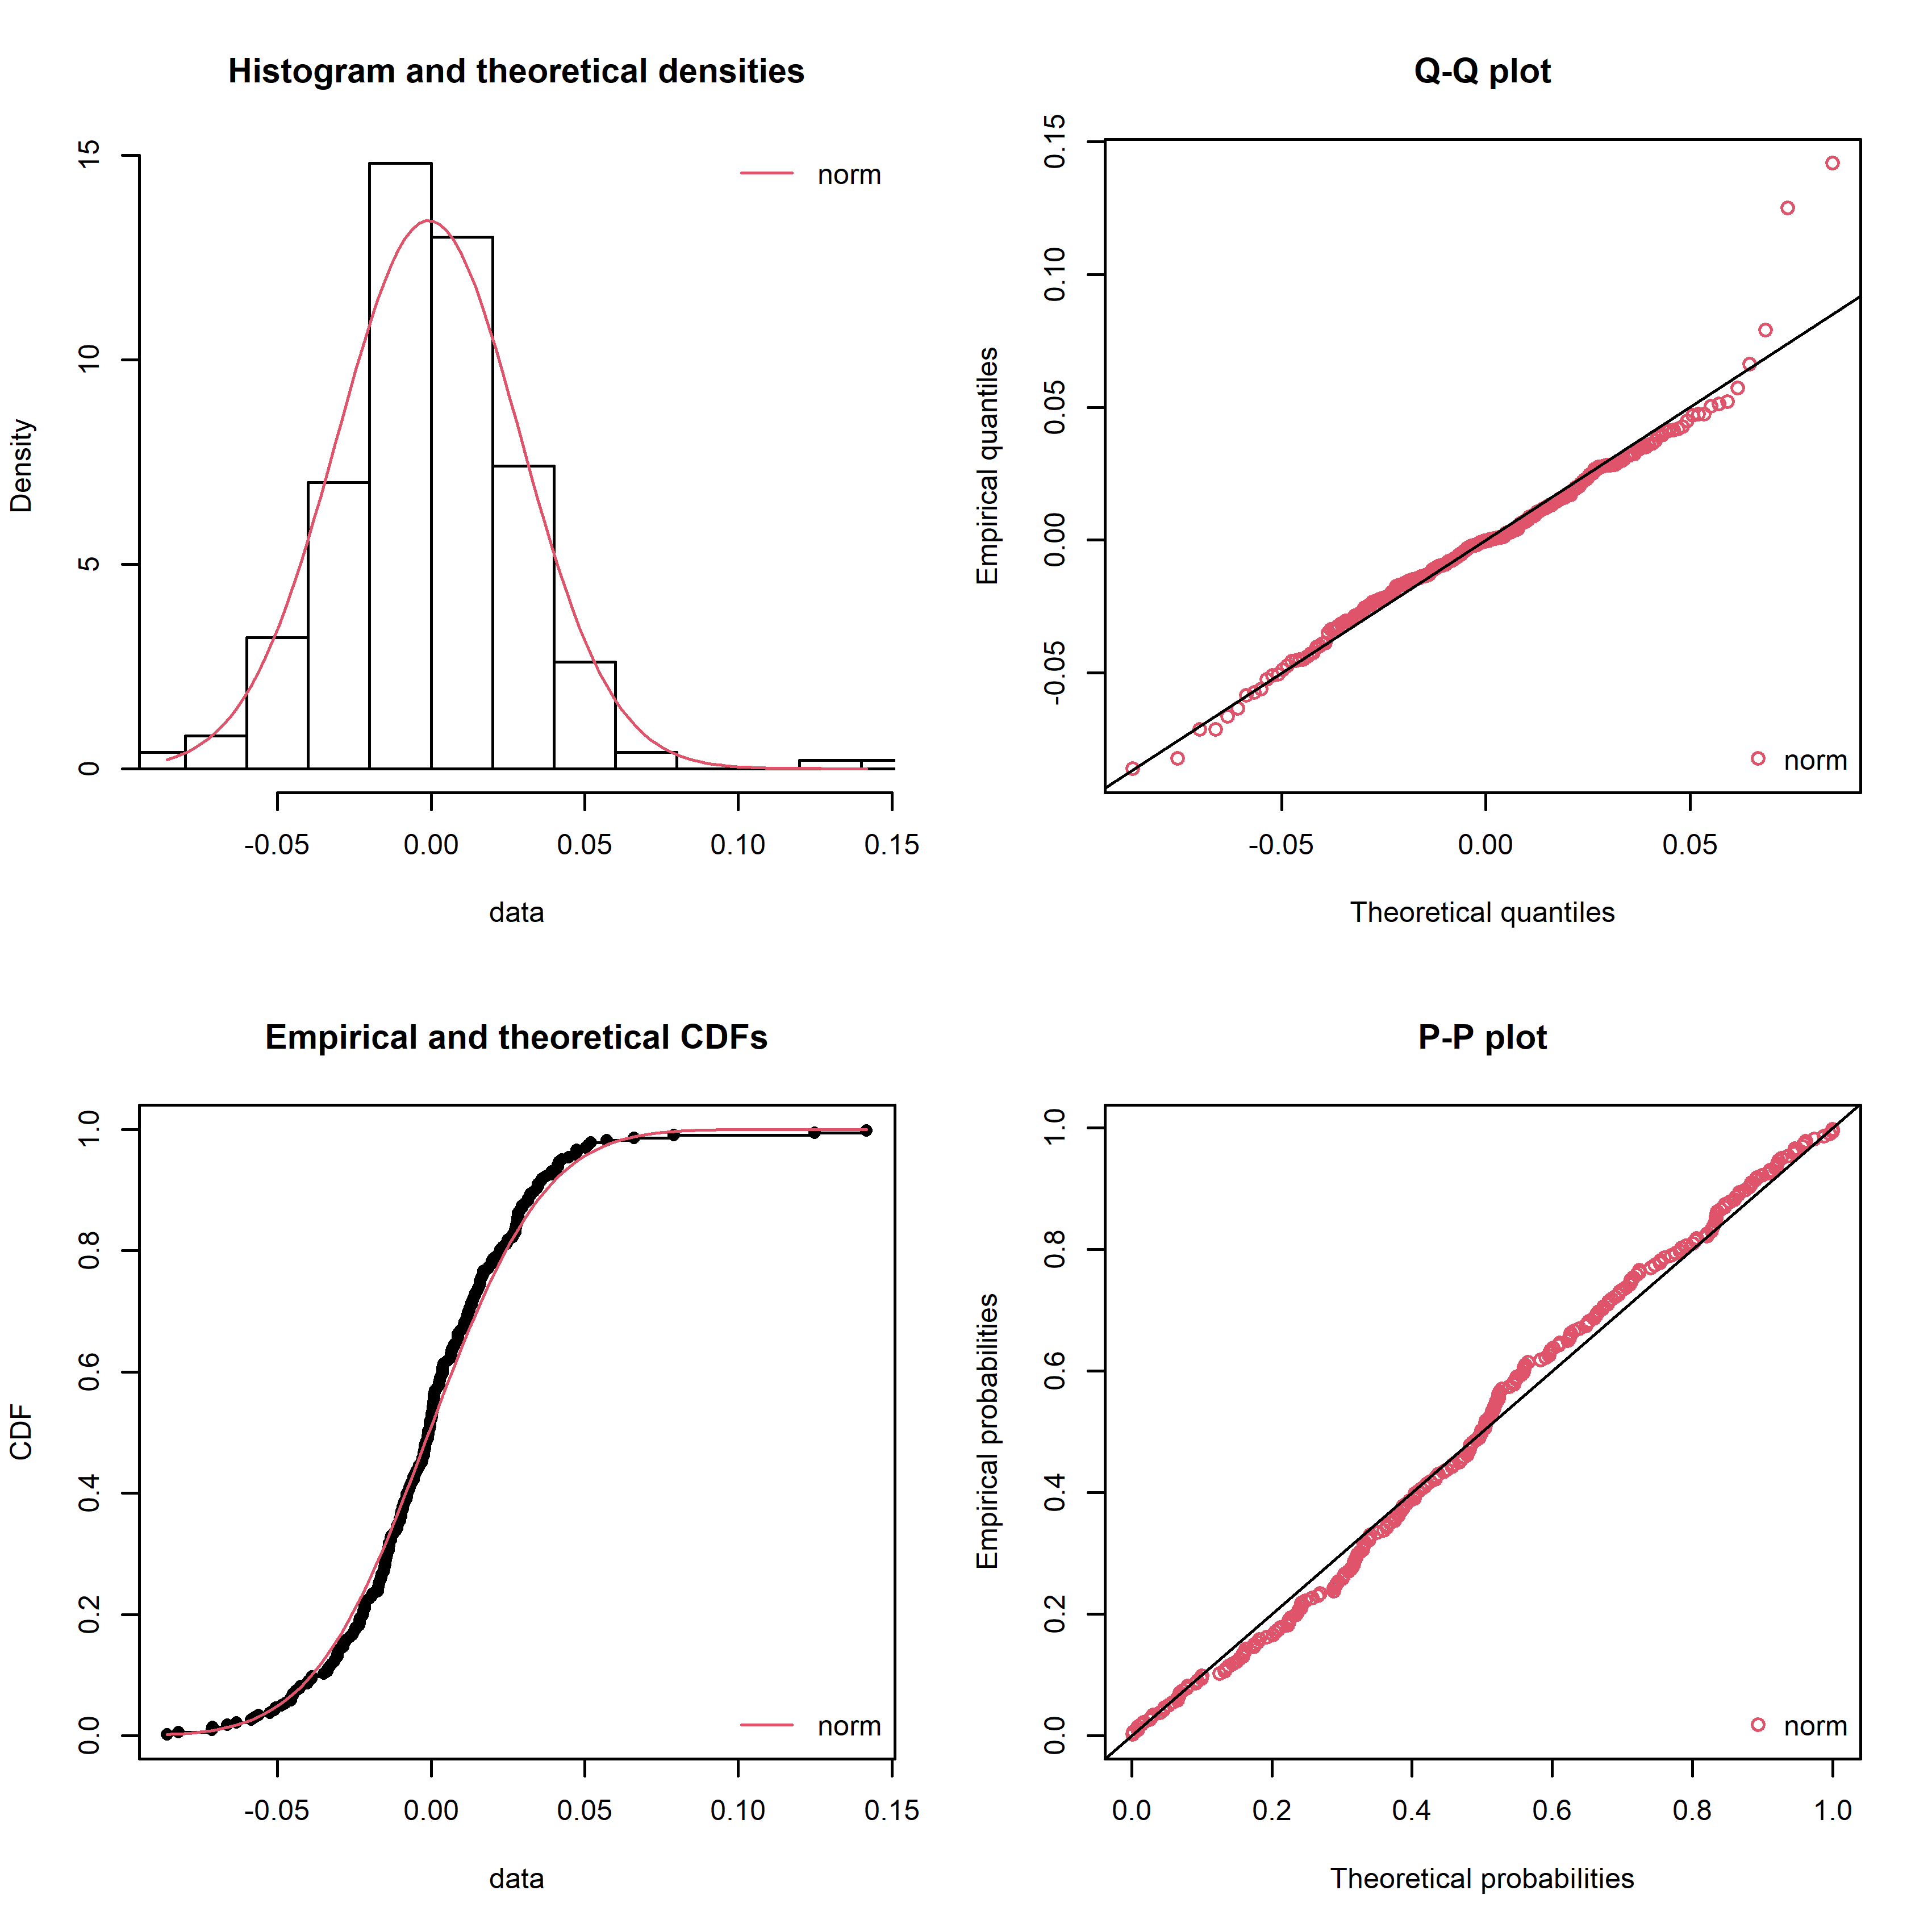
\includegraphics[width=9cm, height=9cm]{img/diff_wmg_wykresy_diagnostyczne.png}
\caption{Wykres diagnostycznie log-zwrotów WMG.US}
\end{figure}

Wykresy diagnostyczne log-zwrotów spółki WMG.US wskazują, że rozkład normalny może pasować do opisywania log-zwrotów tej spółki


\subsubsection{Test równości rozkładów metodą Monte Carlo dla spółki WMG.US}
W kontekście analizy log-zwrotów spółki WMG.US, przeprowadzony został test równości rozkładów z wykorzystaniem metody Monte Carlo. Poniżej zaprezentowany jest histogram z odległością dystrybuanty log-zwrotów oraz wyniki testu statystyki KS, który porównuje badany rozkład z rozkładem normalnym.

\begin{figure}[h]
\centering
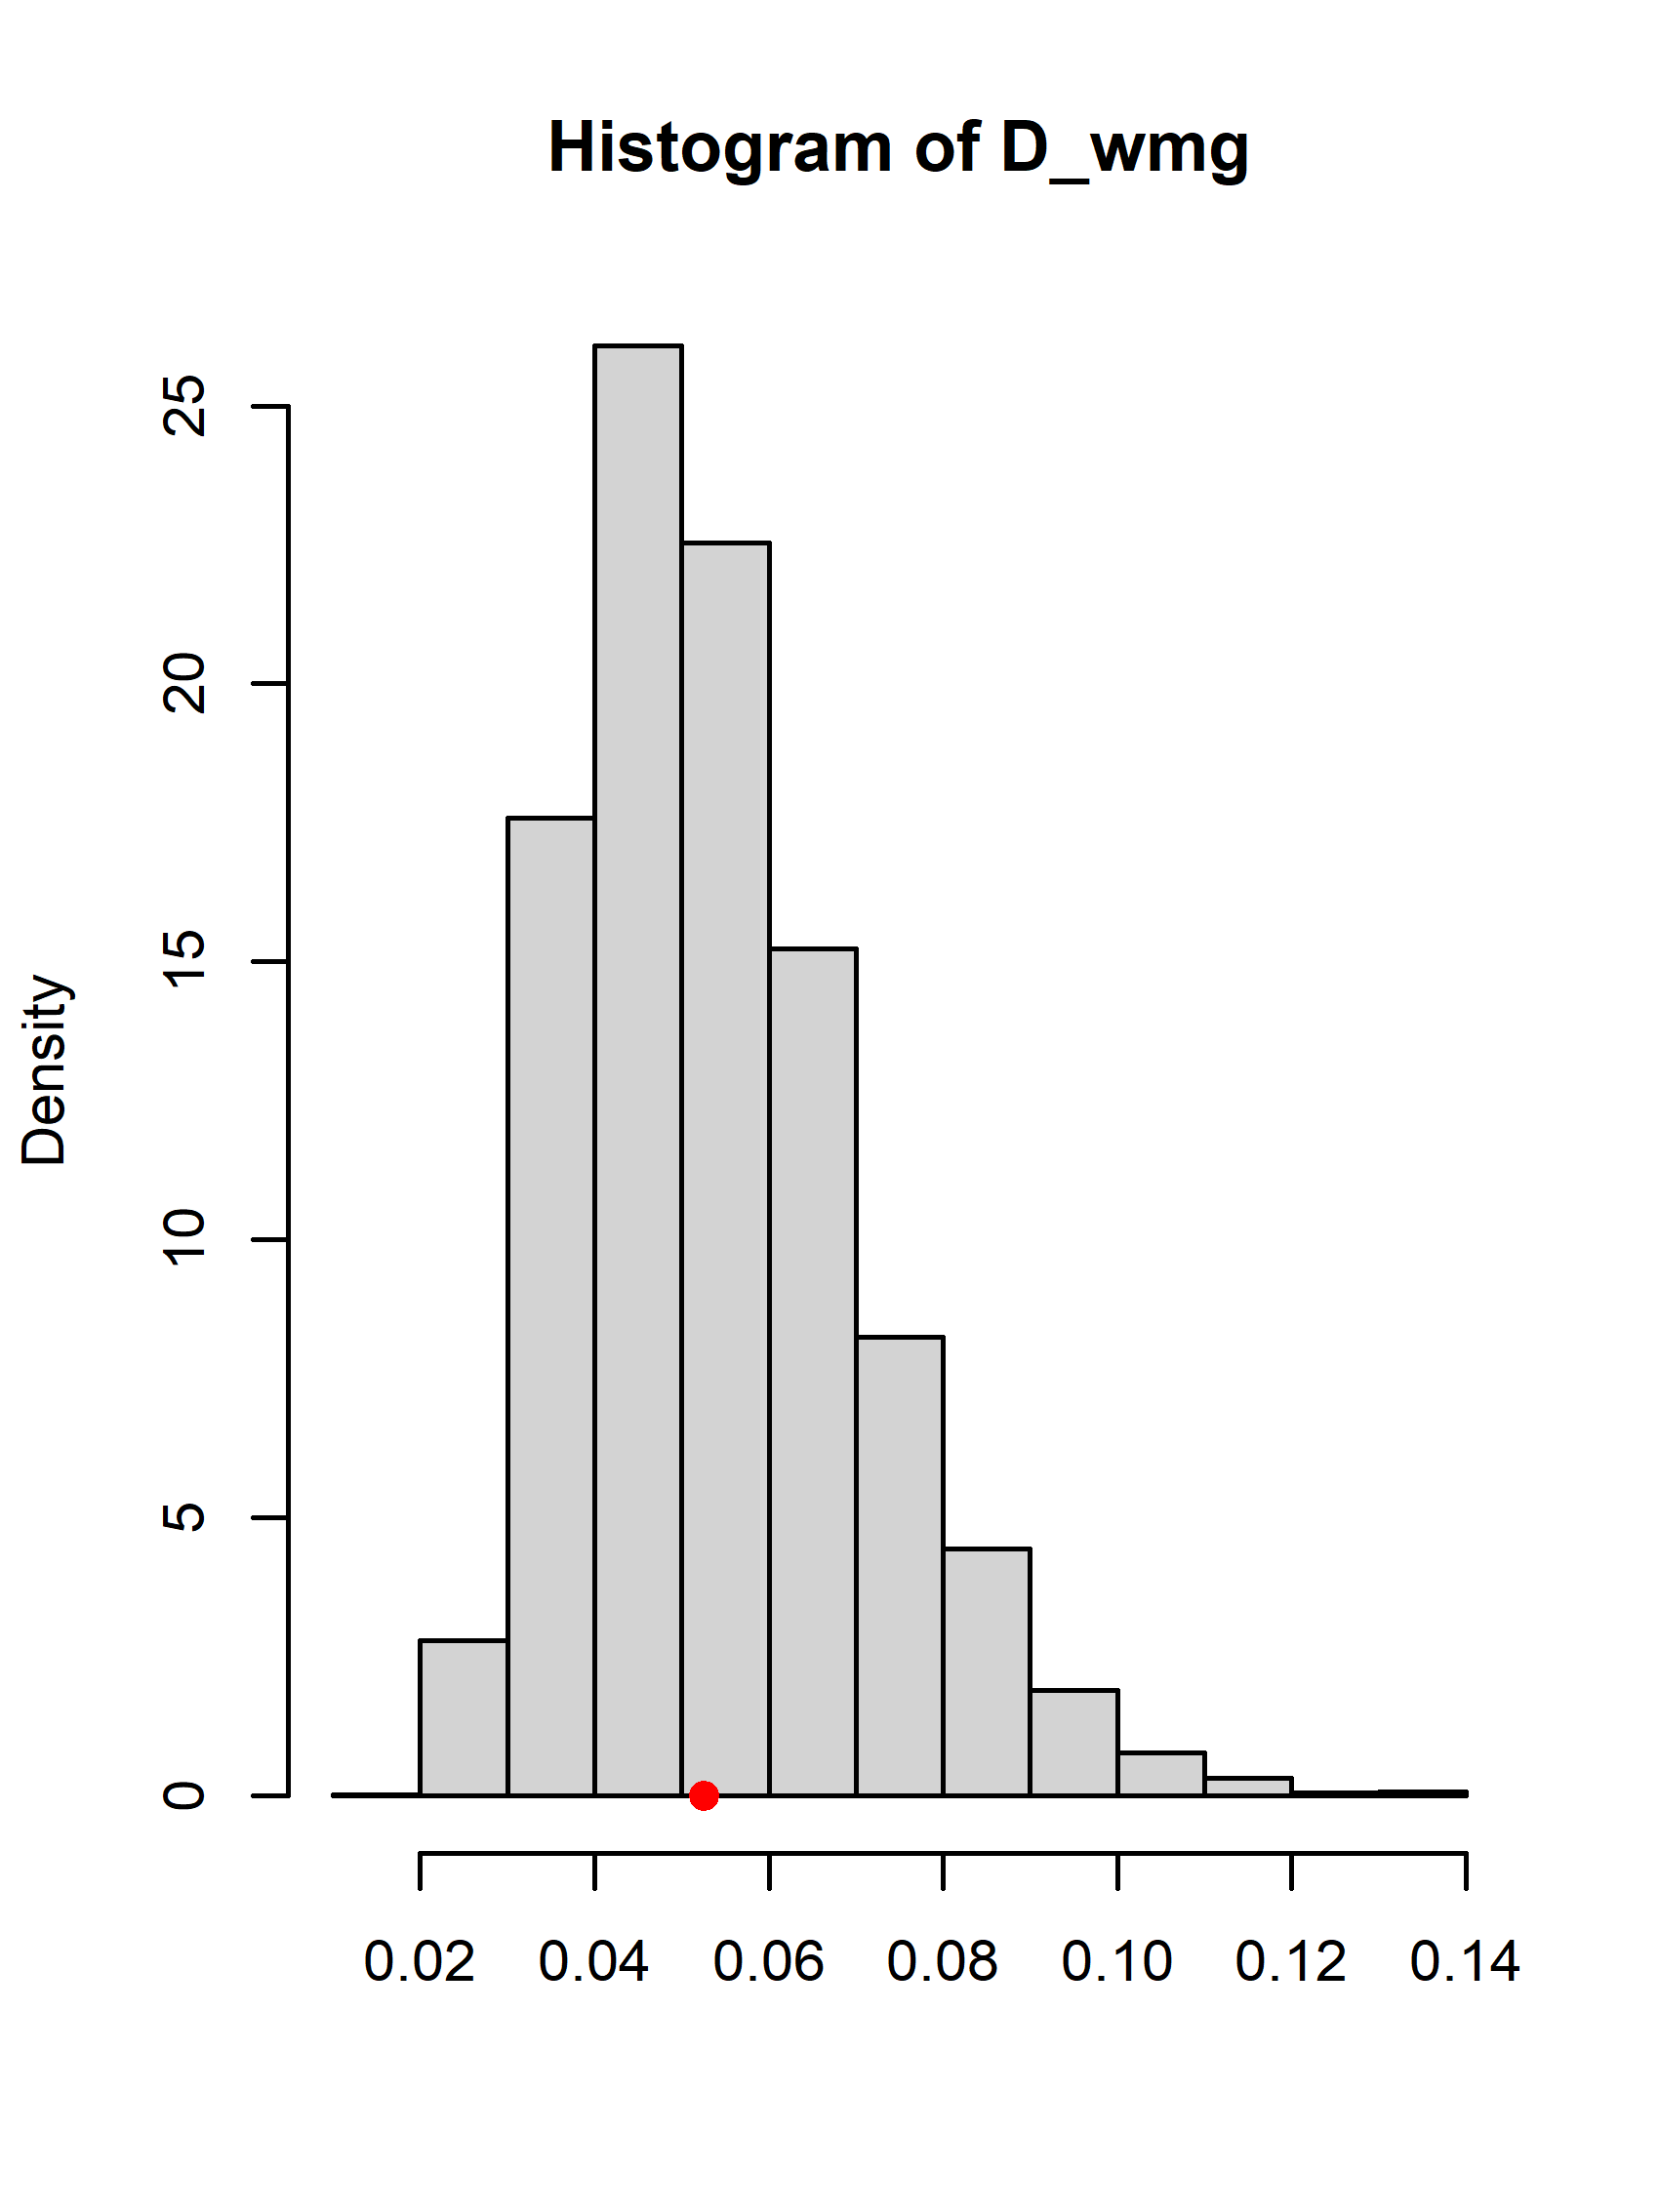
\includegraphics[width=6cm, height=9cm]{img/diff_wmg_hipoteza_o_rownosci.png}
\caption{Histogram gęstości wyników testu KS próbek metody Monte-Carlo WMG.US}
\end{figure}

\newpage
Testowałem rozkład normalny z wykorzystaniem statystyki KS. Wartość p-value wynosi 0.4736, a więc jest znacząco większa od przyjętego poziomu istotności (5\%), czyli nie ma podstaw do odrzucenia hipotezy zerowej, co oznacza, że możemy opisywać dane, czyli log-zwroty spółki WMG.US, za pomocą rozkładu normalnego


\subsubsection{Log-zwroty spółki 11B}
Również dla log-zwrotów spółki 11 Bit Studios przeprowadzona została analiza. Poniżej znajdują się wykresy log-zwrotów oraz histogram, które prezentują wizualną reprezentację tego rozkładu.
\begin{figure}[h]
\centering
\begin{minipage}[b]{0.40\textwidth}
\centering
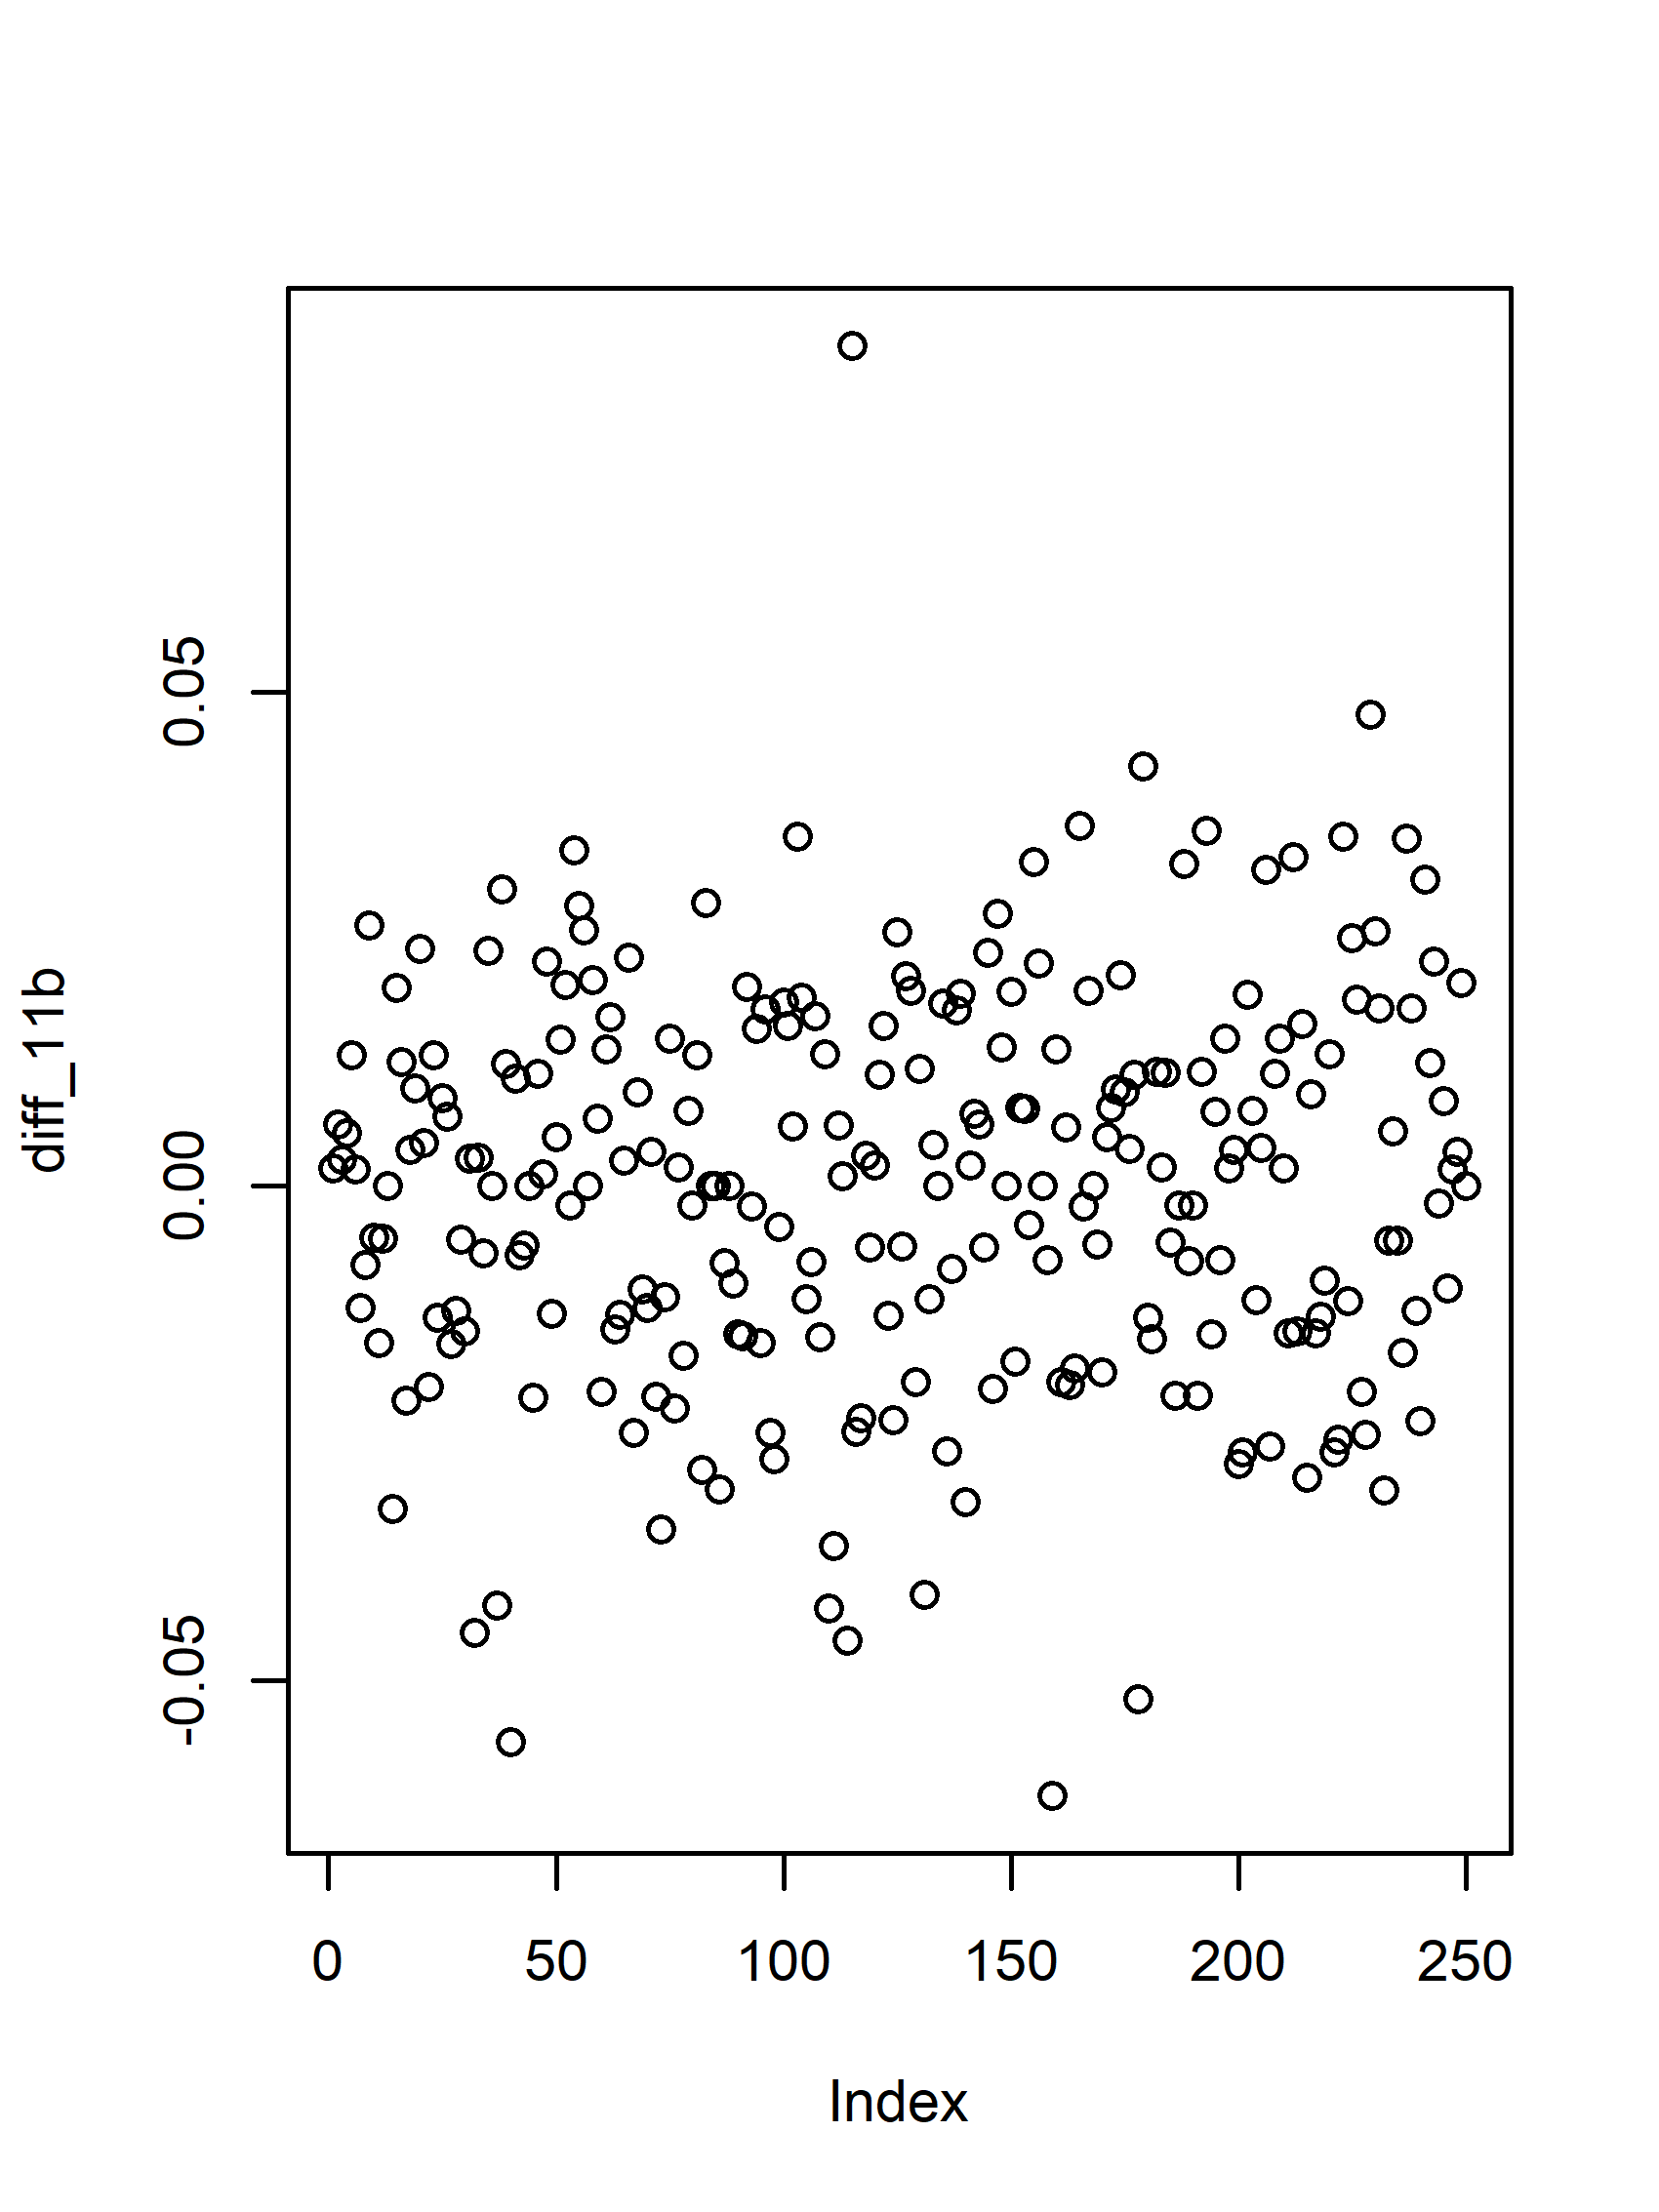
\includegraphics[width=\textwidth, height=7cm, width = 5.25cm]{img/diff_11b.png}
\caption{Wykres log-zwrotów 11B}
\label{fig:r3}
\end{minipage}
\hfill
\begin{minipage}[b]{0.40\textwidth}
\centering
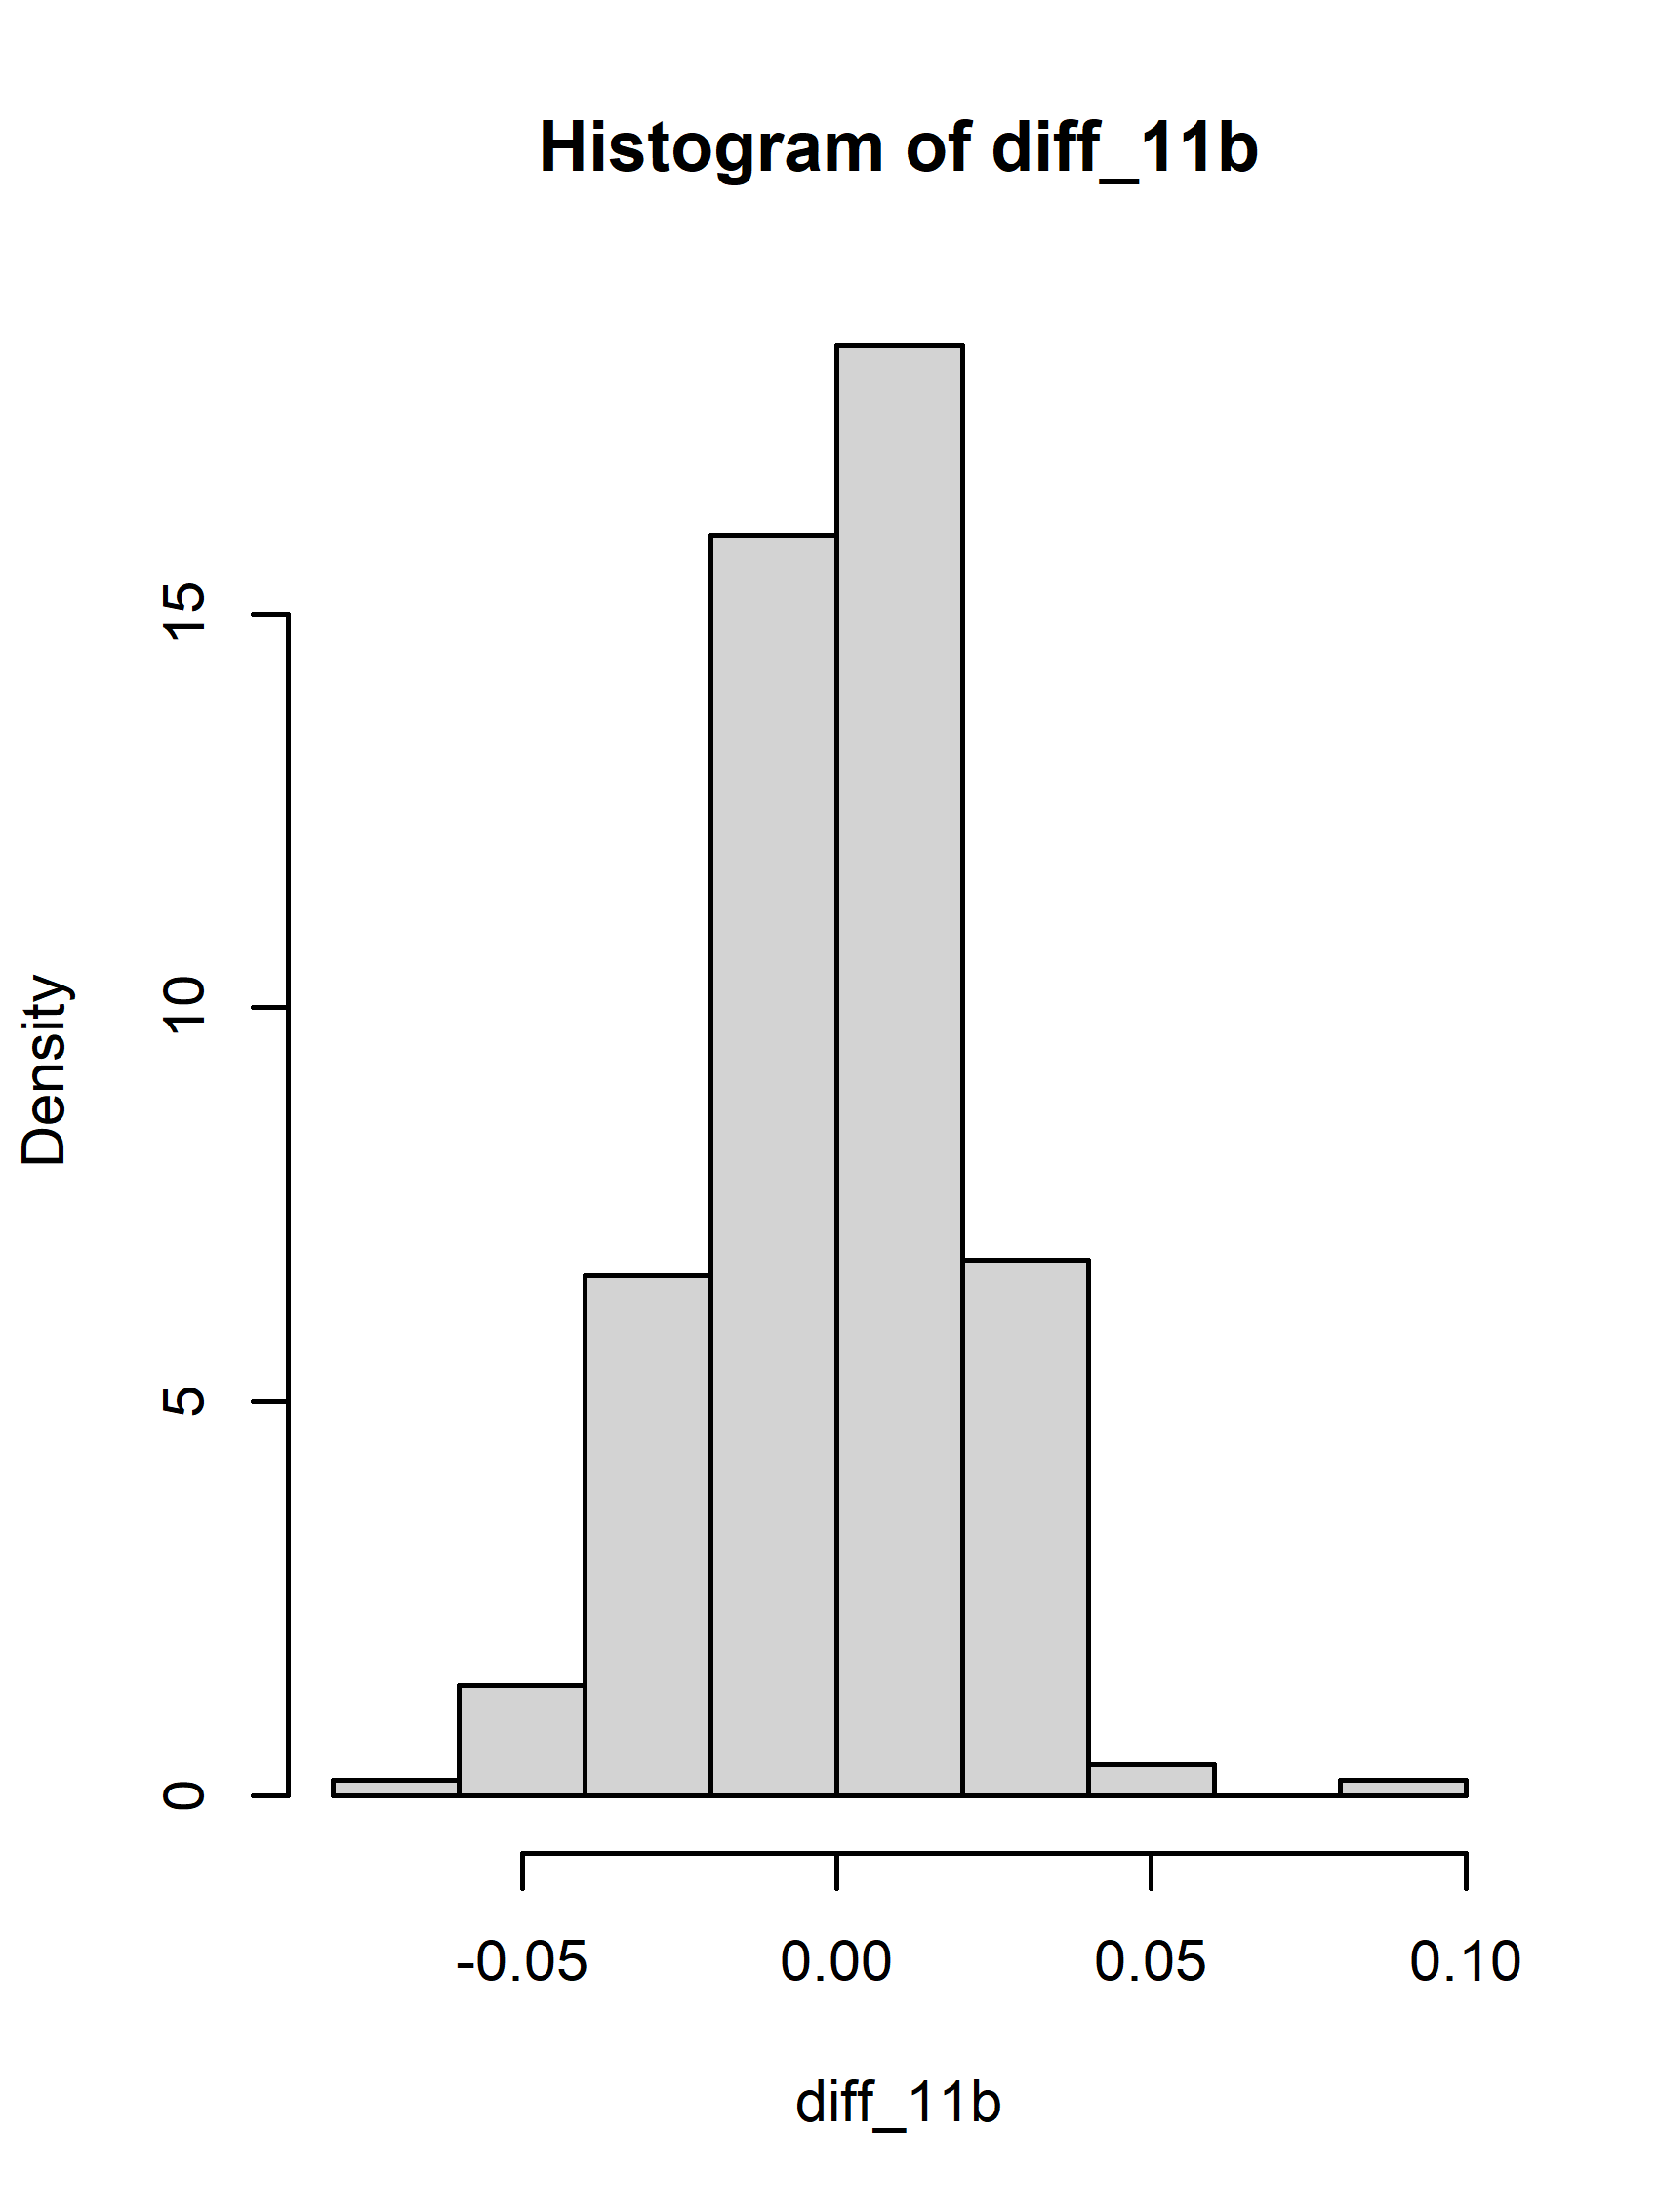
\includegraphics[width=\textwidth, height=7cm, width = 5.25cm]{img/diff_11b_histogram.png}
\caption{Histogram log-zwrotów 11B}
\label{fig:r4}
\end{minipage}
\end{figure}

Z analizy wzrokowej powstaje przypuszczenie, że log-zwroty spółki pasują do rokładu normalnego. Poniżej znajdują się wykresy diagnostyczne

\begin{figure}[h]
\centering
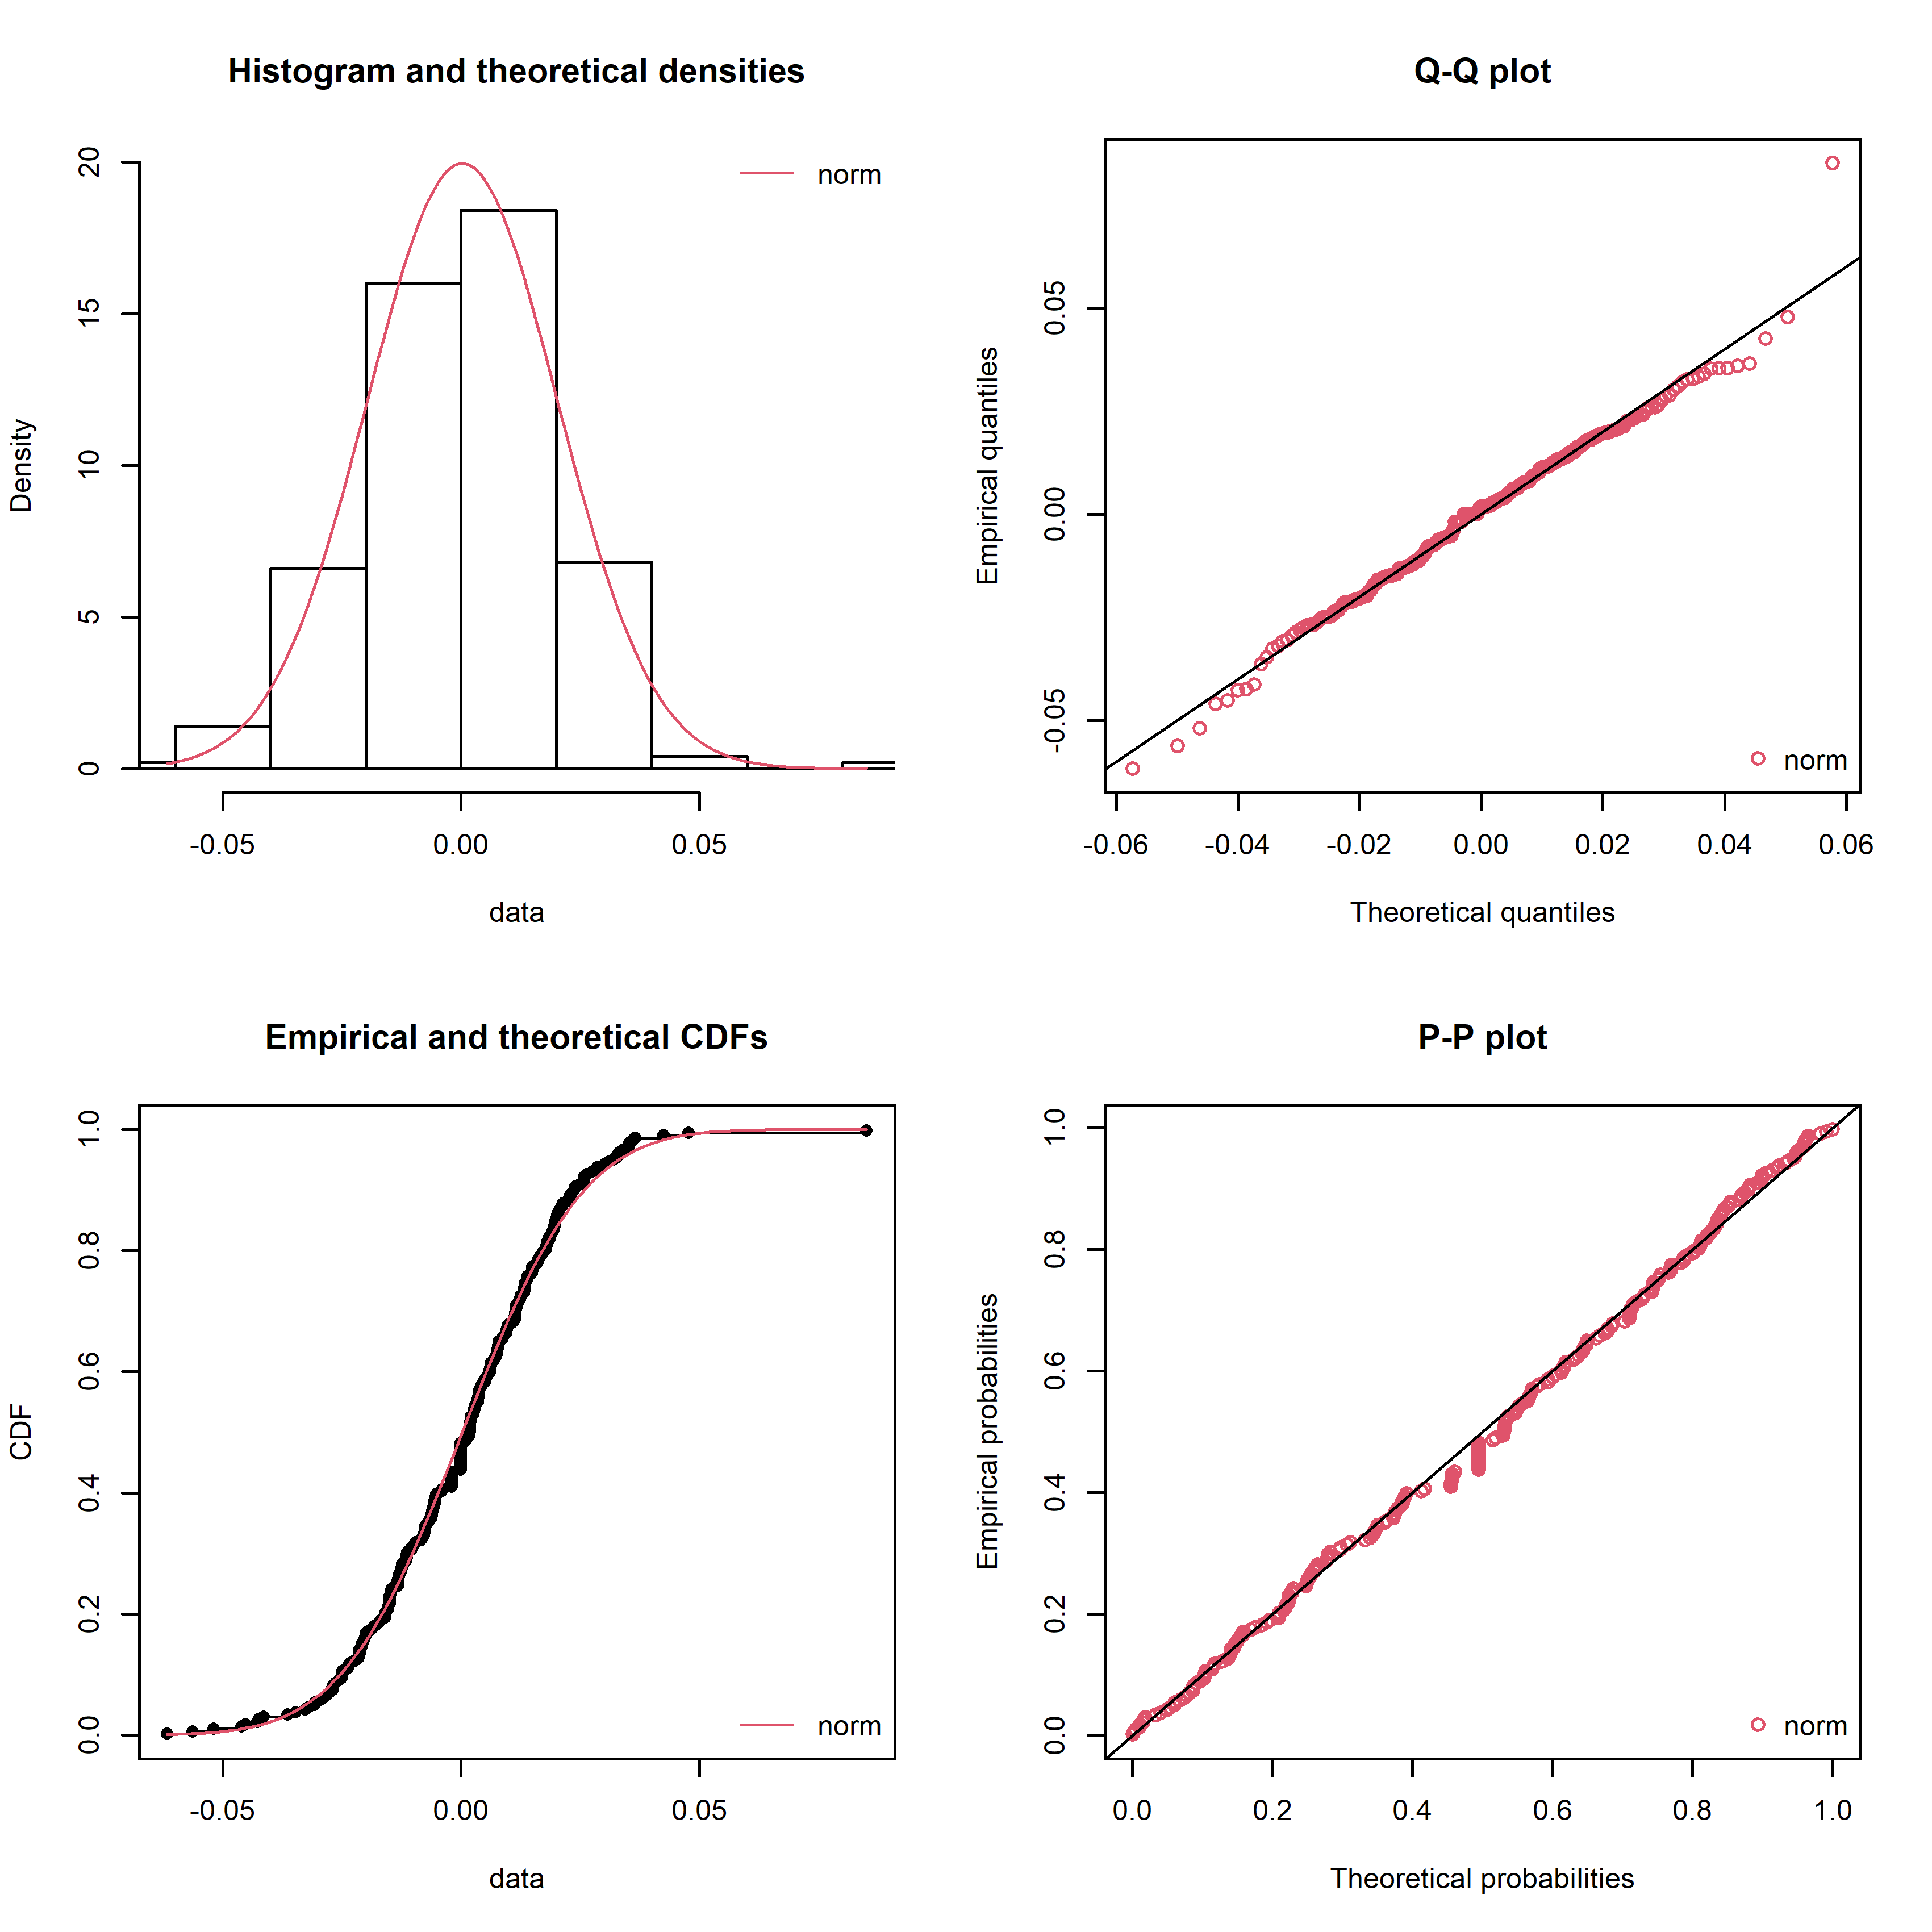
\includegraphics[width=10cm, height=10cm]{img/diff_11b_wykresy_diagnostyczne.png}
\caption{Wykres diagnostycznie log-zwrotów 11B}
\end{figure}

Wykresy diagnostyczne log-zwrotów spółki 11B wskazują, że rozkład normalny może pasować do opisywania log-zwrotów tej spółki

\newpage
\subsubsection{Test równości rozkładów metodą Monte Carlo dla spółki 11B}
W kontekście analizy log-zwrotów spółki 11 Bit Studios, przeprowadzony został test równości rozkładów z wykorzystaniem metody Monte Carlo. Poniżej zaprezentowany jest histogram z odległością dystrybuanty log-zwrotów oraz wyniki testu statystyki KS, który porównuje badany rozkład z rozkładem normalnym.

\begin{figure}[h]
\centering
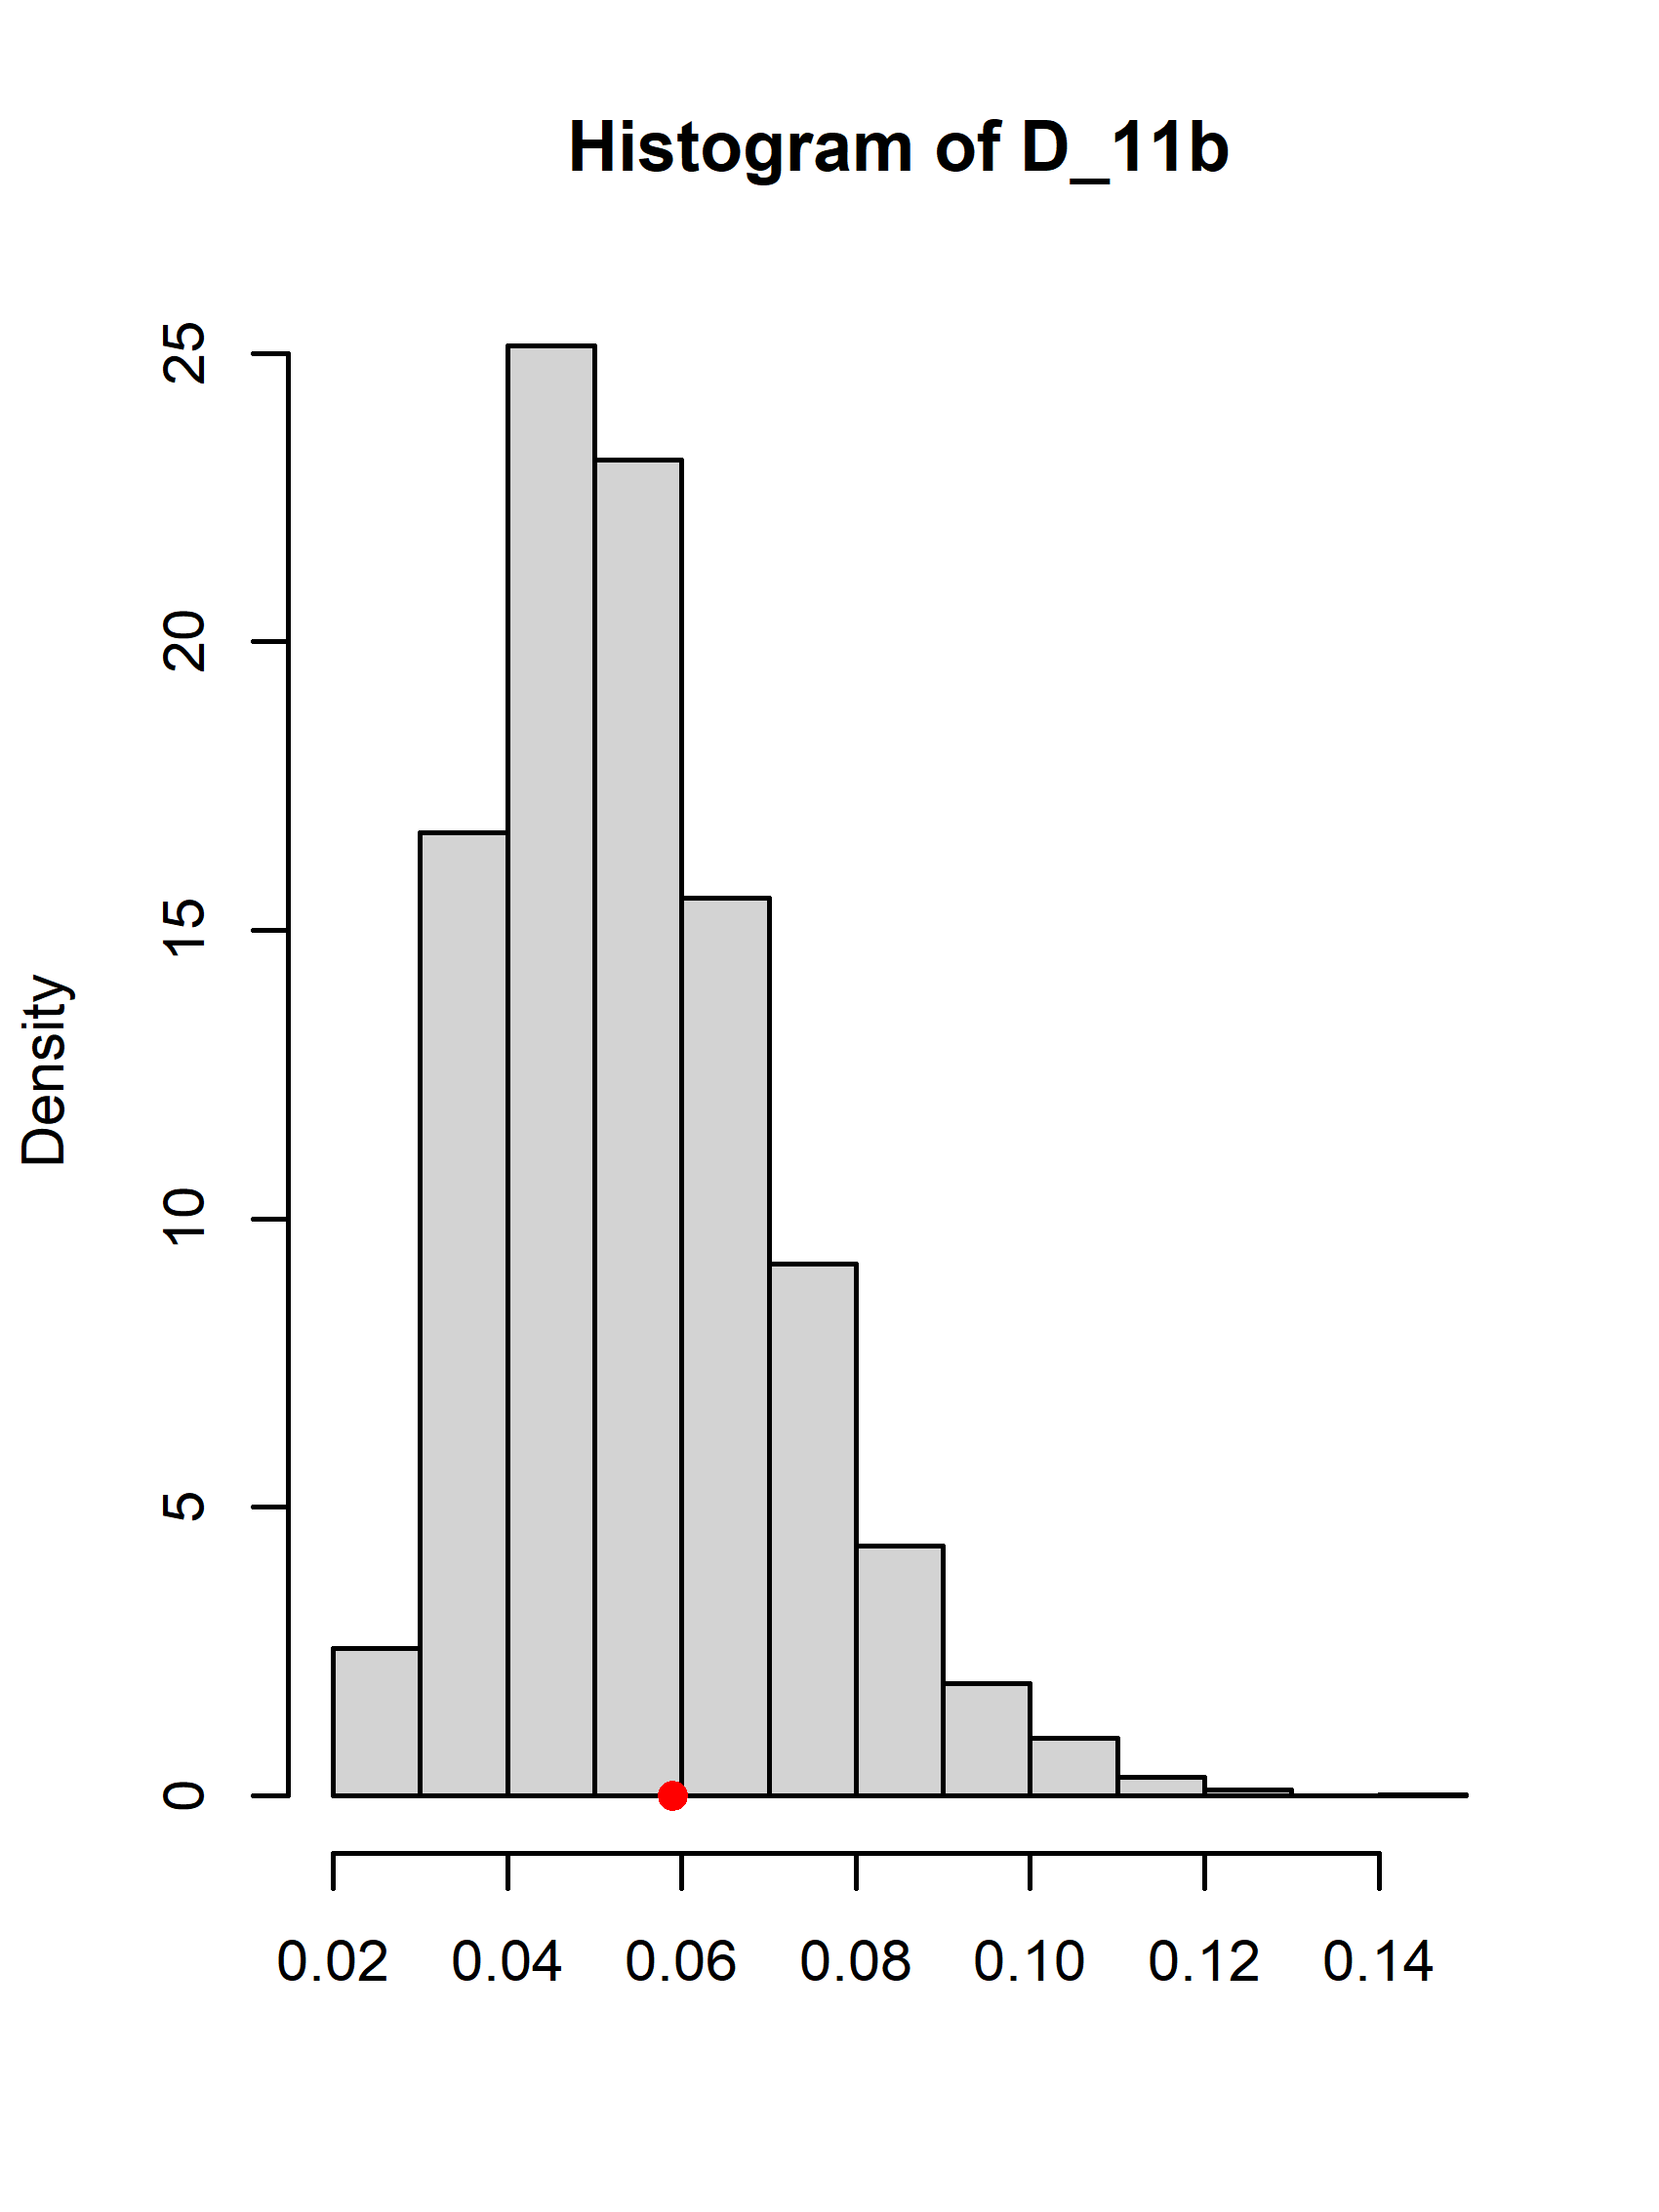
\includegraphics[width=9cm, height=12cm]{img/diff_11b_hipoteza_o_rownosci.png}
\caption{Histogram gęstości wyników testu KS próbek metody Monte-Carlo 11B}
\end{figure}

Testowałem rozkład normalny z wykorzystaniem statystyki KS. Wartość p-value wynosi 0.3376, a więc jest znacząco większa od przyjętego poziomu istotności (5\%), czyli nie ma podstaw do odrzucenia hipotezy zerowej, co oznacza, że możemy opisywać dane, czyli log-zwroty spółki 11B, za pomocą rozkładu normalnego

\newpage
\subsection{Estymacja parametrów rozkładu dwuwymiarowego normalnego oraz analiza
dobroci dopasowania}
W tej sekcji przeprowadzimy analizę rozkładu dwuwymiarowego normalnego, aby lepiej zrozumieć zależności między dwiema zmiennymi. Skoncentrujemy się również na analizie dobroci dopasowania, co pozwoli ocenić, jak dobrze model normalny pasuje do naszych danych.
\subsubsection{Wykres rozrzutu z histogramami rozkładów brzegowych}
W ramach analizy log-zwrotów spółek WMG.US i 11B, przepowadzona została estymacja parametrów rozkładu dwuwymiarowego normalnego. Poniżej przedstawiony jest wykres rozrzutu z histogramami rozkładów brzegowych, który pozwala na wizualną ocenę związku między log-zwrotami obu spółek w tym samym dniu handlowym.

\begin{figure}[h]
\centering
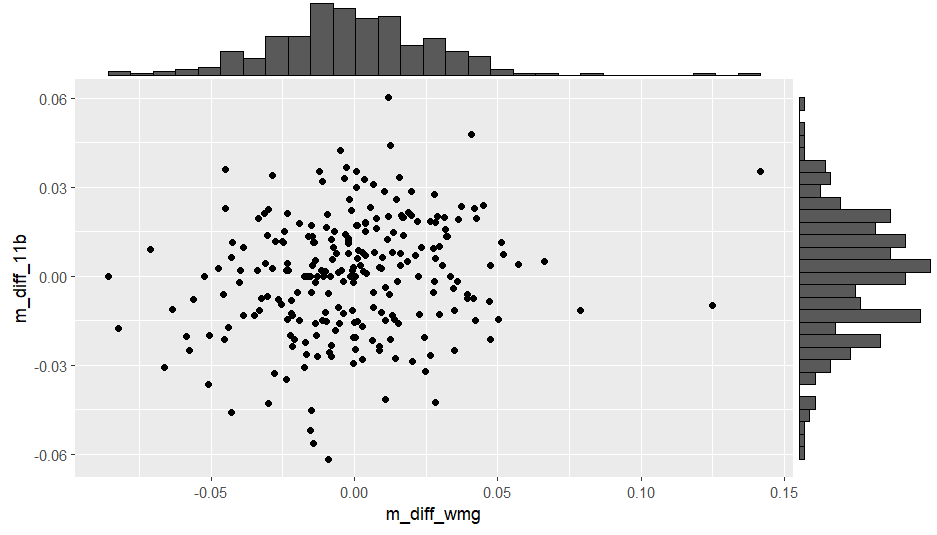
\includegraphics[width=12cm, height=12cm]{img/Rozrzut_z_histogramami.png}
\caption{Rozrzut z histogramami rozkładów brzegowych}
\end{figure}

Na Rysunku przedstawiono wykres rozrzutu z histogramami rozkładów brzegowych dla wspólnych dziennych(w tym samym dniu handlowym) log-zwrotów dla spółek WMG.US i 11B. Analiza wykresu wskazuje na brak wyraźnego związku między log-zwrotami wybranych spółek, co wskazuje na różne czynniki gospodarczo-rynkowe dla odmiennych branż, jakie reprezentują.

\newpage
\subsubsection{Wyznaczenie wektorów średnich \(\hat{\mu}\), kowariancji, współczynnik korelacji, macierz kowariancji \(\hat{\Sigma}\) oraz macierz korelacji}

\begin{itemize}
\item Wektor średnich:
\[
\hat{\mu} = \begin{pmatrix}
-0.0007550607 \\ % WMG.US
0.0002590858 % 11B
\end{pmatrix}
\]
Średnia dzienna dla WMG.US jest ujemna, a dla 11B co wskazuje odpowiednio, na spadek wartości akcji WMG.US i wzrost wartości dla 11B.

\item Macierz kowariancji(estymator nieobciążony):
\[
\hat{\Sigma} = \begin{pmatrix}
0.0008854081 & 0.0001087012 \\ % WMG.US
0.0001087012 & 0.0003969380 % 11B
\end{pmatrix}
\]
\item Macierz kowariancji(estymator obciążony):
\[
\hat{\Sigma} = \begin{pmatrix}
0.0008817645 & 0.0001082539 \\ % WMG.US
0.0001082539 & 0.0003953046 % 11B
\end{pmatrix}
\]

Wariancje na przekątnej macierzy wskazują na sporą zmienność dziennych log-zwrotów spółek. 

\item Macierz korelacji:
\[
P = \begin{pmatrix}
1.0000000 & 0.1833586 \\ % WMG.US
0.1833586 & 1.0000000 % 11B
\end{pmatrix}
\]
Współczynnik korelacji \(p = 0.1833\) opisje jak stopień zależności dwóch zmiennych. Jej wartość może wynosić od -1 do 1, co oznacza kolejno; całkowitą korelację ujemną i całkowitą korelację dodatnią. Im wspóczynnik jest bliższy zera tym mniej skorelowane są dane zmienne. Otrzyma wartość wskazuje na bardzo słabą zależność między log-zwrotami spółek WMG.US i 11B.
\end{itemize}

\subsubsection{Wzór gęstości rozkładu dwuwymiarowego o wysetymowanych parametrach \( N(\hat{\mu}, \hat{\Sigma}) \) oraz wzory gęstości rozkładów brzegowych}

\textbf{Wzór gęstości rozkładu dwuwymiarowego normalnego}
\smallskip

Wzór gęstości rozkładu dwuwymiarowego normalnego z wyestymowanymi parametrami \( \hat{\mu} \) i \( \hat{\Sigma} \). Funkcja gęstości jest określona wzorem:
\[
f(x, y) = \frac{1}{2\pi\sigma_X\sigma_Y\sqrt{1-\rho^2}} \exp\left(
-\frac{1}{2(1-\rho^2)}\left[
\frac{(x-\mu_X)^2}{\sigma_X^2} - 2\rho\frac{(x-\mu_X)(y-\mu_Y)}{\sigma_X\sigma_Y} + \frac{(y-\mu_Y)^2}{\sigma_Y^2}
\right]
\right),
\]
gdzie \( \mu_X = -0.0007550607 \), \( \mu_Y = 0.0002590858 \) są średnimi, \( \sigma_X = \sqrt{0.0008817645} \), \( \sigma_Y = \sqrt{0.0003953046} \) są odchyleniami standardowymi, a \( \rho = \frac{0.0001082539}{\sigma_X\sigma_Y} \) jest współczynnikiem korelacji pomiędzy zmiennymi \( X \) i \( Y \).

\subsubsection*{Wzory gęstości rozkładów brzegowych}

Rozkłady brzegowe dla zmiennych \( X \) i \( Y \) są rozkładami normalnymi z parametrami odpowiednio dla \( X \) i \( Y \). Wzory gęstości tych rozkładów są następujące:

Dla zmiennej \( X \):
\[
f_1(x) = \int_{-\infty}^{\infty} f(x, y) \, dy = \frac{1}{\sqrt{2\pi}\sigma_X^2} \exp\left(-\frac{(x-\mu_X)^2}{2\sigma_X^2}\right),
\]
gdzie \( \mu_X = -0.0007550607 \) i \( \sigma_X^2 = 0.0008817645 \).

Dla zmiennej \( Y \):
\[
f_2(y) = \int_{-\infty}^{\infty} f(x, y) \, dx = \frac{1}{\sqrt{2\pi}\sigma_Y^2} \exp\left(-\frac{(y-\mu_Y)^2}{2\sigma_Y^2}\right),
\]
gdzie \( \mu_Y = 0.0002590858 \) i \( \sigma_Y^2 = 0.0003953046 \).

\subsubsection*{Wykresy gęstości jednowymiarowych oraz wykres gęstości rozkładu
łącznego.}
Aby lepiej zrozumieć rozkłady log-zwrotów spółek 11B i WMG.US, analizujemy wykresy gęstości jednowymiarowych oraz wykres gęstości rozkładu łącznego.

\begin{figure}[h]
\centering
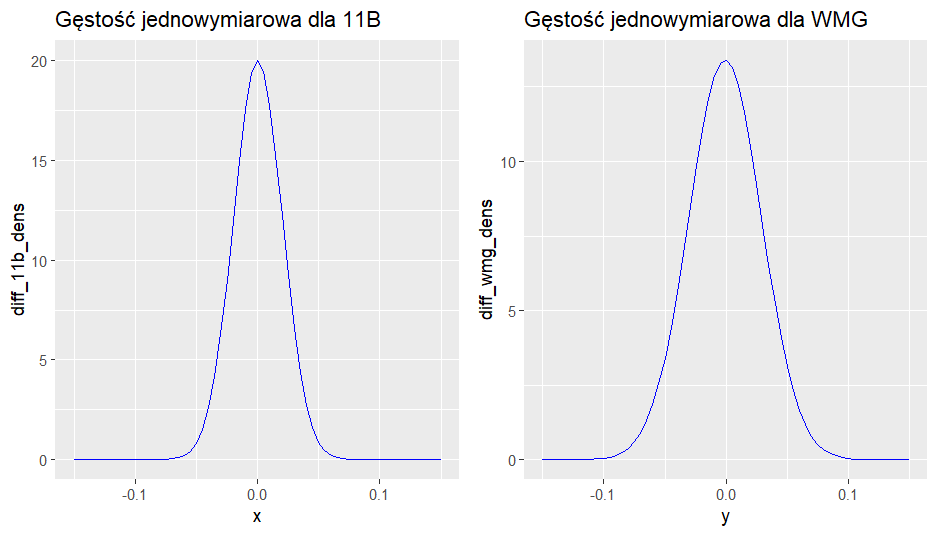
\includegraphics[width=16cm, height=5.333cm]{img/diff_wykresy_jednowymiarowe.png}
\caption{Wykresy jednowymiarowe spółek 11B i WMG.US}
\end{figure}


\begin{figure}[h]
\centering
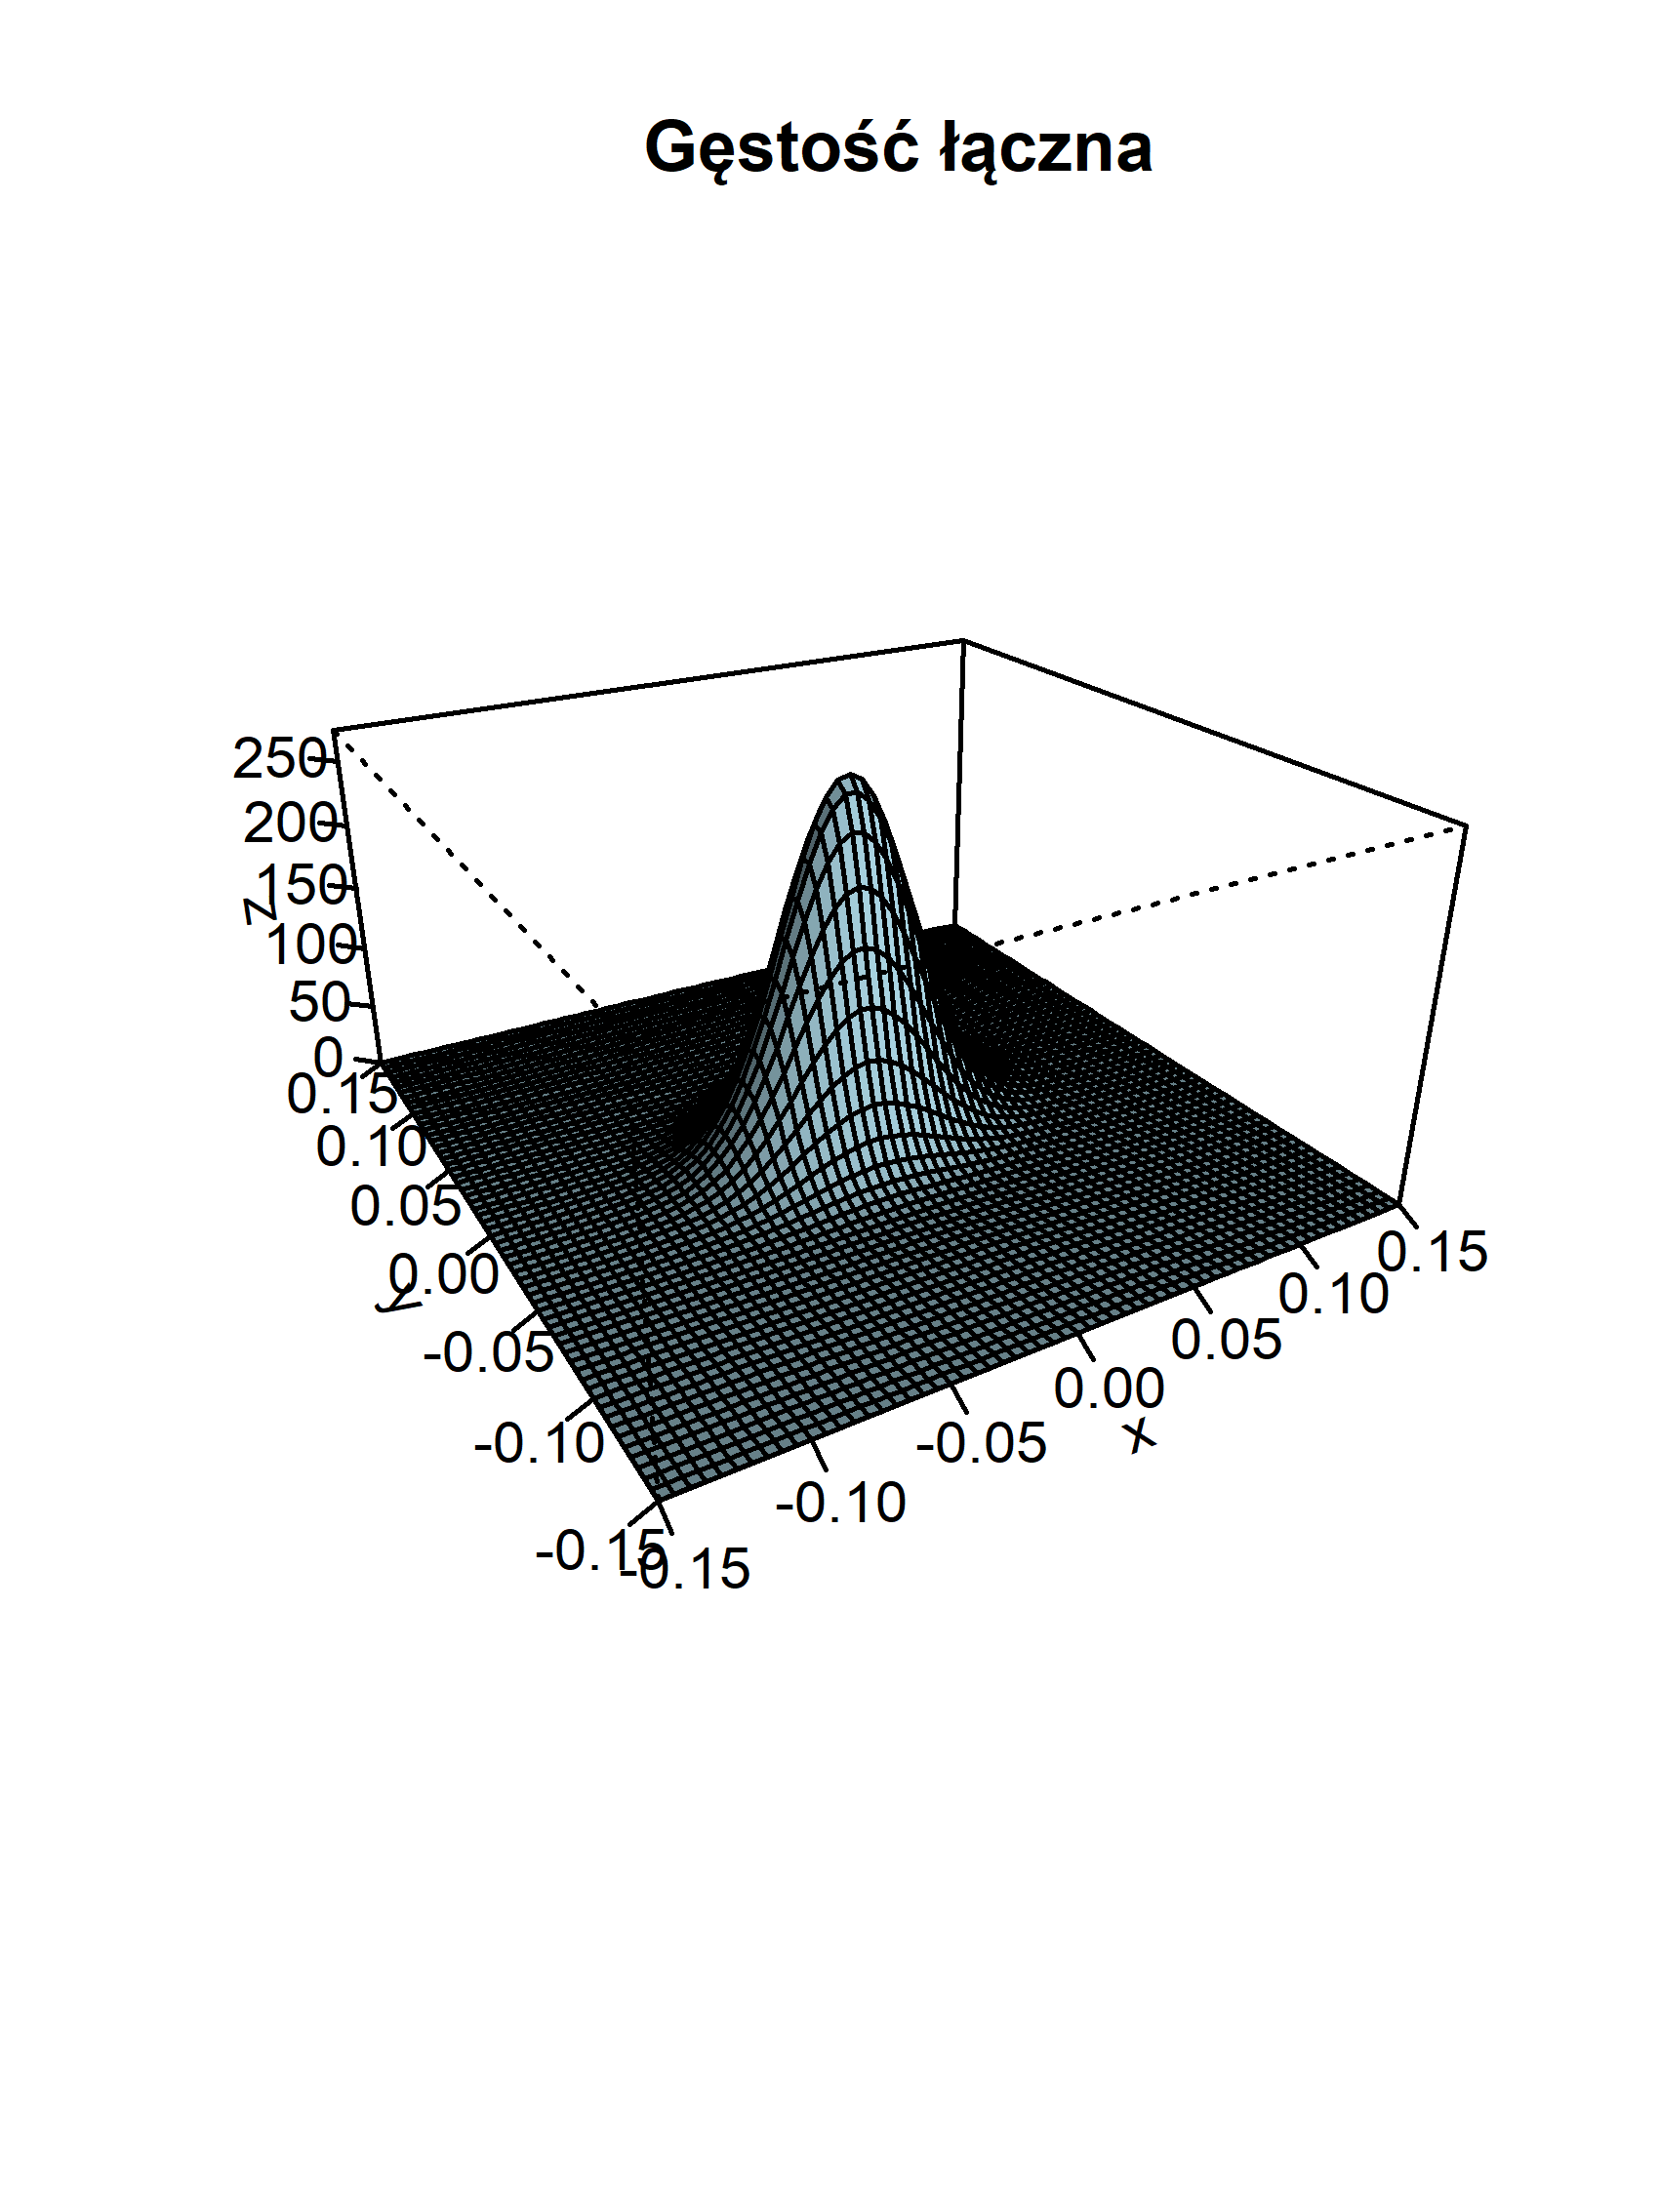
\includegraphics[width=12cm, height=12cm]{img/diff_gestosc_laczona_detailed.png}
\caption{Wykres gęstości rozkładu łącznego dla spółek WMG.US i 11B.}
\label{fig:densityPlot}
\end{figure}
\newpage

\subsection{Analiza dopasowania rozkładu normalnego, oznaczonego jako \( N(\hat{\mu}, \hat{\Sigma}) \)}

Dla otrzymanych za pomocą estymatorów parametrów \( \hat{\mu} \) i \( \hat{\Sigma} \) wylosowano próbę o takiej samej liczebności co rzeczywiste dane z rozkładu \( N(\hat{\mu}, \hat{\Sigma}) \)

\begin{figure}[h]
\centering
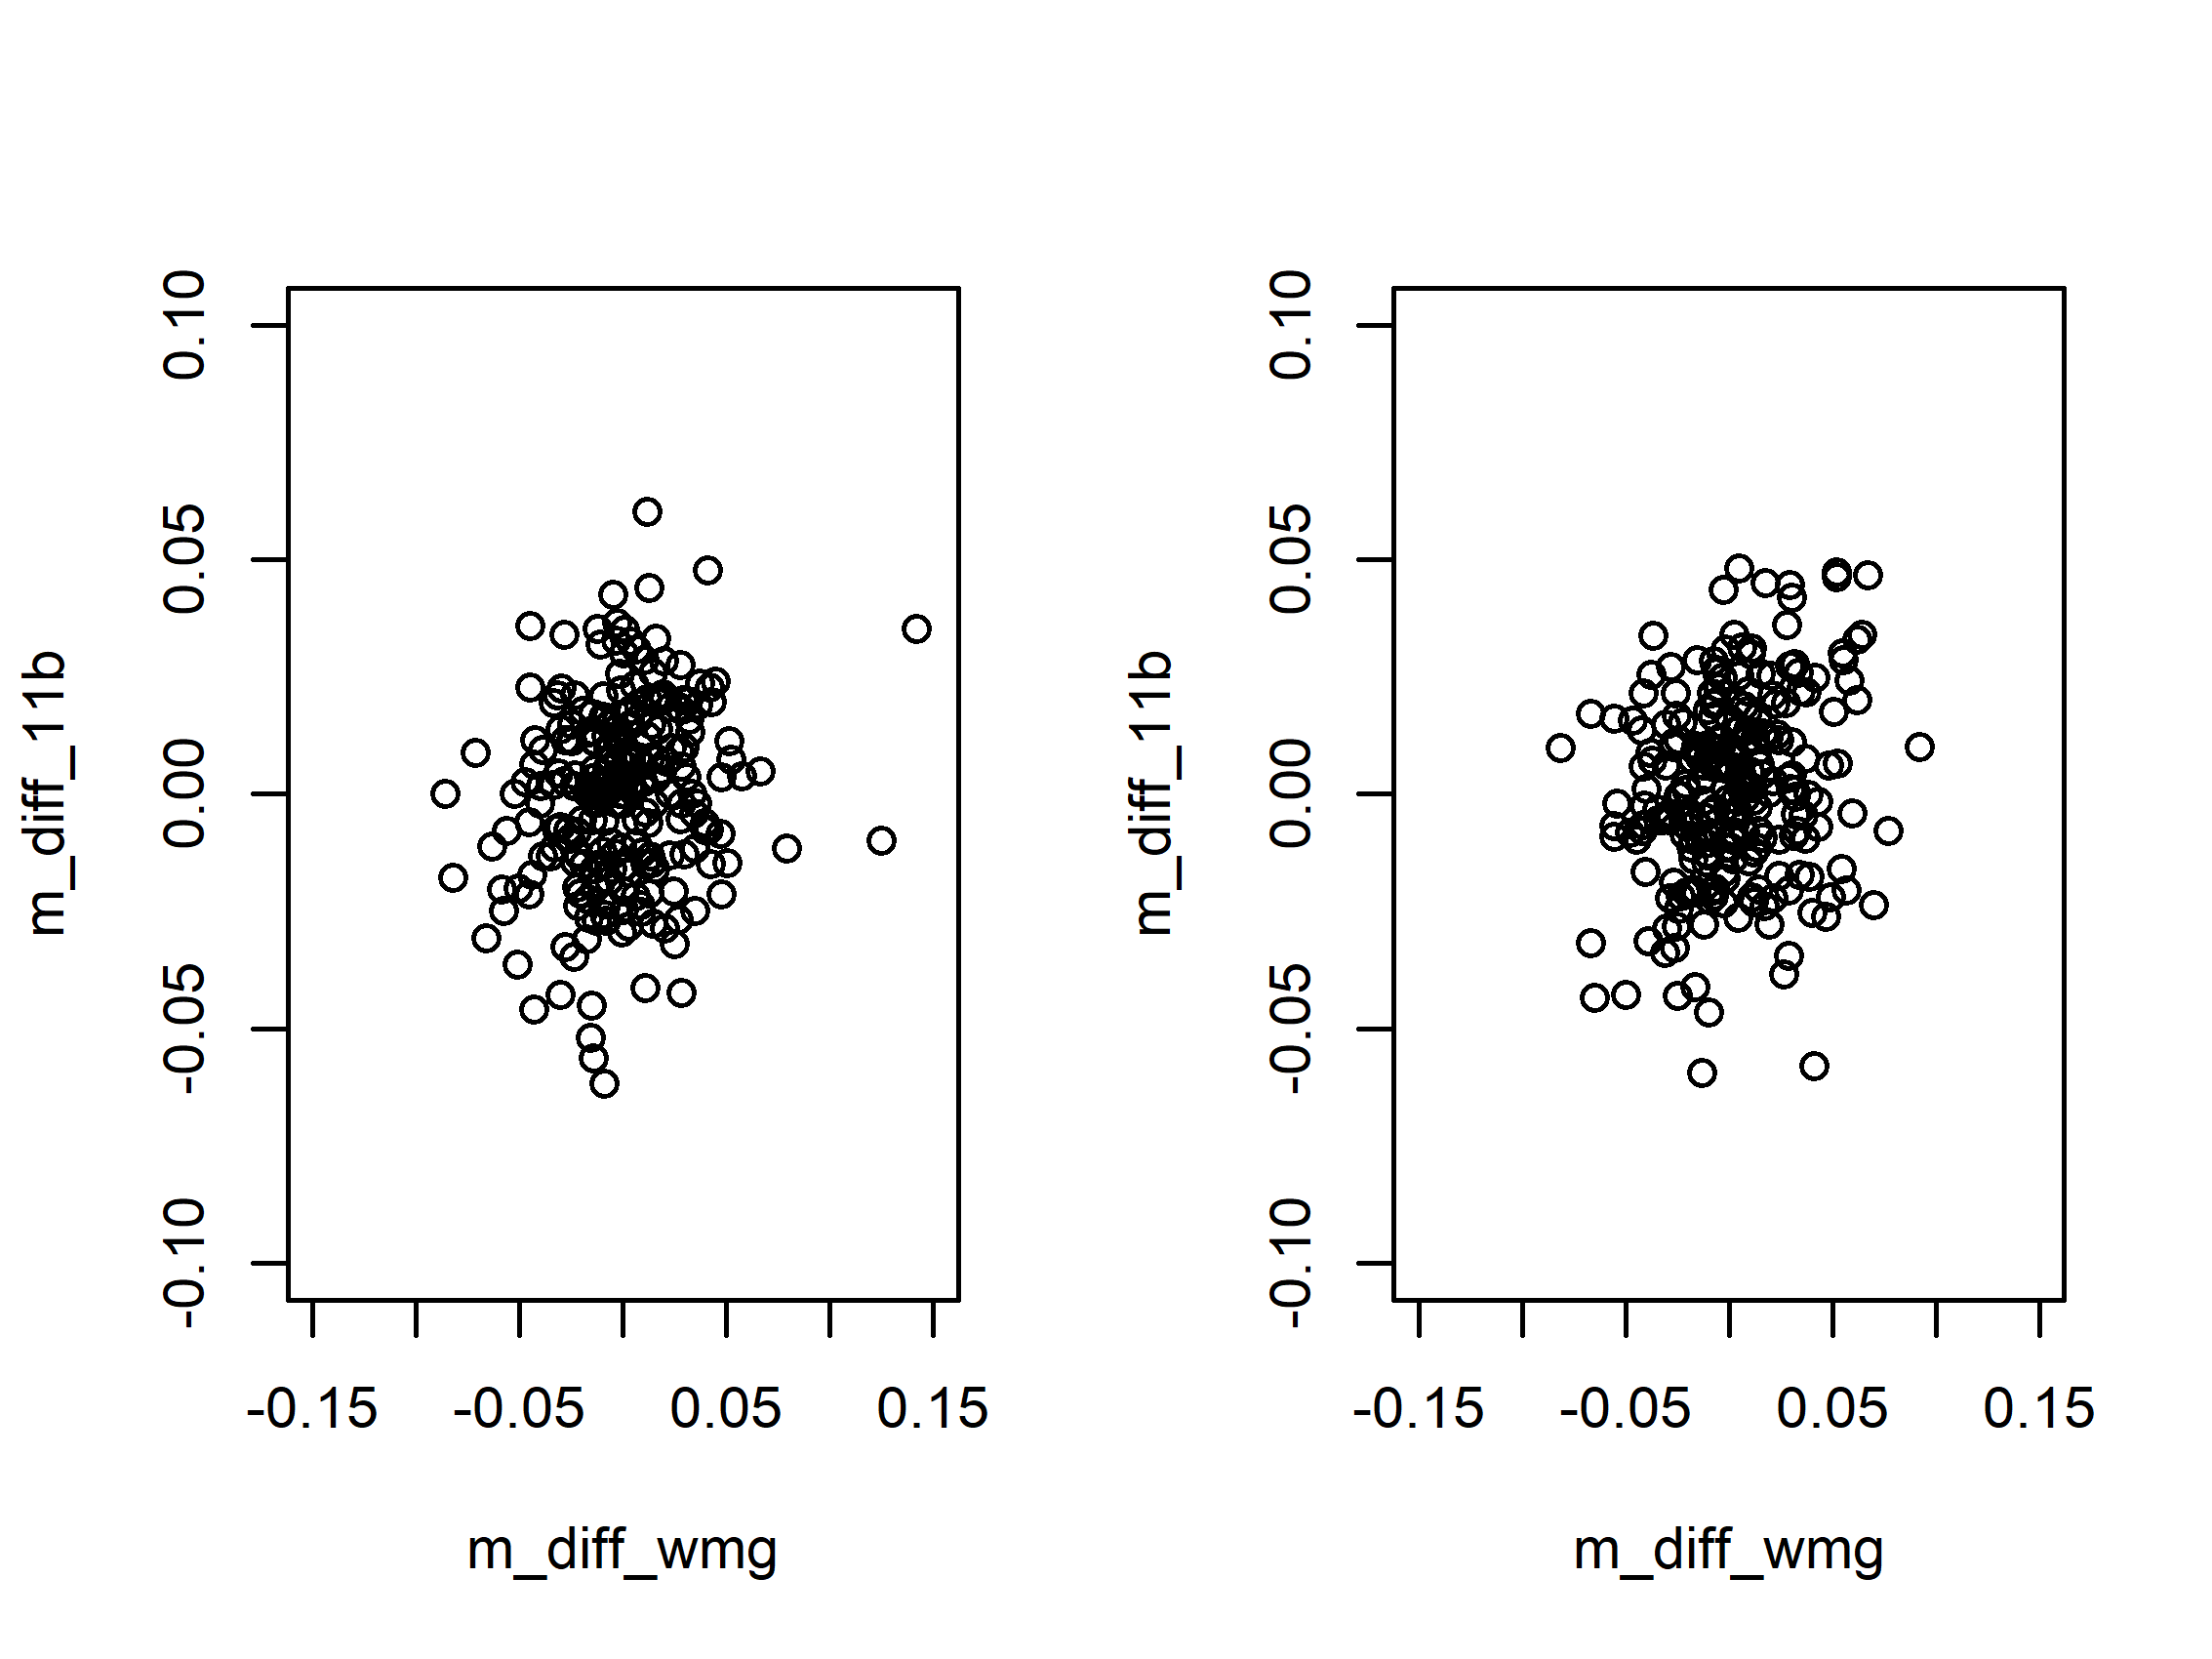
\includegraphics[width=12cm, height=9cm]{img/diff_wykresy_rozrzutu.png}
\caption{Wykresy rozrzutu dla otrzymanych danych(z lewej) i dla wygenerowanej próby(z prawej)}
\end{figure}

\smallskip

Porównując wykres otrzymany z danych do wykresu wygenerowanego z próby można stwierdzić, że model, stworzony z parametrów rozkładu bardzo dobrze oddaje rzeczywiste dane. Wyjątkiem są tylko dwa skrajne log-zwroty spółki WMG.US, co może wskazywać na mniejsze prawdopodobieństwo wydarzeń skrajnych dla stworzonego modelu. 


\begin{figure}[h]
\centering
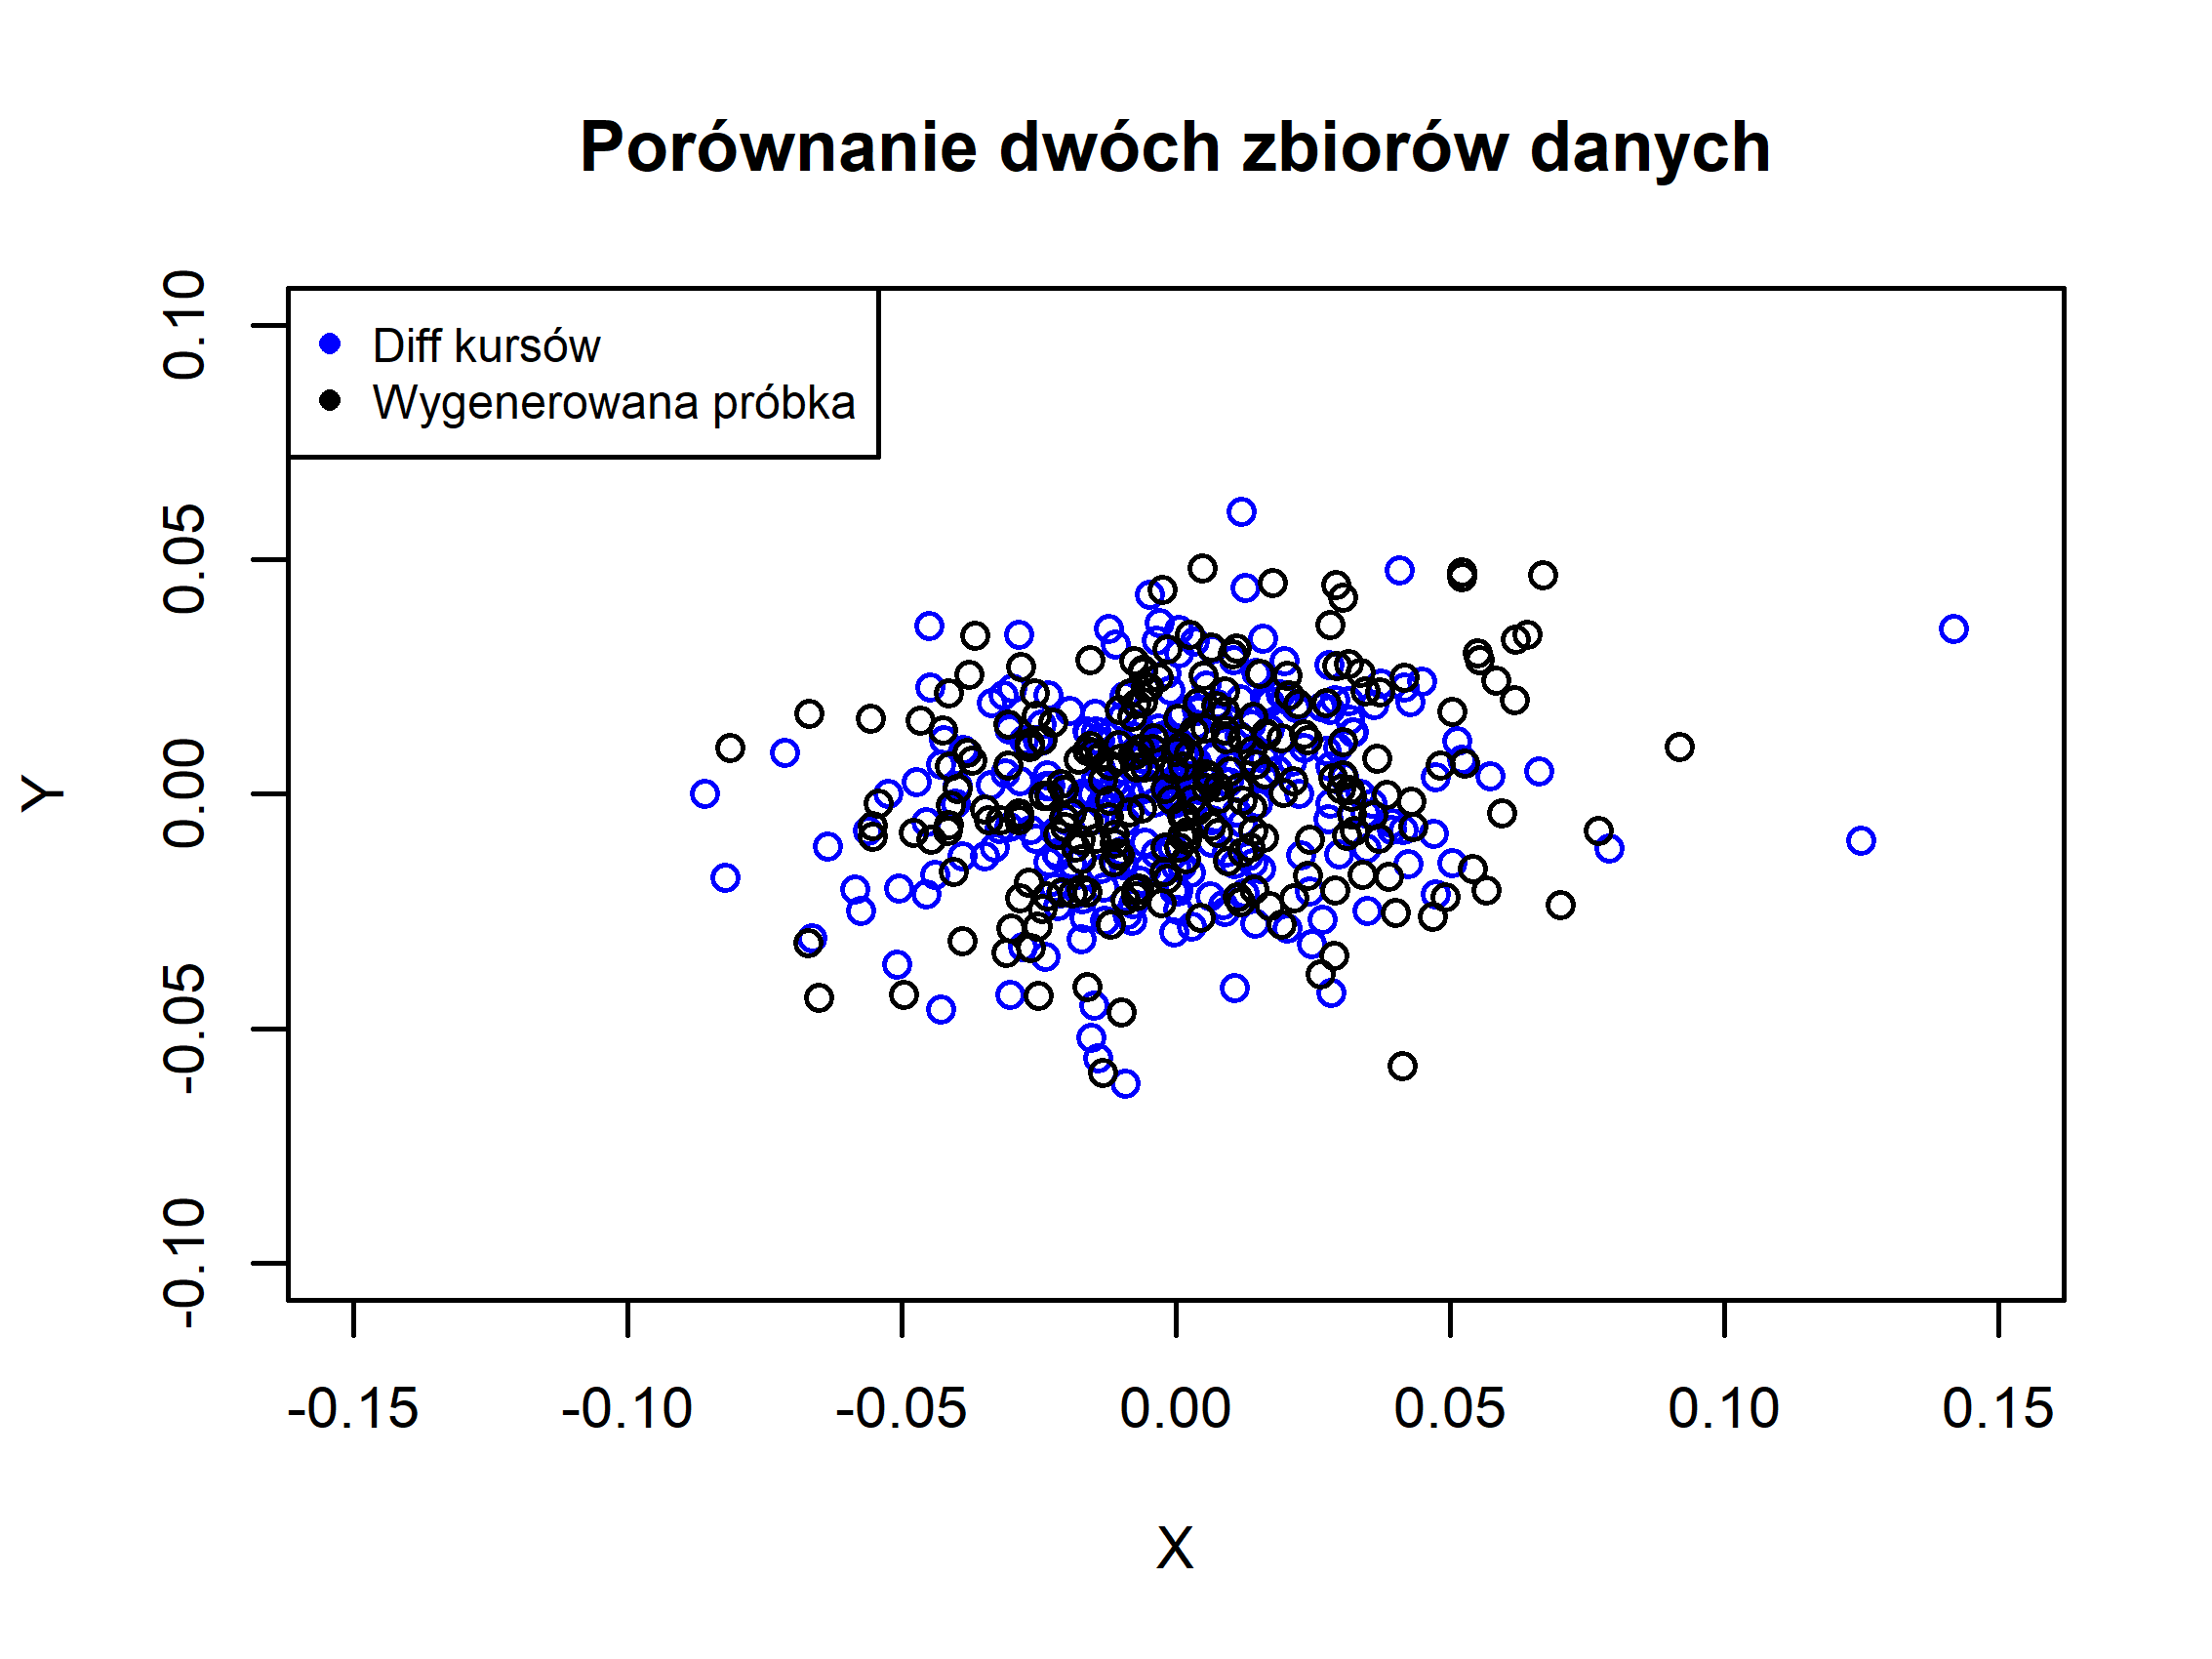
\includegraphics[width=10.66cm, height=8cm]{img/diff_porownanie_wykresow_rozrzutu.png}
\caption{Porównanie wykresów rozrzutu}
\end{figure}


\newpage
\section{Regresja liniowa}
W modelowaniu matematycznym regresja liniowa jest to metoda dopasowania linii lub krzywej (opisanej przez kombinację zmiennych i parametrów) reprezentującej oszacowaną wartość oczekiwaną zmiennej “y”, w naszym przypadku log-zwrotów spółki WMG.US przy konkretnych wartościach zmiennej “x” - odpowiednio log-zwrotów spółki 11B. Na wykresie podany układ “x” i “y” w połączeniu z naszymi danymi wygląda w następujący sposób:

\begin{figure}[h]
\centering
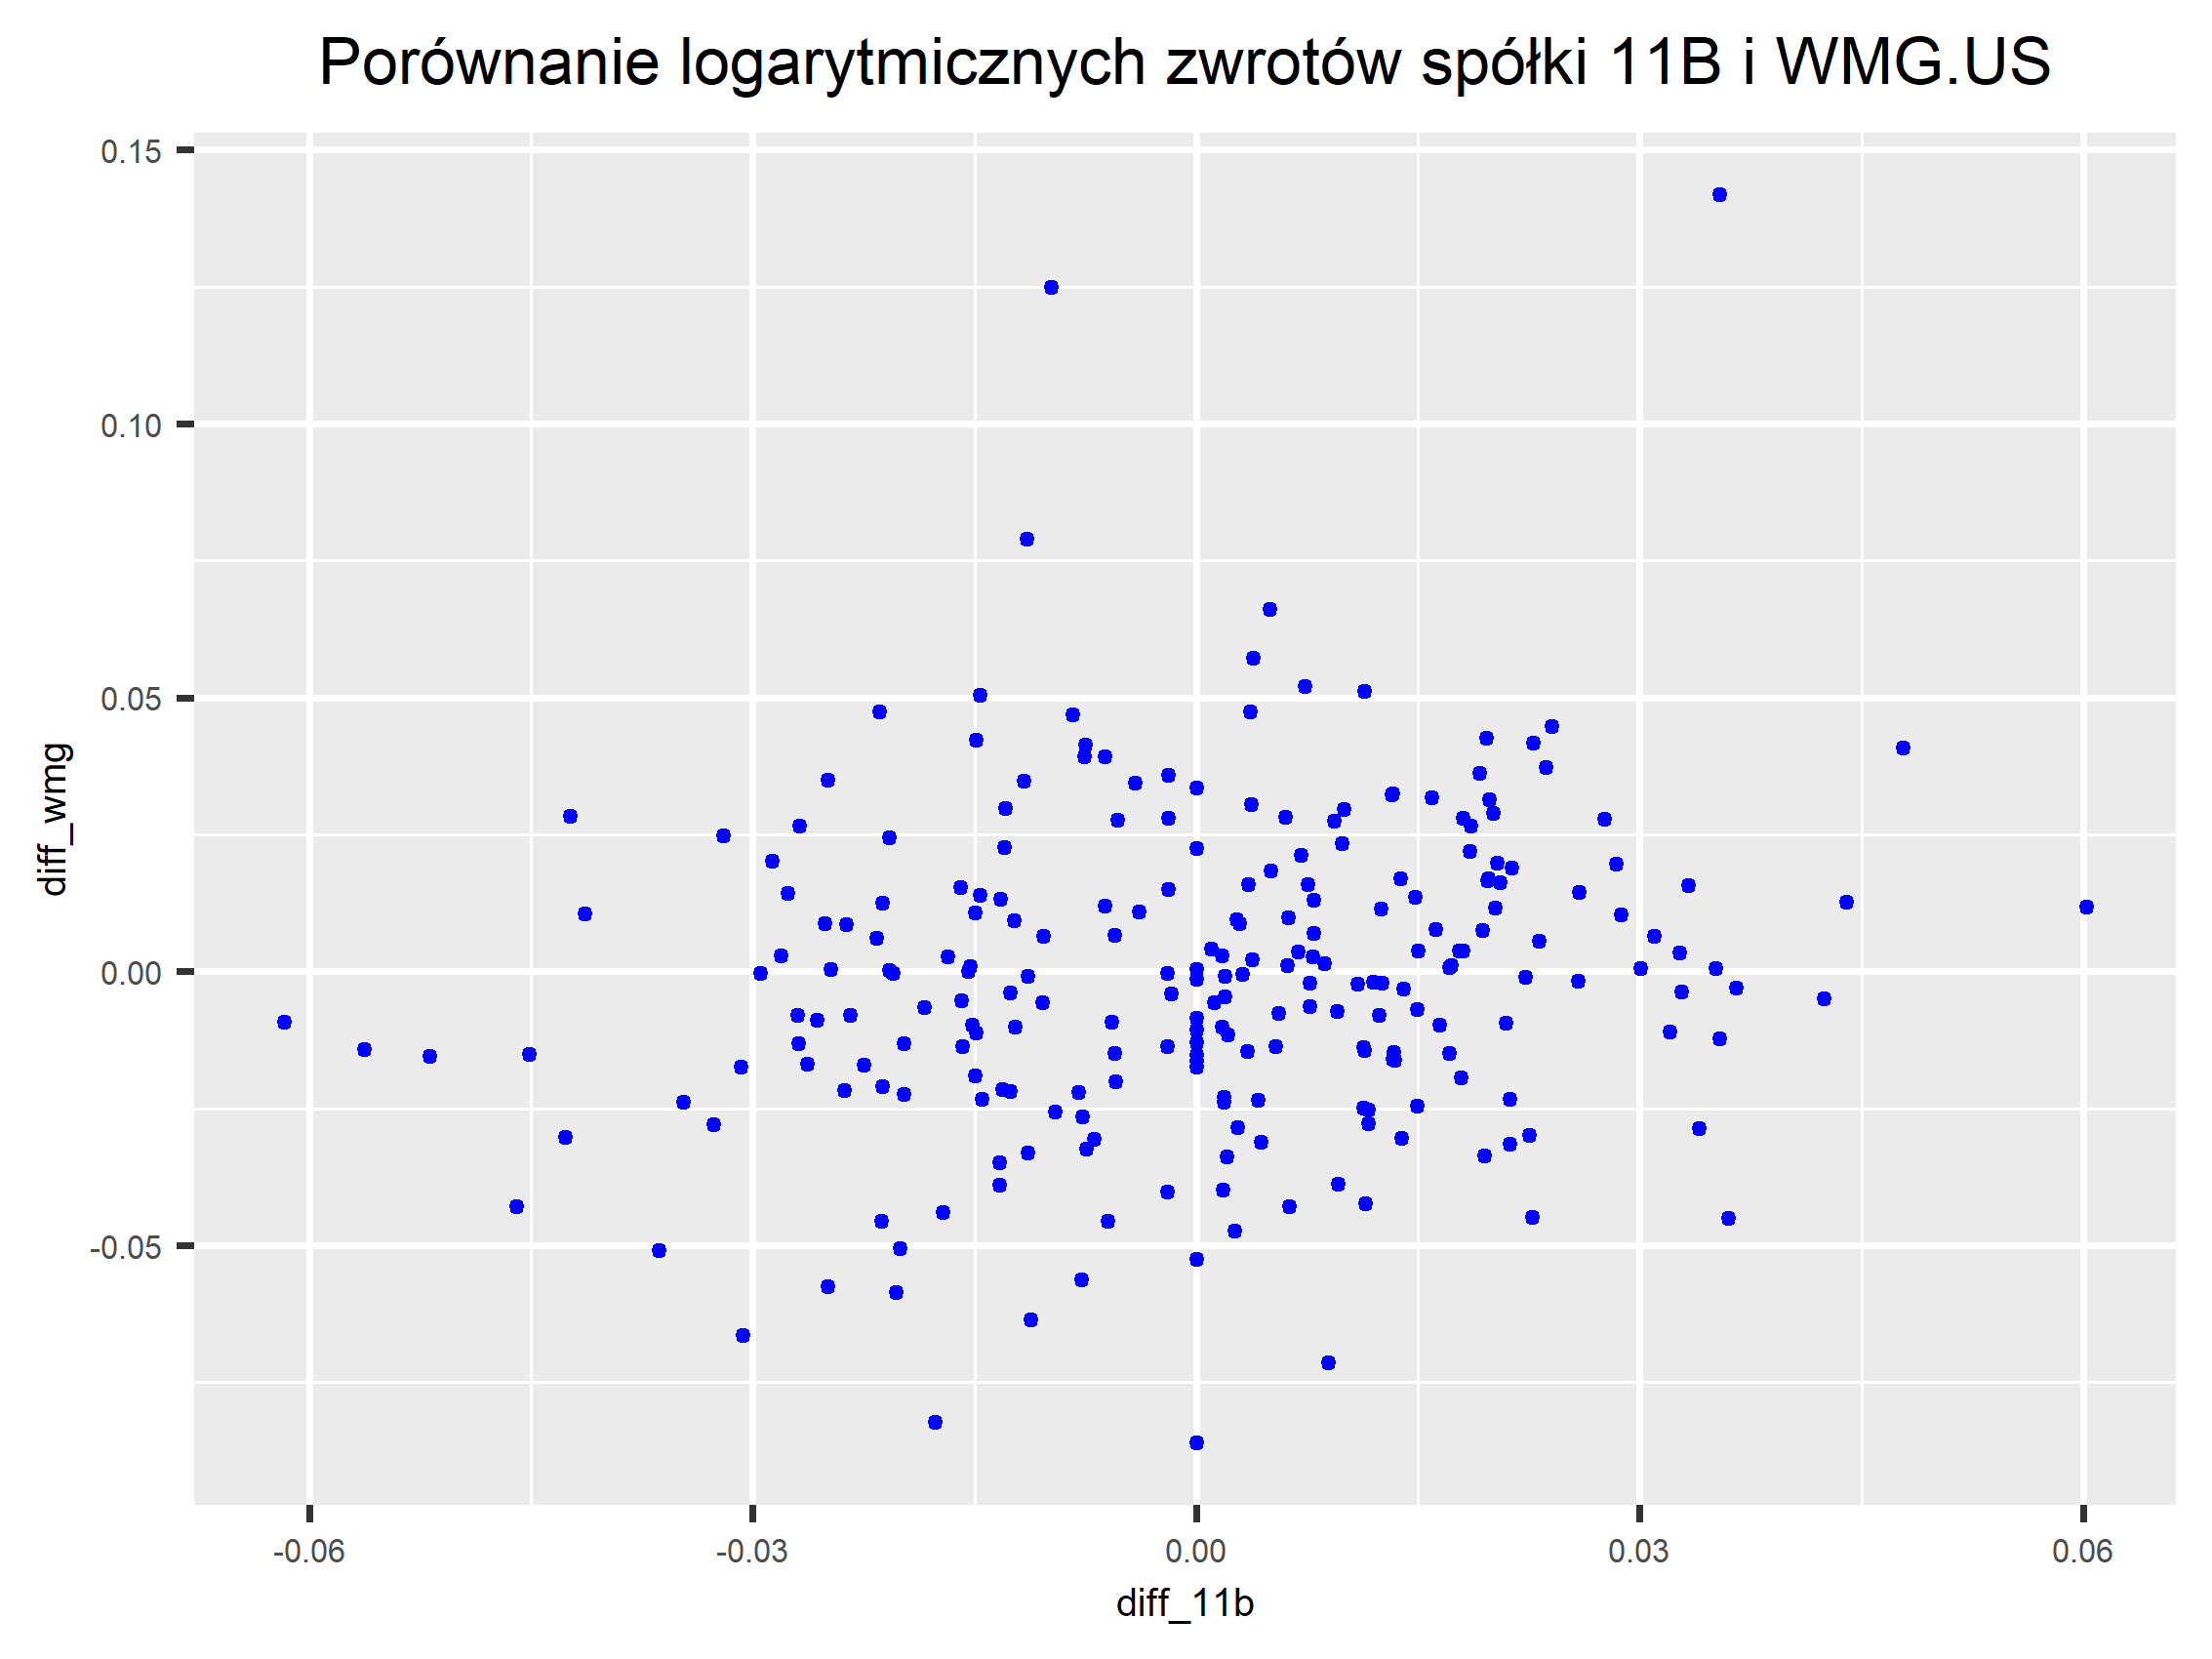
\includegraphics[width=12cm, height=9cm]{img/reg_porownanie.png}
\caption{Wykres porównania log-zwrotów spółek 11B i WMG.US}
\end{figure}

Z wykresu można zauważyć, że większośc danych oscyluje wokół \(y=0.00\), natomiast parametr “a” z funkcji liniowej \(y=ax+b\) będzie dodatni (funkcja rosnąca), ale nieduży (\(<\)1).


\subsection{Prosta regresji \(R_2 = b_0 + b_1 * R_1\)}
Do obliczenia parametrów \(b_0\) i \(b_1\) korzystamy z następujących wzorów:

\[
\beta_1 = \frac{\sum_{i=1}^{n} (x_i - \bar{x}_n)(y_i - \bar{y}_n)}{\sum_{i=1}^{n} (x_i - \bar{x}_n)^2}
\]
\[
\beta_0 = y_n - x_n \beta_1,
\]
\[
\quad \text{gdzie} \quad x_n = \frac{1}{n} \sum_{i=1}^{n} x_i, \quad y_n = \frac{1}{n} \sum_{i=1}^{n} y_i.
\]

Podstawiając uzyskane dane otrzymujemy następujące parametry:

\[b_1 = 0.2738 \text{, }b_0 = -0.0008\]

A zatem prosta regresji określona będzie wzorem:

\[y = 0.2738 * x - 0.0008\]

\newpage

Na wykresie wyestymowany model regresji przestawia się następująco

\begin{figure}[h]
\centering
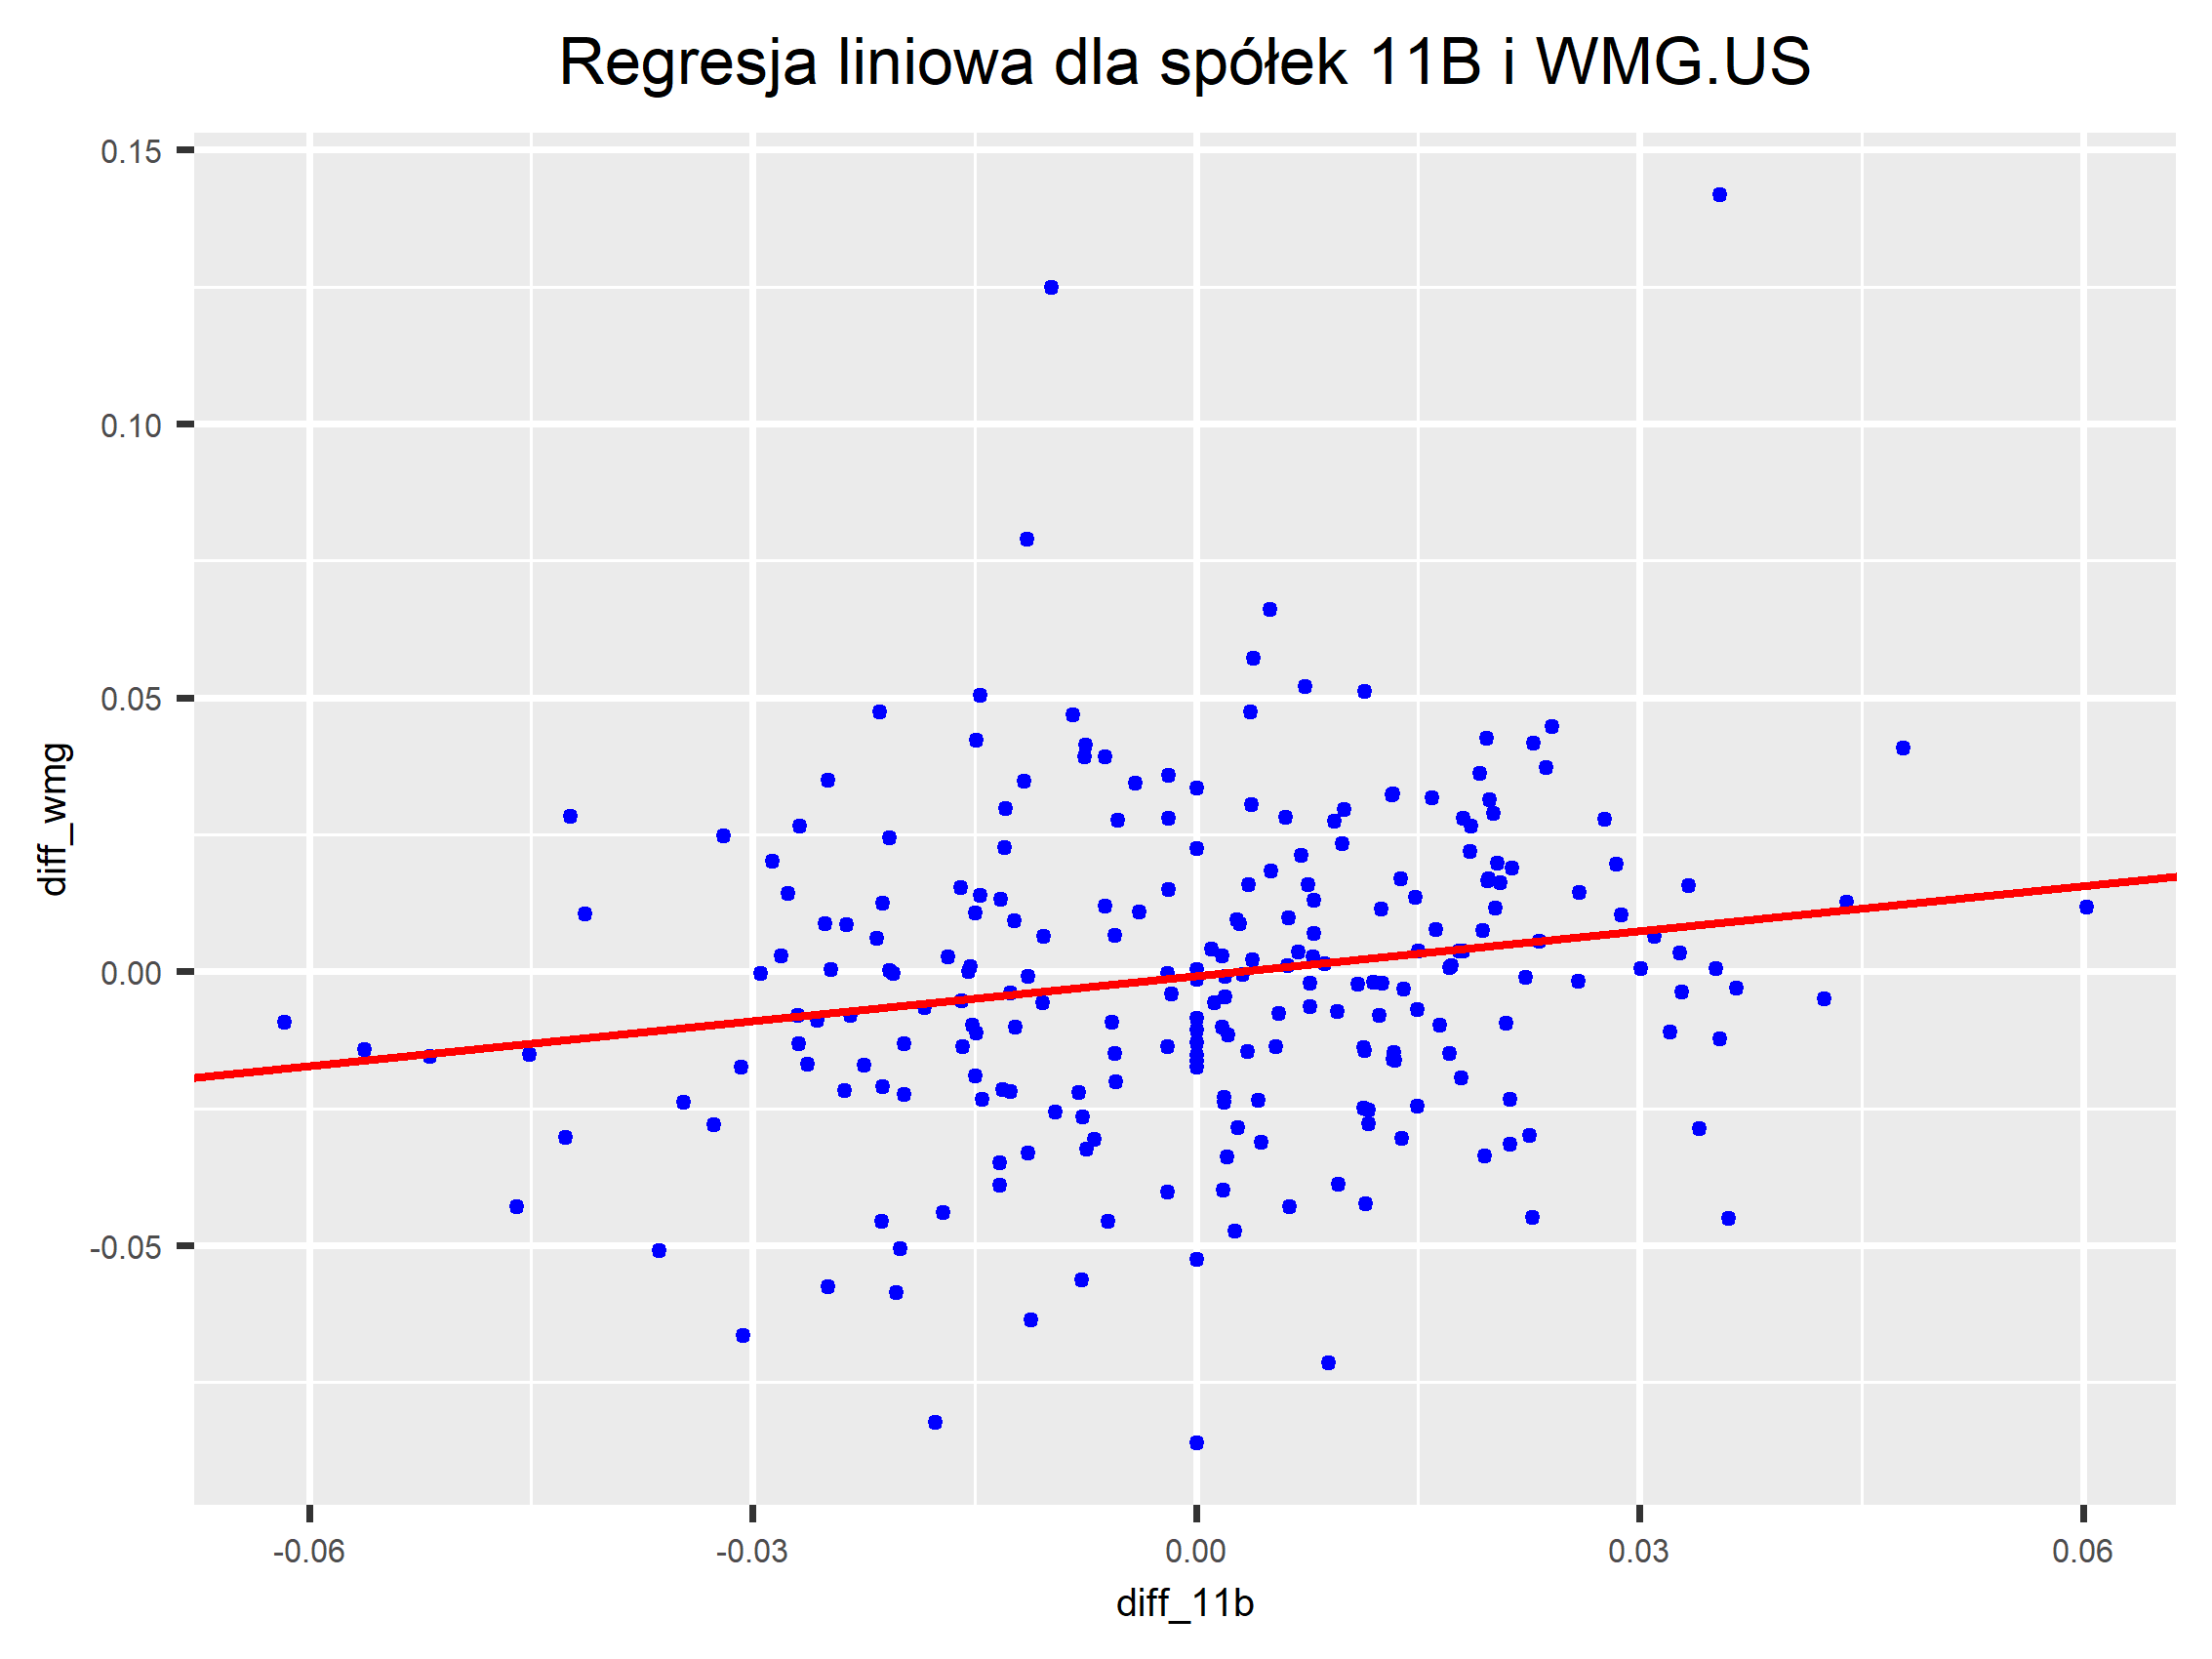
\includegraphics[width=12cm, height=9cm]{img/reg_regresja.png}
\caption{Wykres log-zwrotów 11B i WMG.US z prostą, przedstawiającą regresję liniową tych spółek}
\end{figure}


\subsection{Reszty modelu \(\epsilon \sim \mathcal{N}(0, \sigma^2)\).}

Każdy model liniowy jest obarczony pewnym błędem. Aby go określić stwórzmy model błędu reszt (\(\epsilon\)), czyli różnic między modelem liniowym, a otrzymanymi danymi, zapisaną jako rozkład normalny o parametrach (0, \(\sigma^2\)), a następnie przetestujmy hipotezę o normalności rozkładu błędu. 

Nieobciążony estymator wariancji błędów jest sumą kwadratów reszt, podzieloną przez liczność próby pomniejszoną o dwa:
\[\hat{\sigma}^2 = \frac{1}{n-2} \sum_{i=1}^{n} \epsilon_i^2
\]

Po spierwiastkowaniu otrzymujemy \(\sigma\), którą nazywamy Błędem standardowym reszt (RSE - Residual Standard Error):
\[RSE = \hat{\sigma} = \sqrt{\frac{\sum_{i=1}^{n} \epsilon_i^2}{n-2}}
\]

Po podstawieniu danych, otrzymujemy:
\[RSE = \sigma = 0.029\]


\begin{figure}[h]
\begin{minipage}{0.4\textwidth}
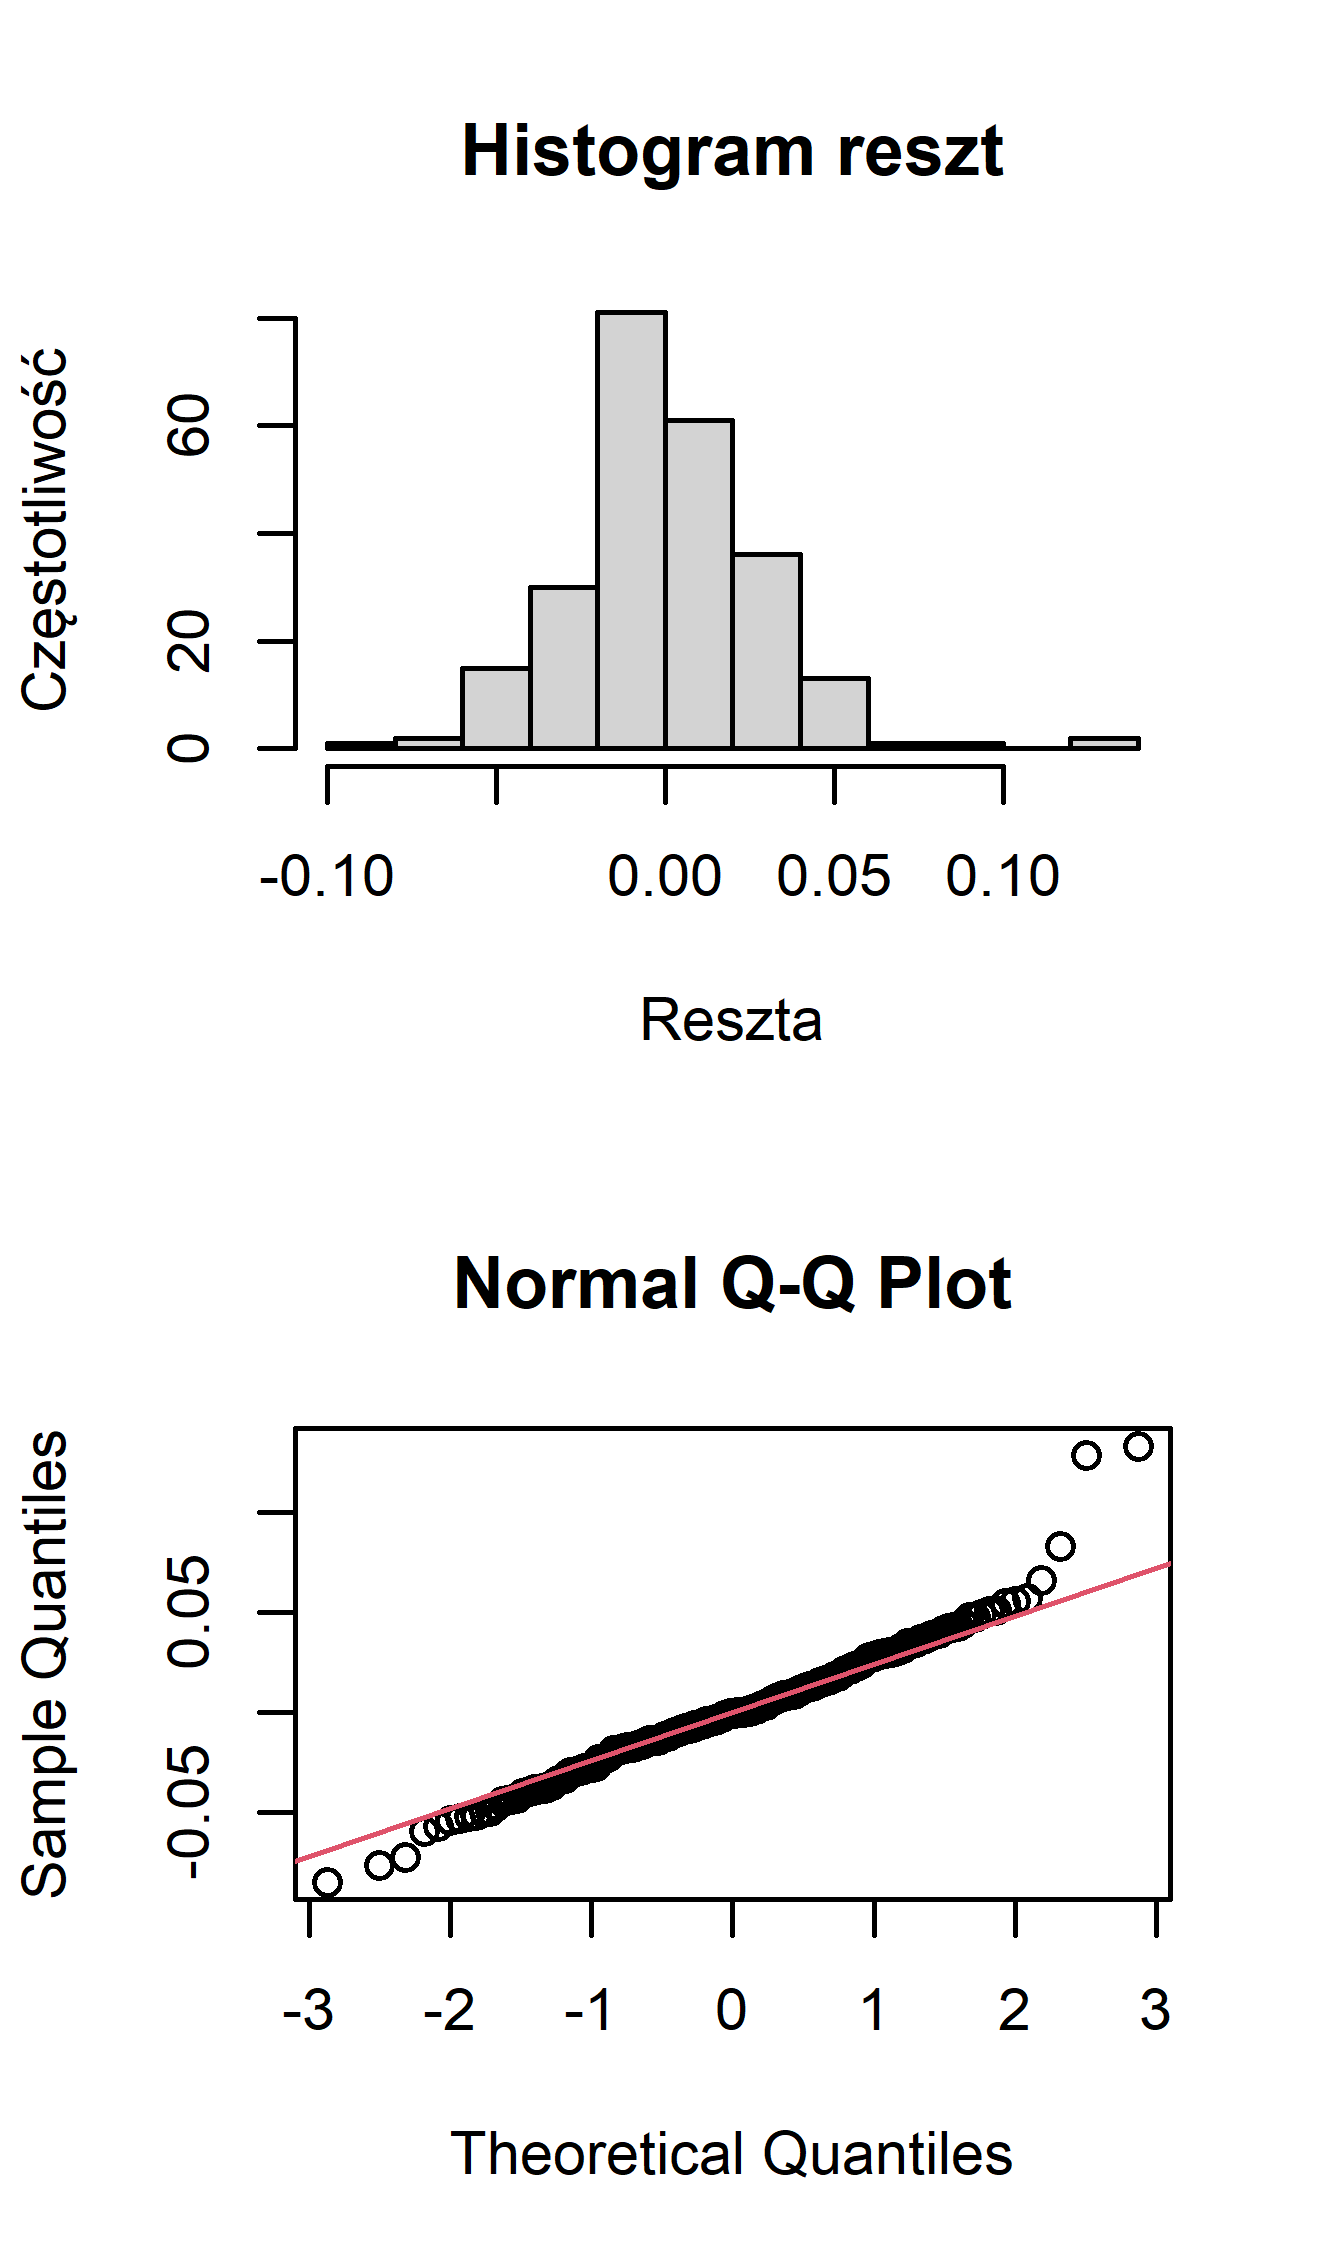
\includegraphics[height=14cm]{img/reg_hist_i_qq_ver.png}
\end{minipage}
\hfill
\begin{minipage}{0.5\textwidth}
\hspace*{0.4cm}Po określeniu parametrów rozkładu testujemy hipotezę o normalności rozkładu błędu, gdzie \(H_0\) - rozkład błędu jest normalny, przeciwko \(H_1\) - rozkład błędu nie jest opisany rozkładem normalnym.

\hspace*{0.4cm}Do testów skorzystamy ze statystyk KS i AD, które są opisane w poprzednim rozdziale.

\hspace*{0.4cm}Dla \textbf{KS p-value wyniosło \(p=0.3488\)}, a \textbf{dla AD \(p=0.0098\)}.

\hspace*{0.4cm}Zatem na poziomie istotności 5\% dla statystyki KS nie ma podstaw do odrzucenia hipotezy zerowej, natomiast dla statystyki AD odrzucamy hipotezę zerową. Biorąc pod uwagę, że statystyka KS jest mniej znacząca niż AD (test AD ma lepsze właściwości, na przykład zwraca większą uwagę na wartości skrajne), można dojść do wniosku, że rozkład błędu nie jest opisany rozkładem normalnym. Gdybyśmy jednak nie mieli podstaw do odrzucenia hipotezy zerowej, model regresji dla uzyskanych danych wyglądałby następująco:
\[y = 0.2738 * x - 0.0008 + \epsilon, \epsilon \sim \mathcal{N}(0, 0.029^2 )\]


\end{minipage}
\end{figure}

\newpage
\subsection{Współczynnik determinacji}

Kolejną miarą jakości dopasowania modelu regresji liniowej do danych jest współczynnik determinacji \(R^2\). Informuje ona, jaka część danych pokrywa się ze zmiennymi zawartymi w modelu (czyli jaką część danych wyjaśnia nasz model). Przyjmuje ona wartości z przedziału \([0;1]\), wyrażana jest najczęściej w procentach i im bliższa jest jedynki, tym dopasowanie modelu jest lepsze.

Współczynnik determinacji \(R^2\) określamy wzorem:
\[R^2 = 1 - \frac{\sum_{i=1}^{n} \epsilon^2}{\sum_{i=1}^{n} (y_i - \bar{y})^2}\]

Dla przedstawionych danych otrzymano: 
\[R\approx0.034\approx3,4\%\]



W utworzonym modelu regresji dla log-zwrotów spółek 11B i WMG.US (\(y = 0.2738 * x - 0.0008 + \epsilon, \epsilon \sim \mathcal{N}(0, 0.029^2 )\)), współczynnik determinacji \(R\approx3,4\). Czyli prawie 97\% log-zwrotów spółki WMG.US nie jest wyjaśniona przez 11B, a co za tym idzie należałoby dołączyć do stworzonego modelu dodatkowe zmienne.

\newpage
\subsection{Analiza istotności współczynników regresji \(b_0\) i \(b_1\)}
Kolejnym krokiem w tworzeniu modelu regresji liniowej jest określenie istotności współczynników \(b_0\) i \(b_1\). W przypadku gdy któryś ze wspóczynników okaże się nieistotny, zostatnie utworzony model uproszczony bez niego.

\subsubsection{Współczynnik \(b_1\)}

Istnieją hipotezy:
\(H_0\): \(b_1=0\) przeciwko \(H_1\): \(b_1\neq0\),

\[T = \frac{b_i - \beta_i}{\text{se}(\beta_i)}, \quad 
\] \(\text{gdzie} \quad \text{se}(\beta_i)\) to błąd standardowy estymatora (RSE).

\textbf{Dla podanego współczynnika \(i=1\) w podanym wzorze}

Sama statystyka \(T\) ma rozkład  \textit{t}-Studenta o \(n-2\) stopniach swobody. W analizowanych danych \(n=244\), a więc jeśli hipoteza \(H_0\) jest prawdziwa, to statystyka T ma rozkład t-Studenta o 242 stopniach swobody. Zarówno skrajnie duże, jak i skrajnie małe wartości statystyki świadczą przeciwko hipotezie zerowej.



Hipotezę zerową \(H_0\) odrzucamy, gdy wartość statystyki \(T\), obliczona dla danych jest “zbyt daleko od centrum rozkładu” \textit{t}-Studenta. Aby to określić korzystamy z wartości nazwanej jako \textit{p}-value którą obliczamy ze wzoru 
\[p-value = P(T > |t-value|),\]

gdzie \textit{t}-value to estymator współczynnika \(b_1\) dzielony przez błąd standardowy.
Wartość statystyki testowej obliczona dla danych wynosi kolejno:
\[t-value = 2.896 \text{, }p-value = 0.004\]

Z obliczeń wynika, że \textit{p}-value jest mniejsze od poziomu istotności wynoszącego 5\%, więc istnieją podstawy do odrzucenia hipotezy zerowej, a więc współczynnik \(b_1\) nie może być równy 0 w stworzonym modelu.

\subsubsection{Współczynnik \(b_0\)}

Istnieją hipotezy:
 \(H_0\): \(b_0=0\) przeciwko \(H_1\): \(b_0\neq0\), gdzie statystyką testową jest T, t-value i p-value, tak jak dla współczynnika \(b_1\), tylko tym razem \(i = 0\)

Wartość statystyki testowej obliczona dla danych wynosi kolejno:
\[t-value = -0.439 \text{, } p-value = 0.661\]

Z obliczeń wynika, że \textit{p}-value jest zdecydowanie większa od poziomu istotności wynoszącego 5\%, a więc statystyka T obliczona dla \(b_1\) jest bardzo blisko centrum rozkładu t-Studenta o 242 stopniach swobody, co oznacza, że nie ma podstaw do odrzucenia hipotezy zerowej, co oznacza, że współczynnik \(b_0\) może być nieistotny dla modelu regresji, a zatem wynosić 0.


\subsubsection{Regresja dla uproszczonego modelu}

Uproszczony model zakłada, że \(b_0\) jest nieistotne dla modelu regresji, a więc \(b_0=0\).
W takim wypadku \(b_1\) nieznacznie maleje i wynosi 0.2733, w porównaniu z 0.2738 pełnego modelu.

Błąd standardowy reszt wynosi w tym modelu również: 
\[RSE = \sigma = 0.029,\]

Współczynnik determinacji także pozostał bez zmian:
\[R\approx0.034\approx3,4\%\]

\newpage
A zatem wzór modelu uproszczonego wygląda następująco:
\[y = 0.2733 * x + \epsilon, \epsilon \sim \mathcal{N}(0, 0.029^2 )\]




\begin{figure}[h]
\centering
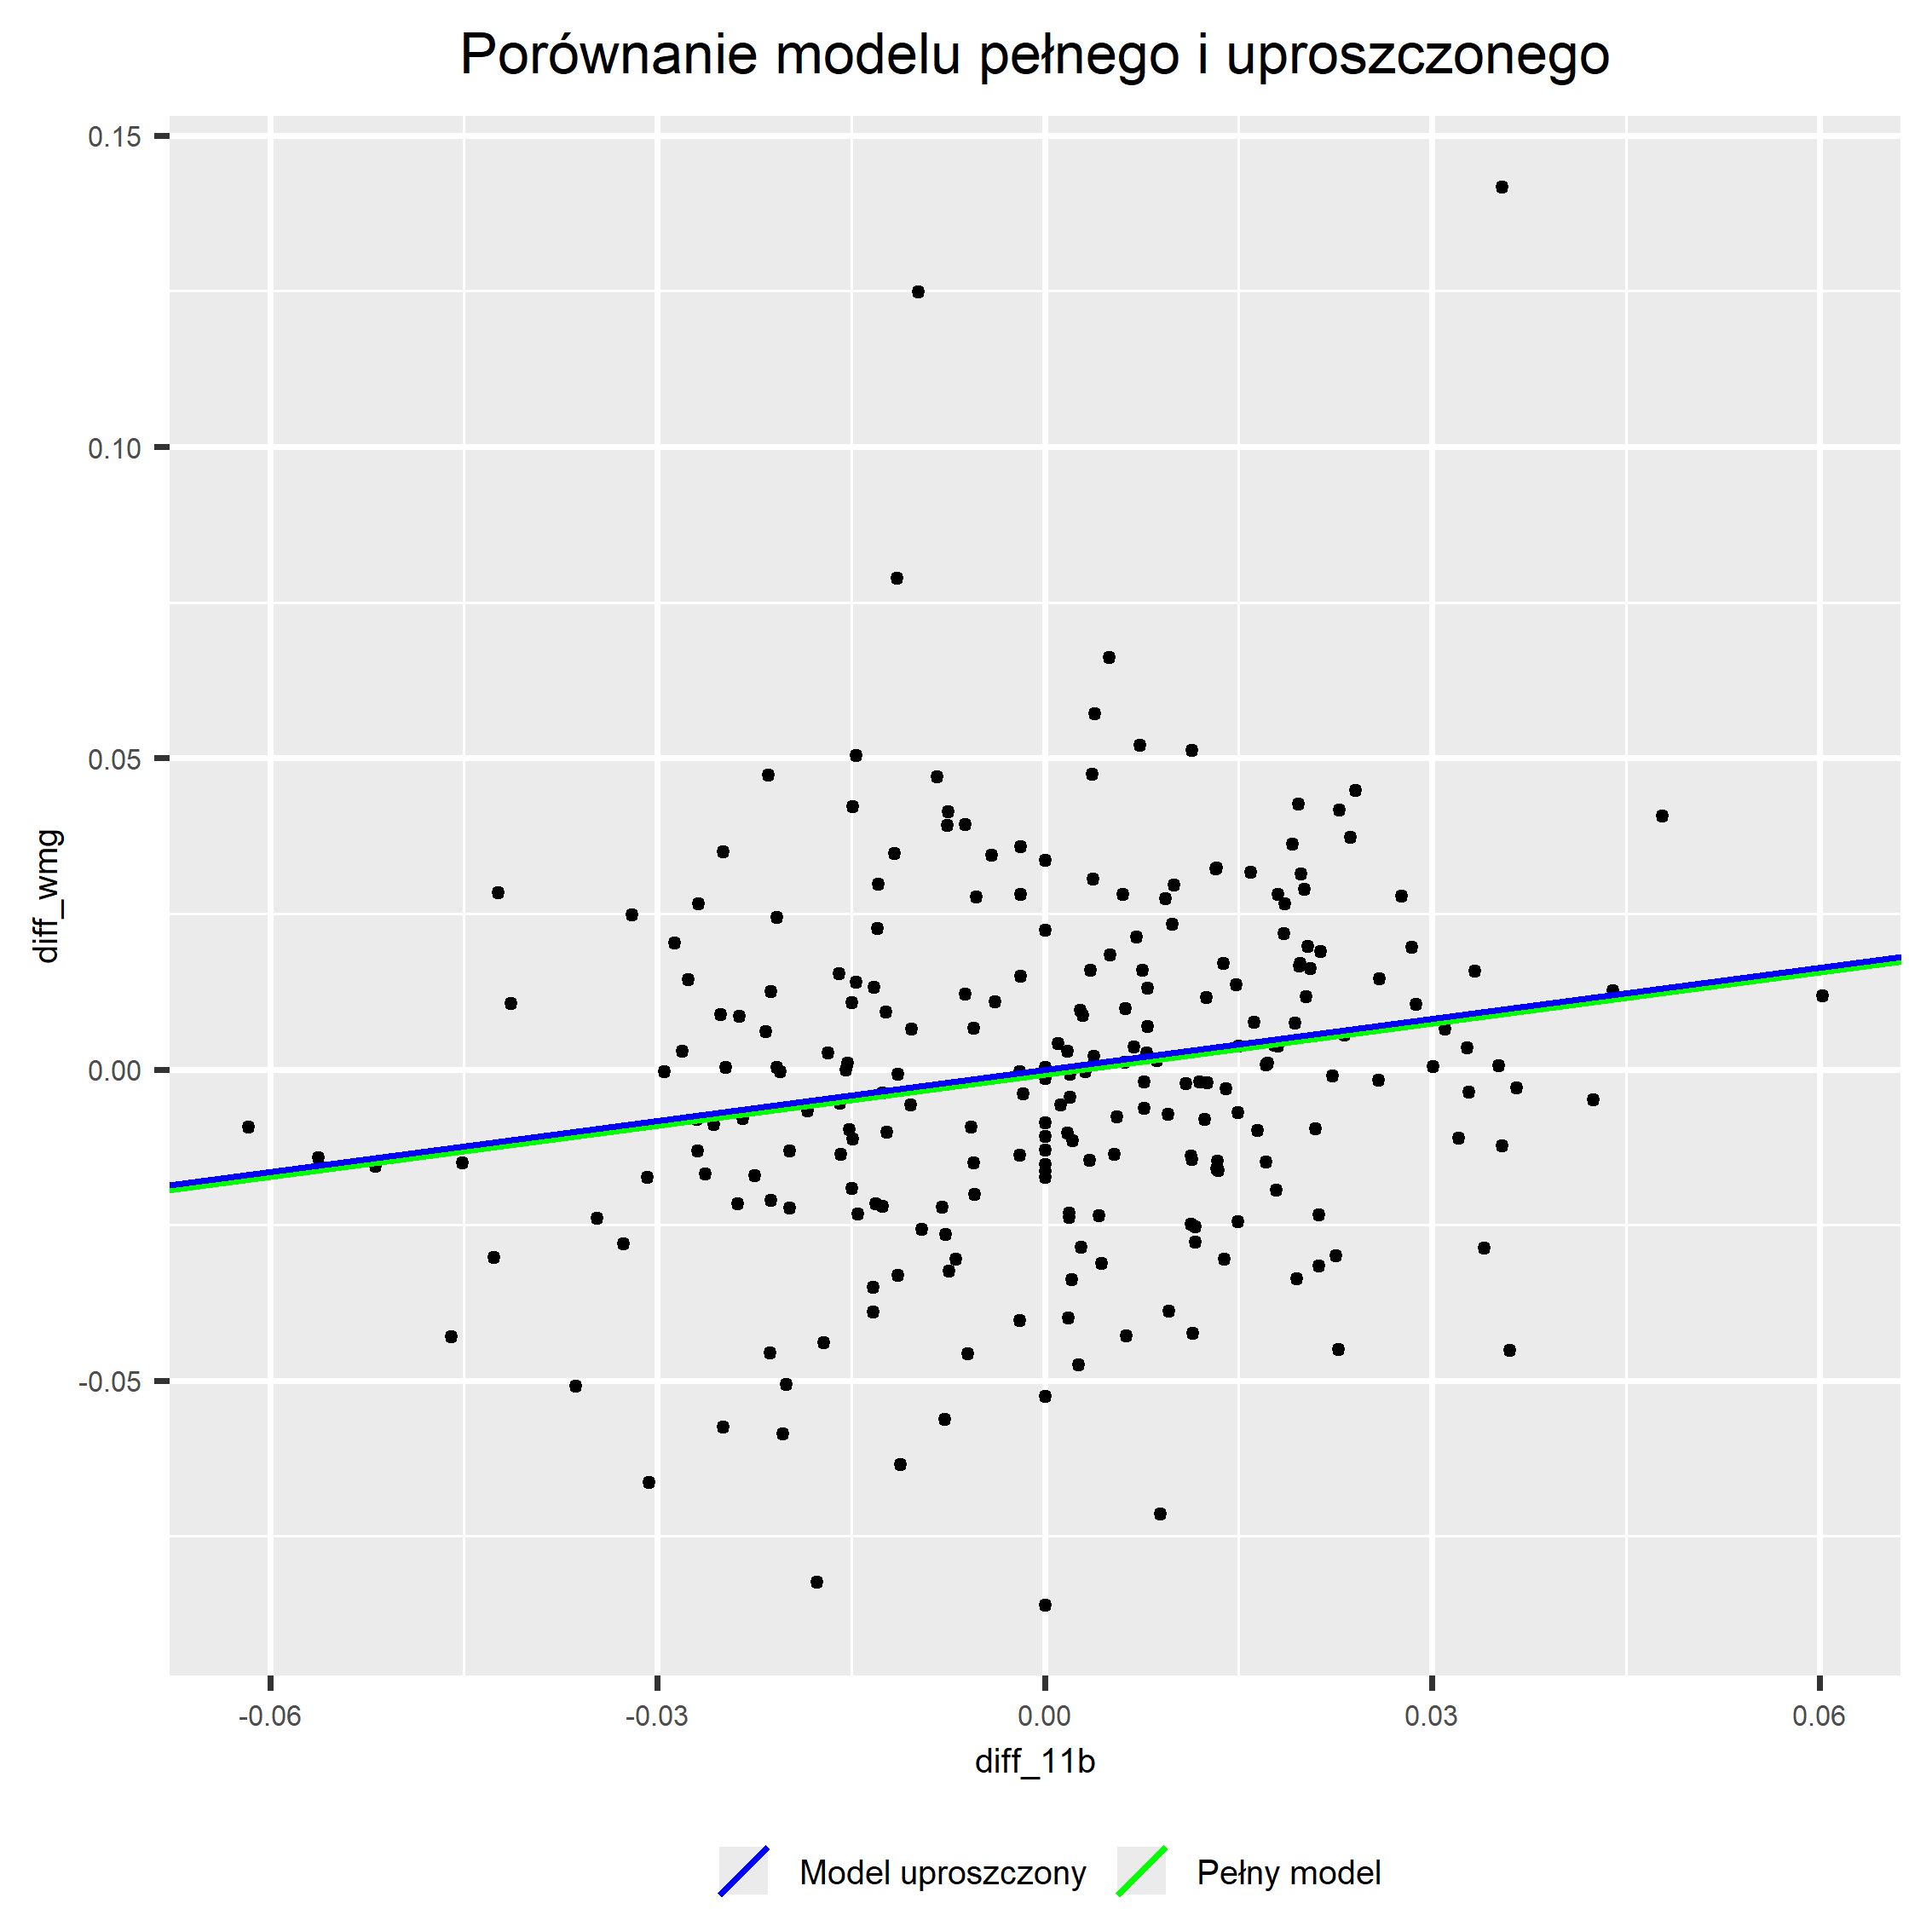
\includegraphics[width=12cm, height=12cm]{img/reg_porownanie_regresji.png}
\caption{Porównanie modelów regresji i uproszczonego}
\end{figure}

Zwracając uwagę na taki sam błąd standardowy reszt (RSE), współczynnik determinacji, a także nieznaczną różnicę współczynników \(b_1\) można stwierdzić, że \(b_0=-0.0008\) rzeczywiście okazuje się nieistotny dla stworzonego modelu regresji liniowej.

\subsection{Predykcja log-zwrotów dla modelu pełnego i uproszczonego}

Dokonujemy predykcji log-zwrotu spółki WMG.US gdy log-zwroty 11B będą na poziomie średniej ze wszystkich danych dla tej spółki. 

Za pomocą wzoru opisaną predykcję można zapisać następująco:
\[\hat{y}^* = \beta_0 + \beta_1 x^*\]

Dla opisywanych danych średnia ze wszystkich x-ów (log-zwrotów spółki 11B) wynosi:
\[x^* = 0.00026\]

a więc wzór na predykcję określa się:
\[\hat{y}^* = -0.0008 + 0.2738*0.00026 = -0.00076\]

\newpage
Wykres log-zwrotów spółek WMG.US i 11B z naniesionym pełnym modelem regresji liniowej i predykcją dla niego:


\begin{figure}[h]
\centering
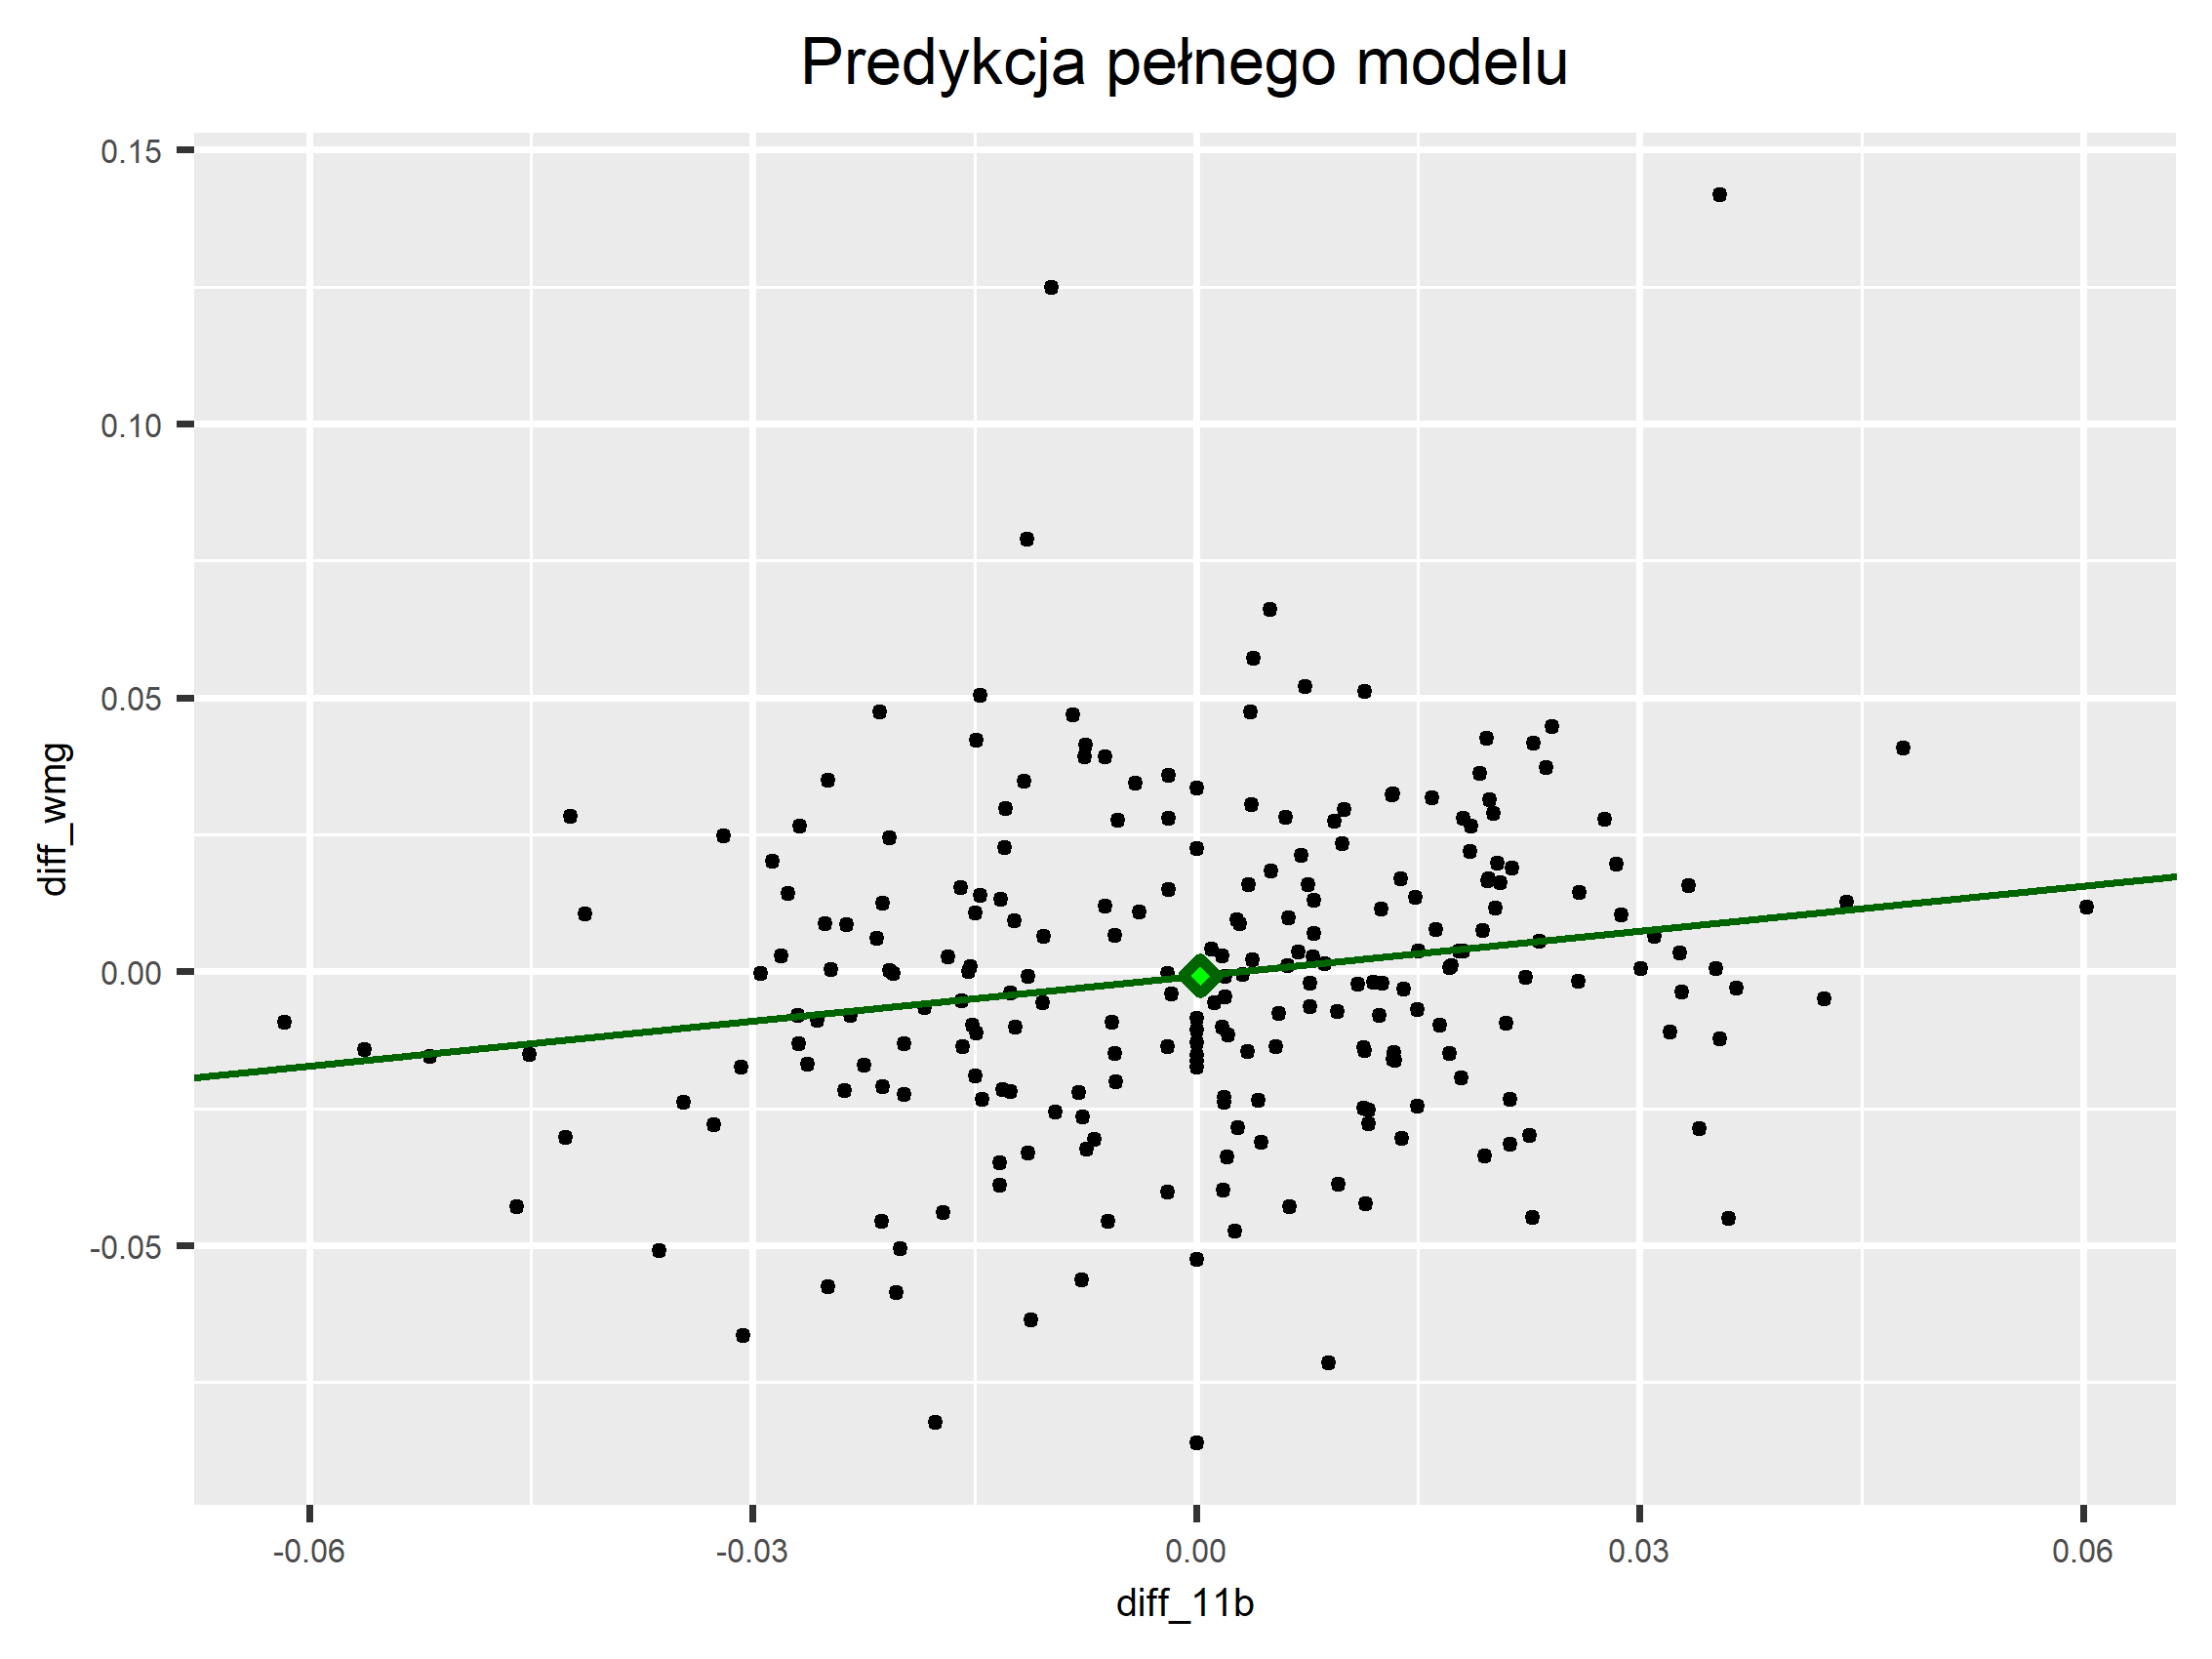
\includegraphics[width=12cm, height=9cm]{img/reg_pred_pelny.png}
\caption{Wykres log-zwrotów z naniesioną predykcją pełnego modelu}
\end{figure}

Predykcja na powyższym wykresie oznaczona jest jasnozielonym kolorem.
\vspace*{0.4cm}

\textbf{Predykcja dla uproszczonego modelu}

Średnia ze wszystkich x-ów (log-zwrotów spółki 11B) pozostaje bez zmian, a więc wynosi
\[x^* = 0.00026.\]


\(b_0\) w uproszczonym modelu wynosi 0, a \(b_1\) = 0.2733, a więc wzór na predykcję określa się:
\[\hat{y}^* = 0.2733*0.00026 = 0.0000709\]

\newpage
Poniżej znajduje się wykres log-zwrotów z naniesionym modelem pełnej regresji liniowej, uproszczonej regresji liniowej i predykcją dla obu modeli. Aby zwiększyć czytelność wykresu, a także pokazać różnicę w predykcjach, wykres został ograniczony do:

\[x \in [-0.02; 0.02] \quad \text{i} \quad y \in [-0.02; 0.02]
\]

\begin{figure}[h]
\centering
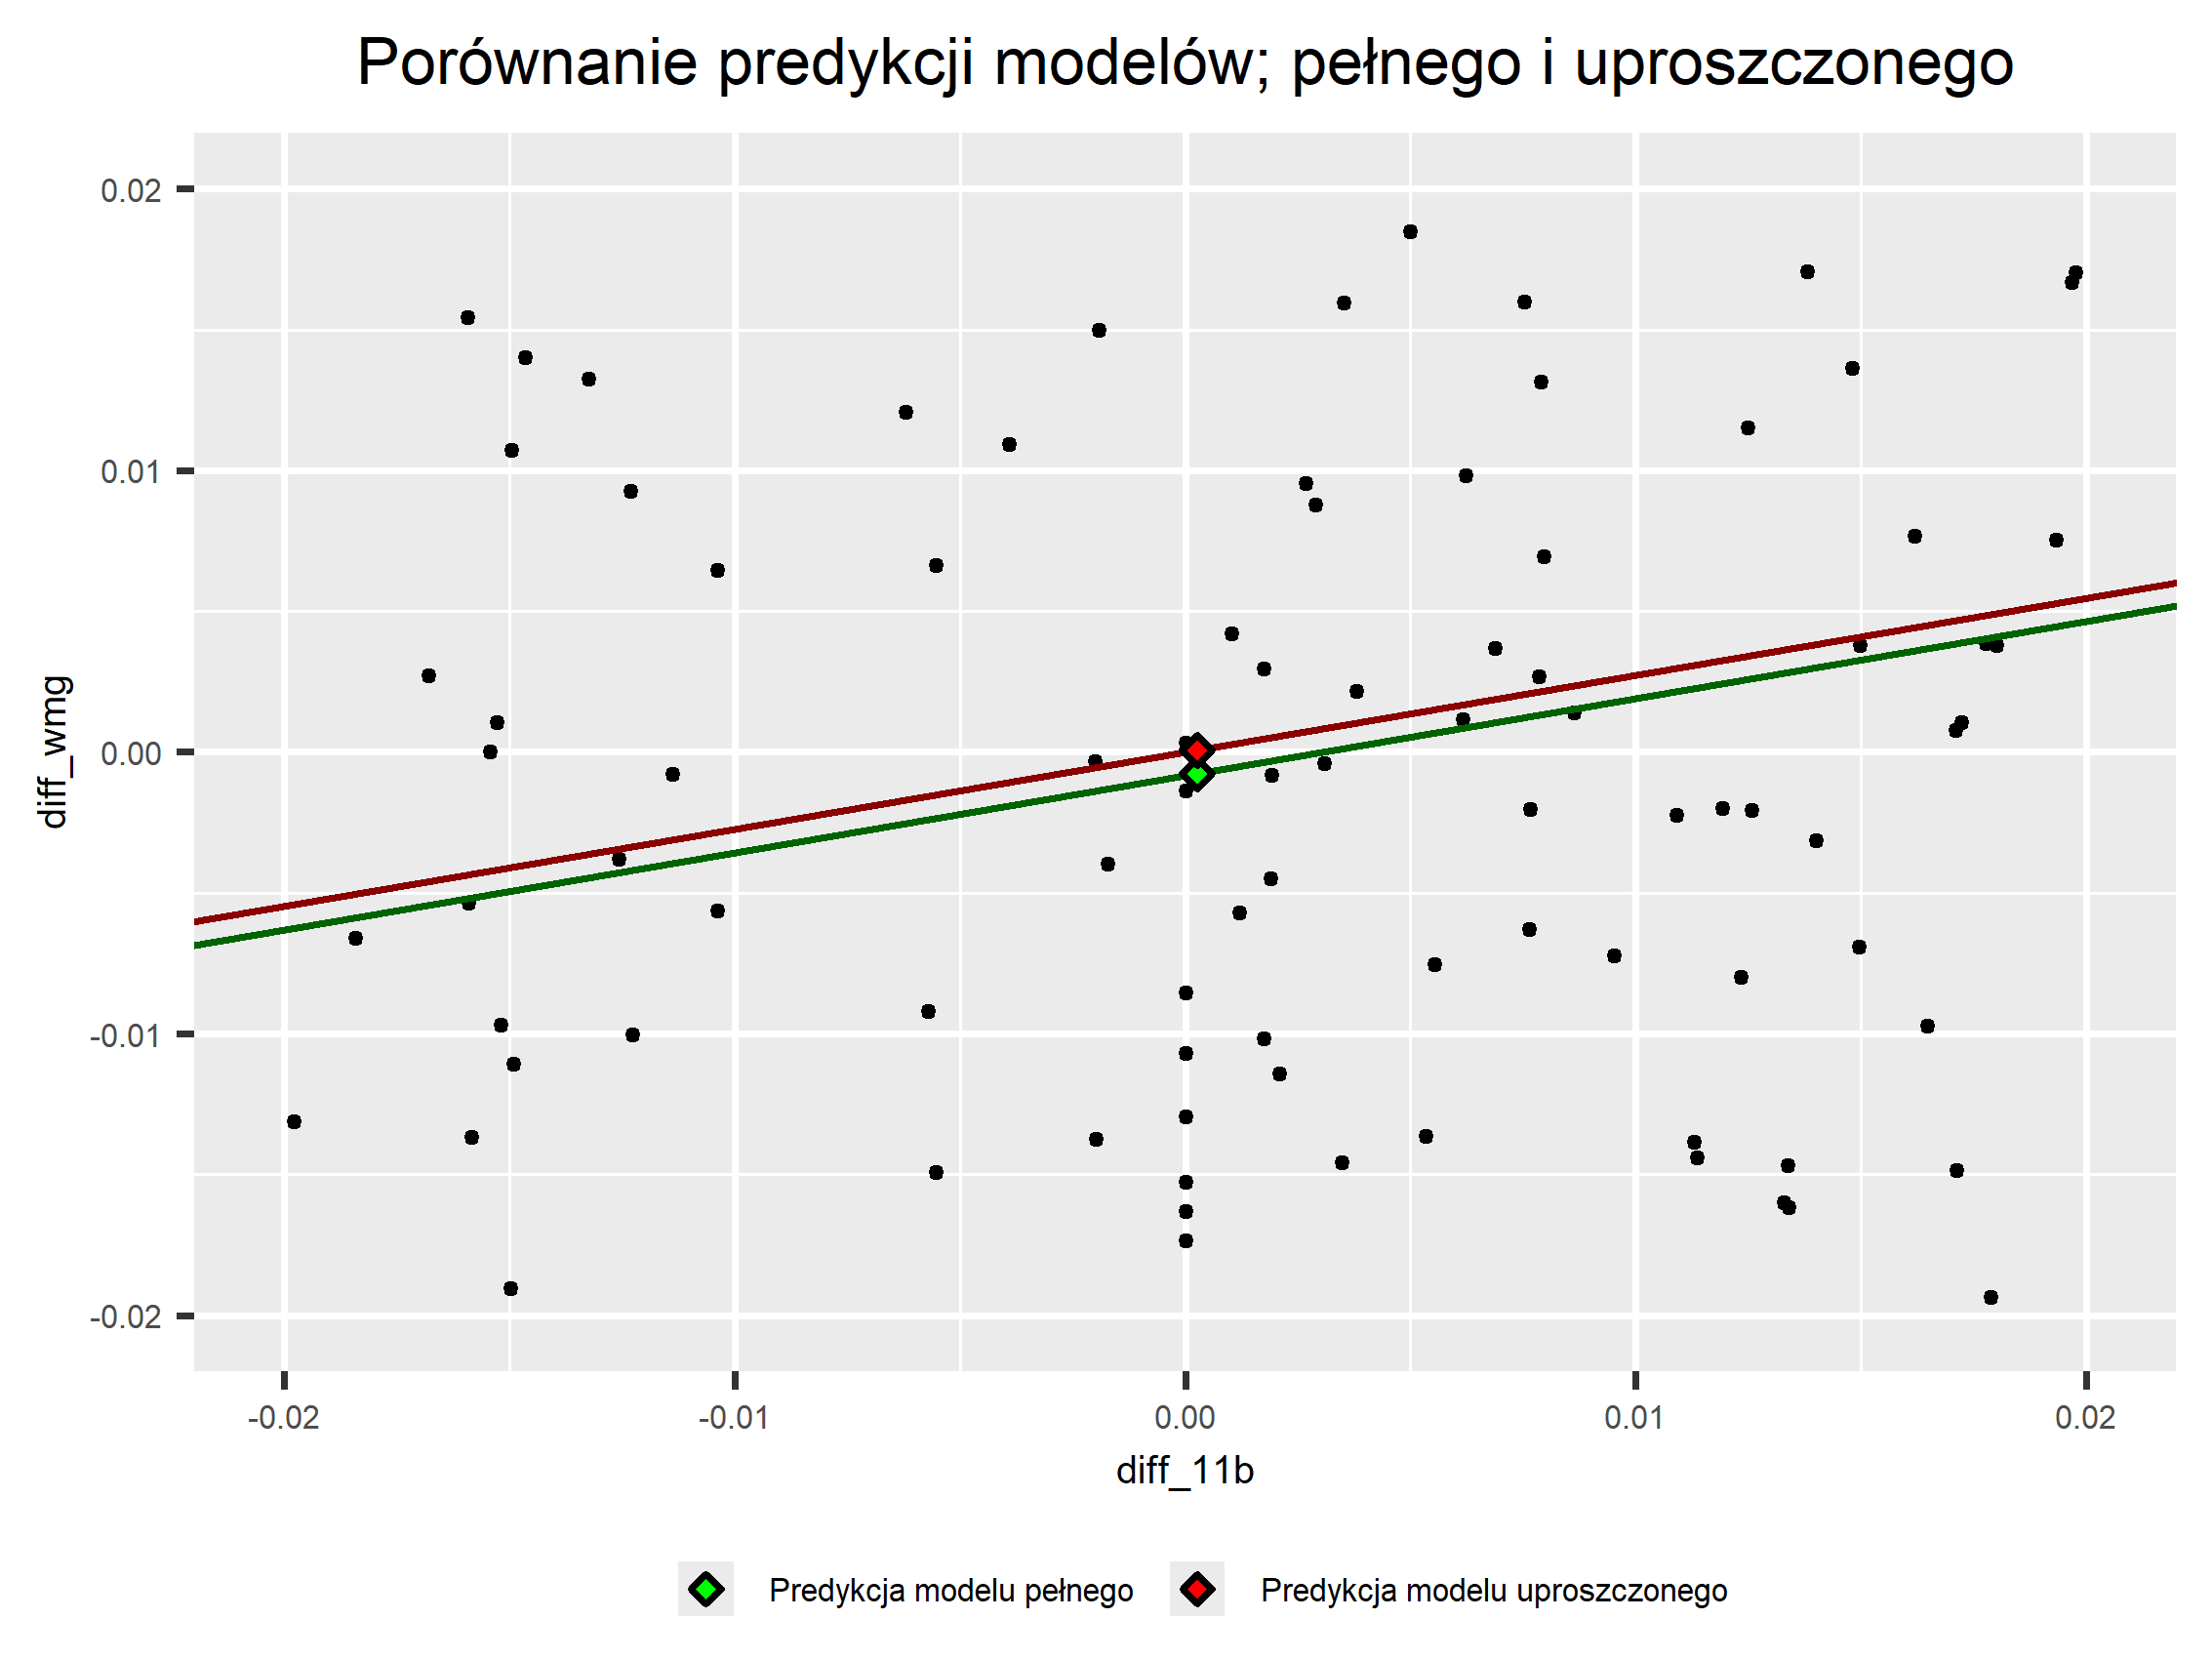
\includegraphics[width=12cm, height=9cm]{img/reg_pred_calosc.png}
\caption{Prównanie obu modelów, wykres powiększony}
\end{figure}

Z przedstawionego wykresu można zauważyć, że różnice w predykcjach są bardzo małe, jednak mimo tego różnią się znakiem: dla modelu pełnego predykcja jest ujemna, natomiast dla uproszczonego - dodatnia, choć wartości dla obu wynoszą praktycznie zero. Predykcja modelu uproszczonego ma więc wyższą wartość, choć jak już wspomniano, są to małe różnice.

\newpage
\section{Podsumowanie}
W przedstawionej pracy podjęto się badania i analizy cen spółek WMG.US i 11B 
Badania rozpoczęto od analizy każdej ze spółek osobno, gdzie przeprowadzono dopasowanie do rozkładu prawdopodobieństwa spośród trzech możliwości: rozkładu normalnego, log-normalnego i gamma. Dla obu spółek najlepiej pasował rozkład log-normalny. Następnie dokonano analizy wykresów diagnostycznych, statystyk opisowych, kryteriów informacyjnych i przeprowadzono test hipotezy o równości rozkładów metodą Monte-Carlo dla obu spółek, która w obu przypadkach nie została odrzucona.

Kolejnym etapem było przeprowadzenie analizy wspólnej dla log-zwrotów, obejmującej rozkłady brzegowe, dopasowanie każdego z nich do rozkładu normalnego, a także test hipotezy o równości rozkładów metodą MC, w której dla obu spółek nie odrzucono hipotezy zerowej: dane, czyli log-zwroty danej spółki można opisywać za pomocą rozkładu normalnego. Wyestymowano parametry rozkładu dwuwymiarowego normalnego:
\[
\hat{\mu} = \begin{pmatrix}
-0.0007550607 \\ % WMG.US
0.0002590858 % 11B
\end{pmatrix}
\]
\[
\hat{\Sigma} = \begin{pmatrix}
0.0008817645 & 0.0001082539 \\ % WMG.US
0.0001082539 & 0.0003953046 % 11B
\end{pmatrix}
\]

,a także wykonano analizę dobroci dopasowania. Dodatkowo przeprowadzono analizę dopasowania rozkładu \(\mathcal{N}(\hat{\mu}, \hat{\sum})\) do danych z której wynikło, że model, stworzony z parametrów rozkładu bardzo dobrze oddaje rzeczywiste dane.
 
Na zakończenie pracy zbudowano model regresji liniowej, analizując także reszty modelu \(\epsilon \sim \mathcal{N}(0, \sigma^2)\). Dla naszych danych wyglądał on następująco: 

\[y = 0.2738 * x - 0.0008 + \epsilon, \epsilon \sim \mathcal{N}(0, 0.029^2 )\]

. Sprawdzono istotność parametrów \(b_0\) i \(b_1\), a wyniki wskazały, że \(b_0\) jest nieistotny dla modelu. Stworzono zatem model uproszczony z \(b_0=0\):

\[y = 0.2733 * x + \epsilon, \epsilon \sim \mathcal{N}(0, 0.029^2 )\]

Ostatnim krokiem było stworzenie predykcji dla log-zwrotów WMG.US, przy założeniu, że log-zwroty 11B będą na poziomie średniej z posiadanej próby. Wyniosły one kolejno: dla modelu pełnego: (0.00026, -0.00076), a dla modelu uproszczonego: (0.00026, 0.0000709).

Cała praca dostarcza kompleksowej analizy modelowania matematycznego dla cen akcji obu spółek, uwzględniając różne aspekty statystyczne, estymację parametrów, testy hipotez oraz modelowanie regresji liniowej.

Wybrane spółki, a więc Warner Music Group i 11 Bit Studios wywodzą się z całkowicie różnych branż: WMG.US z branży muzycznej, natomiast 11B - gier komputerowych. Do tego pierwsza spółka większość swoich produktów kieruje w pierwszej kolejności na rynek amerykański, natomiast druga - na rynek światowy, z naciskiem na Europę. Z tego powodu można było wysnuć hipotezę, że analizowane ceny akcji tych spółek na rok 2022 nie będą miały ze sobą dużo wspólnego. Po przeprowadzeniu badań uważamy, że możemy potwierdzić tą hipotezę, a więc ceny akcji spółek WMG.US i 11B są od siebie niezależne i nie występuje żadna forma zależności lub korelacji.


\end{document}